%Import the Thesis formatting
\documentclass[12pt]{ucthesis}

%Package Imports
\usepackage[pdftex]{graphicx}
\usepackage{parskip}


\begin{document}
\title{Improvements and Analysis of Software Based 1200 Baud Audio Frequency Shift Keying Demodulation}
\author{Robert F. Campbell}
\degreemonth{June} \degreeyear{2014} \degree{Master of Science}
\defensemonth{June} \defenseyear{2014}
\numberofmembers{3} \chair{John Bellardo, Ph.D.} \othermemberA{Bridget Benson, Ph.D.} \othermemberB{Dennis Derickson, Ph.D.} \field{Computer Science} \campus{San Luis Obispo}
\copyrightyears{seven}
\maketitle

\begin{frontmatter}

\copyrightpage

\committeemembershippage

\begin{abstract}
Digital communications continues to be a relevant field of study as new technologies appear and old methodologies get revisited or renovated. The goal of this research is to look into the old digital communication scheme of Bell 202 and find a way to demodulate the signal in software with results similar to those of hardware demodulators. Even though there are software based approaches that are respectable in terms of being able to demodulate almost as many packets as hardware, the software demodulation is currently inferior. The research shows that through using Sivan Toledo’s JavaAX25 software package, new demodulation algorithms can be implemented that decode Bell 202 AX.25 encoded packets that the existing software tool could not.
\end{abstract}


\tableofcontents
\listoftables
\listoffigures

\end{frontmatter}

\chapter{Introduction}

Amateur Radio Operators, commonly referred to as "hams," make the best of resources available to them. However, once something is working a "don't touch it if it ain't broke" approach is often taken. Between these two mentalities some interesting phenomenon have occurred within the ham community. For example, some radio systems that are in active service today have only seen very minimal attention since the 1980's when they were originally installed. The implementation and development of the Automated Packet Reporting System (APRS) is no exception to the way hams approach things\,\cite{Bruninga}. Much of this system is based off older hardware and protocols - from the 1980s - that was readily available and few improvements have been made. Unfortunately, although the specification has been relatively stable there are inconsistencies. These inconsistencies include varying implementations from vendor to vendor as well as portions of the specification that are not clearly defined resulting in vastly inconsistent performance\,\cite{KWFThesis, KWFTAPR}.

So, what is APRS, and why does it matter? A brief introduction to APRS is that it is a digital communication scheme used by hams where a packet (whose content is varied, but is usually a GPS position - which is what gave APRS it's original name "Automated Position Reporting System"\cite{WikiAPRS}) is sent out over radio and then interpreted by other receiving stations. Figure \ref{APRSEndToEnd} shows one example of an end to end APRS system. A major challenge to this protocol and many other method of digital communication is the fact that it uses radio. Transmitting the signal wirelessly over radio means that it is susceptible to interference, weak signals as the distance from the transmitting station increases, as well as a myriad of other items. This research focuses specifically on the receiving end of these signals in order to see what improvements can be made to software based approaches to demodulating (decoding) these packets, which is represented by the TNC block in Figure \ref{APRSEndToEnd}. However, to more accurately portray software based demodulation the TNC block in the figure should be moved inside of the computer block since the receive radio audio is passed straight to the computer and then interpreted by this special software.

\begin{figure}
  \centering
	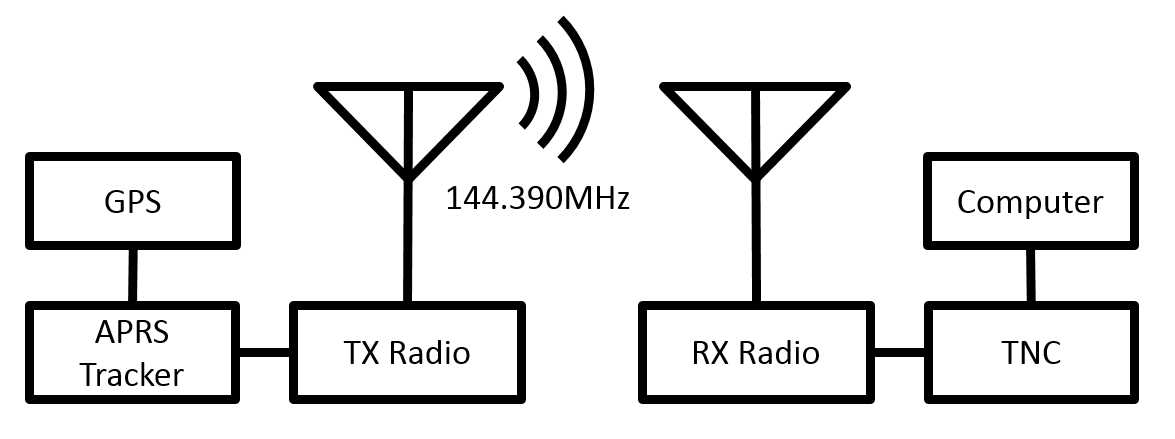
\includegraphics[width=0.75\linewidth]{images/APRSEndToEnd.PNG} 
   \caption[Block diagram of an example APRS system end to end.]{Block diagram of an example APRS system end to end. The GPS communicates information using NEMA to the APRS tracker, the tracker then takes this information and the preferences in its configuration to formulate APRS packets. The APRS packets are encoded by the tracker and the resulting audio passed to a transmit radio which sends the data. Typically this is done on frequency 144.390MHz in the United States. Receiving radios tuned to the same frequency pass the received audio to a TNC which decodes the packet and passes it to a computer using RS-232.}
   \label{APRSEndToEnd}
\end{figure}

The reasoning for trying to make improvements in software based demodulation are many, but a few of the more motivational ones are to follow. One advantage of doing software based demodulation is that it removes the necessity of specialty hardware; Instead of having dedicated hardware whose sole purpose is to modulate and demodulate APRS packets, hams can use a computer to do these tasks. By using a computer's sound card, audio from the radio can be processed using software to decode received packets, or audio can be played from the sound card to the radio to be transmitted. With the abundance of personal computers, this can provide a much cheaper solution for hams who are interested in trying out APRS without having to put down a potentially big initial investment (\textasciitilde\$200\,\cite{Kantronics2014,Outlet2014}) for a piece of hardware that serves one purpose. The price of this specialty hardware is steep and it is limited to only performing communication on a single channel. When using a line in / out on a computer they are typically stereo, meaning that a single sound card could handle operations on multiple channels. If two channels just is not enough the capabilities of a computer demodulator can be expanded by merely adding another sound card which is relatively cheap at \textasciitilde\$20\,\cite{Newegg}. See Table \ref{costCompareTable} for a comparison of the cost for hardware and software. From the table it can be seen that the cost to perform communication on 4 channels using dedicated hardware the cost would be \$800! For this cost a whole computer with a half dozen sound cards could be purchased, only further expanding capabilities.

\begin{table}
	\begin{center}
		\begin{tabular}{ | l | r | r | r | r | }
		\hline
			Cost for: & 1 Channel & 2 Channels & 3 Channels & 4 Channels \\ \hline
			Software & \$0 & \$0 & \$20 & \$20 \\ \hline
			Hardware & \$200 & \$400 & \$600 & \$800 \\
			\hline
		\end{tabular}
		\caption[Hardware and Software Cost Comparison]{Cost comparison of conducting APRS communications on 1 through 4 channels for hardware versus software assuming the user already owns a computer.}
		\label{costCompareTable}
	\end{center}
\end{table}

In addition to the the price advantages of software based demodulation approaches, there is also one other primary advantage. If software is being used instead of hardware there is the potential for a lot more capabilities since processing power and available memory increase drastically. For instance, one of the dedicated hardware solutions, the Kantronics KPC-3 Plus, has a mere 512KB of memory compared to that of any computer which is over 4GB as of 2014 - and that is just the ram, not hard drive space\,\cite{Kantronics2014,Graham-Smith2014}. Additionally, instead of just being able to handle live events and process each data point in the best manner possible as soon as it comes in, post processing becomes an option.

With the cost and versatility of a software demodulation solution now introduced, the paper addresses the following: Chapter 2 goes into background information, with a deeper introduction to APRS and a presentation of the aspects important to understanding this research. In Chapter 3, some of the current methods for interfacing with APRS, both hardware and software, are explained. Demodulation techniques are discussed in Chapter 4. Chapter 5 talks about the challenges of demodulating APRS packets. Chapter 6 discusses the methods used for benchmarking and comparing the demodulators. In Chapter 7, information on how the demodulators and algorithms are tested is presented. Chapter 8 goes into more detail about the software implementations in this project. Chapter 9 discusses the results of both the newly implemented algorithms and compares them to other demodulators. Areas of additional research and future work are discussed in Chapter 10. Chapter 11 is concluding remarks.

\chapter{APRS Background and Definitions}
From the introduction it is known that APRS is a method of digital communication used by hams in order to inform other hams of their location. In addition to supporting sending positions, APRS can be used to send messages, bulletins, weather, and other information. Since these packets are transmitted via radio  - which has limited coverage - APRS can be viewed as a local area awareness network. This gives hams who are listening for and decoding APRS packets information about nearby transmitting stations. This brief overview should give a little insight into APRS, but the rest of the section will focus more on what is going on behind-the-scenes to explain how APRS works in terms of the protocols, data transmission, modulation, etc.

In order to organize this discussion of the different components of APRS let us break it down into the Open Systems Interconnection (OSI) model representation. However, before fitting it into the OSI model here is a brief reminder of the relevant layers that are going to be discussed. Layer 1 of the OSI model is the physical layer. The physical layer consists of everything that is used to transport one bit of information from one location to another. The second layer is the data link layer. Within the data link layer bits from the physical layer are passed up to the network layer, and information from the network layers is framed and handed off to the physical layer. Layer 3 is the Networking layers. This Layer is responsible for determining the path that packets will take and providing flow control to prevent flooding. Above these layers are layers 4-7 which are the transport, session, presentation, and application layers respectively \cite{Sosinsky2009}. These upper layers get too inter-tangled to be able to cleanly separate them. For instance within the AX.25 2.2 specification a TNC is mentioned that only implements layers 1, 2, and 7 of the OSI model \cite{Beech1998}.

Here is the best division of APRS into the OSI model, following introducing this division each layer will be individually discussed in more detail. Layer 3 of the OSI model for APRS is the the AX.25 Protocol,  High-Level Data Link Control (HDLC) protocol composes layer 2. All the way at the bottom, layer 1 for APRS consists of the Terminal Node Controller (TNC) and Radio \cite{Silver2013}. A brief note on why the discussion begins with Layer 3 is because this is how the data is transferred. The interest stop here and does not continue to the layers above layer three, because those are all application specific. Starting with AX.25 the background information will be given down to Layer 1 which is where this research actually aims to make a contribution.

\section{Layer 3 - AX.25}
Layer 3, the network layer, is responsible for routing frames between individual nodes in the network. A frame of data is more traditionally called a packet at this point since AX.25 is a packet switched network protocol \cite{Peterson2011}. AX.25 is the amateur X.25 protocol. Meaning that the AX.25 protocol, which is what APRS uses, was developed my Amateur radio operators and is based off of the x.25 protocol. Since the origins of AX.25 lie within X.25, the discussion will begin with X.25. 

\subsection{X.25}
Developed in the 1970s the packet switching protocol X.25 was deployed on telephone networks where it was used until it began to be displaced by the IP protocol. The X.25 protocol suite provides OSI layers 1-3, although it does have standards that support each of those layers \cite{Sosinsky2009}. For instance the X.21 standard is commonly used for layer 1 of X.25 and ISO 7776 specifies a Link Access Procedure Balanced (LAPB) to assists with layer 2, the data link layer \cite{Gallagher1997}. The Data Link layer of LAPB, a bit oriented protocol derived of HDLC,  manages packet framing and ensures that frames are error free and properly sequenced. When used on telephone networks there were five distinct modes that the protocol would operate in: Call setup for establishing the connection, Data transfer, idle where the connection is established but no data is being transferred, call clearing for terminating the connection, and restart for resynchronizing the host and client \cite{Javvin2006}. Many of the features of the Layer 2 and Layer 3 operations of X.25 can be found in at least a similar fashion in AX.25.

\subsection{AX.25}
Next the AX.25 protocol will be discussed through comparison and contrast with X.25. One of the main differences between the X.25 and AX.25 is that when the specification is read, in addition to specifying the behavior of Layer 3, the behavior of Layer 2 is also included. Although this is somewhat implied for X.25, there are still separate documents for the specifications for each one of the layers. After reading the specification for AX.25 it very clearly defines the framing with starting and terminating flags as well as the networking and routing \cite{Beech1998}.

\section{Layer 2 - High-Level Data Link Control}
The goal of HDLC is to make sure that when the data is received and passed up to Layer 3, that it is error free, without loss, and in the correct order \cite{Javvin2006}. There are a few ways that HDLC accomplishes this, two of which are framing and with the Frame Check Sequence (FCS). The framing occurs through the use of flags around the data. A flag is one byte and is hex 0x7E. For APRS common practice is to send multiple flags consecutively to give transmitting radio time to key up and settle or to give receiving radios time for their squelch to open. Since it is an non-return to zero inverted (NRZI) encoding no change in frequency corresponds to a 1 and a change in frequency corresponds to a 0. As such multiple 1s in a row make it hard to keep timing which is why bit stuffing is used. With the exception of the flag which contains six consecutive 1s (01111110) if there six or more consecutive 1s in the data packet a zero will be stuffed after the fifth 1 to increase the clocking energy in the signal.

\section{Layer 1 - The Bell 202 Modulation and the Radio}
Since Layer one is composed of the things needed in order to transmit one bit from one location to another, it needs to be made clear what all this includes for APRS. Starting with air, the medium through which the radio frequency (RF) signals propagate, the RF transmissions are received or transmitted by the radio. Without decomposing the radio into all of its individual components, the audio that the radio receives then has to be processed. In order to stay focused on what happens in layer 1 and not start mixing the other layers together some more discussion of what this audio signal consists of is necessary.

The audio signal that contains the APRS packets is composed using the Bell 202 modulation which is an Audio Frequency Shift Keying (AFSK) mode. As such RF either comes in through the radio, is translated to the corresponding audio, and then demodulated into a bit stream by interpreting the Bell 202 modulation. Or, a bit stream from layer 2 of APRS is modulated using the Bell 202 modulation, this modulated audio is passed to the radio, and the radio then transmits it out. Since decomposing the radio down into its individual components does not have any affect on representing the different OSI layers of APRS, it will not be discussed. However there are factors that affect wireless communications and RF signals that will be discussed in chapter 4.

\subsection{Frequency Shift Keying}
In order to understand the Bell 202 modulation scheme the communication mode of AFSK needs to be introduced. AFSK is a form of frequency shift keying (FSK) that occurs by modulating frequencies in the audible range. FSK uses multiple frequencies in order to represent the different symbols such as 1 or 0 or mark and space in our case. If the frequency of the data carrying signal can be determined, then the symbol is knows for that bit period. FSK is the more generic term and is used for 9600 baud (bits per second) APRS on Ultra High Frequencies (UHF). In this mode the actual RF carrier in the 440MHz band is modulated between one frequency and another nearby frequency in order to represent the two different symbols. In contrast, AFSK switches between two different audio signals, which for APRS on Very High Frequencies (VHF) is then modulated onto the RF carrier using Frequency Modulation (FM).


\subsection{Bell 202}
With FSK and AFSK now introduced the AFSK used within Bell 202 can be described. The Bell 202 modem was patented in 1984 using 1200Hz and 2200Hz tones, although the patent was originally filed in 1981 \cite{stauffer1984fsk}. Interestingly, the International Telecommunication Union (ITU) did not publish a standard for this modulation that were used in telephone networks until 1988. In the standard, however they use 1300Hz tone for symbol 1 and 2100Hz tone for symbol 2 called a mark and space respectively \cite{ITUV23}. The original bit stream is modulated using a non-return to zero inverted (NRZI) encoding. This means that when a transition occurs from one symbol to another in the Bell 202 modulated signal this symbolizes a 0 bit in the original data bit stream and if the Bell 202 symbol remains constant over multiple symbol periods, that signifies a 1 bit in the original data bit stream. For Bell 202 the frequencies that are used are 1200Hz and 2200Hz tones for the mark and the space as opposed to the 1300Hz and 2100Hz tones proposed in the ITU specification.

\chapter{Current APRS Demodulation Approaches}
In the world of APRS there are many solutions that hams use to be able to utilize the network. Some they find and make work, some they purchase to use exclusive for APRS, and some go through the trouble of inventing their own solutions. This chapter explains some of the common systems used on the APRS network, primarily those that can be used for receiving, starting with terminal node controllers and progressing to software based demodulation.

\section{Terminal Node Controllers}
Currently there are many systems that will demodulate these Bell 202 encoded APRS packets. The original hardware used for this communication style was dedicated modems similar to dial-up 56k modems that did the encoding and decoding. These modems were connected directly to the radio and the radio would let the modem know through a signal pin if the radio was receiving what it thought was a data carrying signal. The terminal node controller (TNC), a modem used in AX.25 operation, would let the radio know by signalling the radio to transmit when it had data to send out.

%%%Potentiall needs some editing - TO DO%%%
%As mentioned in the introduction and early in this section, the technologies that are being used for this data transport originated in the late 1980s even though the spec for the protocol itself did not get officially released until 2000. This serves as a reminder that old hardware is commonly used that is not well understood. If a user gets something reasonable working, they will use it without doing a full analysis on edge cases or making simple modification to improve performance.

With a radio and a Terminal Node Controller, amateur packet stations and digipeaters (digital packet repeaters) are possible. Digipeaters are an essential part of the ham packet network, but many users wish to report their GPS position onto the APRS network instead of just relaying traffic for other stations. In order to accomplish this, a GPS receiver is required. Now, stations can take the data from their GPS receiver and put it in the payload of the APRS packet and transmit the GPS reported position onto the network. Within the testing scope of this project there are two TNCs whose decoding results are compared to the software approaches. These two modems are the AEA PK-88 and the Kantronics KAM Plus. However, the PK-88 and the KAM Plus although used very frequently in APRS systems are not fully dedicated hardware for APRS, but instead modems that are being used for ARPS.

\section{Specialized APRS Hardware}
Many people know exactly what they would like to do with APRS and exactly what traffic they want to contribute to the APRS network. This has allowed for companies to start commercially making dedicated APRS hardware, since there is a demand for it. In addition to making this hardware available the produces support the hardware and make pretty user interfaces for the users to be able to program the hardware exactly as they like and without having to invest much time into understanding how different components work together. Some examples of APRS exclusive devices are ArgentData�s OpenTrackers, Byonics� TinyTrack, and Fox Delta�s Fox Track \cite{Miller,Byonics,Foxtrak}. These compact packages along with a radio and a GPS module perform APRS tasks at a satisfactory level for many users.

Since the average user only wants to report positional information, these dedicated devices are simple to setup to do such but also only include a simple feature set. Although these trackers contain some features, since they are basically small embedded systems they do not have all of the features that APRS support. An example is the messaging service. Since these devices don�t have a display or a keypad, there is no way to input or display a message. Certain radio manufacturers have begun to integrating the TNCs into the radios themselves to utilize the radio�s screen. The Kenwood TM-D700 series and Yaesu FTM-350 are examples \cite{Kenwood,Yaesu}.

However, both the options that were presented in this section and the one previous on TNCs require going out and buying special hardware in order to perform APRS whether it be a TNC itself of a OpenTracker. This can be expensive and cost prohibitive for some hams to be able to begin APRS operations.

\section{Software Based Demodulation}
%Copied from old Software Based Demodulation
It can be assumed that before a ham operator becomes interested in the APRS network and sending APRS packets that they will already have a radio. So, if they already have a radio all they have to do is buy a piece of hardware that will do the modulation in order to send a packet. However, hardware costs money and before diving right in it might be nice to get their feet wet first. A good, cheap alternative to dedicated hardware is to use hardware that hams already have. A good choice that will fit the needs is a computer, which most hams probably own at least one of. On this computer amateurs can build or buy a cheap interface to a radio, ~$15 instead of ~$150 for a piece of dedicated hardware, and then use software to do the modulation and demodulation.

This seems to be a route that some are taking and a demodulation scheme that this project explores in detail, but first some more information on current systems that operate in this software realm. Some examples of the software that can be used are George Rossopoylos�s Packet Engine \cite{Rossopoylos} or Thomas Sailer�s Linux Sound Modem \cite{Sailer1997}. On a computer, even ones with minimal resources, there are algorithms that are being used to demodulate the APRS packets. Again, what this project aims to investigate is what improvements can be made to the algorithms and software based demodulation approaches in order to decode these packets in a more robust fashion and to try and get similar performance to TNCs and dedicated hardware. 

Preliminary testing shows that the software still has room for improvement in order to be at least as good as TNCs. As mentioned thus far, software provides a viable low cost alternative to dedicated hardware, but is just that - a cheap solution. It still has some weaknesses that need to be addressed, and refinements to be made to improve demodulation to match performance of hardware. 

%!!!!!!!!!!!!NEED MOTIVATION... EXPLAING PROS OF SOFTWARE HERE...!!!!!!!!!!!!!
\chapter{Demodulation Challenges}
While analyzing different demodulation algorithms and trying to improve their performance, there were a few phenomena that were observed. Specifically, there were aspects that proved problematic for software based demodulation, and although they are probably challenges to all types of demodulation and not just those that are software based, they were noticed during these analyses. While inspecting performance of the algorithms the following items created difficulty and can all be attributed to the fact that APRS uses RF and hence is susceptible to all the items relating to an RF transmission. 

The main challenge in decoding the APRS data was the fact that the digital stream is converted to an audio signal and then transmitted over RF. The addition of RF adds a whole plethora of obstacles which can include Path Loss, Multi-path, Fading, Doppler effects, Co-channel interference, Interference and Noise, and Foliage \cite{Goleniewski2006}. A few items which are important to note, due to the fact that some of the algorithms had to be coded to tolerate them are: DC Offset, Noise, and Emphasis.

\section{Challenge: DC Offset}
An audio signal can be characterized by a sine wave. In order to get different sounds the frequency of the sine wave is changed and in the context here, the two frequencies are 1200Hz and 2200Hz. Since an audio signal is a sine wave, the average value should be zero. The zero value is commonly referred to as the ground of the audio signal, and as the definition would imply the signal should spend the same amount of time above ground as it does below ground. As the performance of zero crossing algorithms were investigated it was very evident that this was a challenge. If one assumes that the signal is centered about zero, and it is not, the logical decisions made with this incorrect assumption will hence not hold true. Figure \ref{DCOffsetExample} shows that the signal is not centered around zero. This lack of the signal being centered around 0 (or ground) is why it is said to have a DC offset. It can be noticed in this figure that near the center there are time periods that would be both much longer and much shorter than those expected from subsequent zero crossings during demodulation due to this DC offset effect.
\begin{figure}
  \centering
	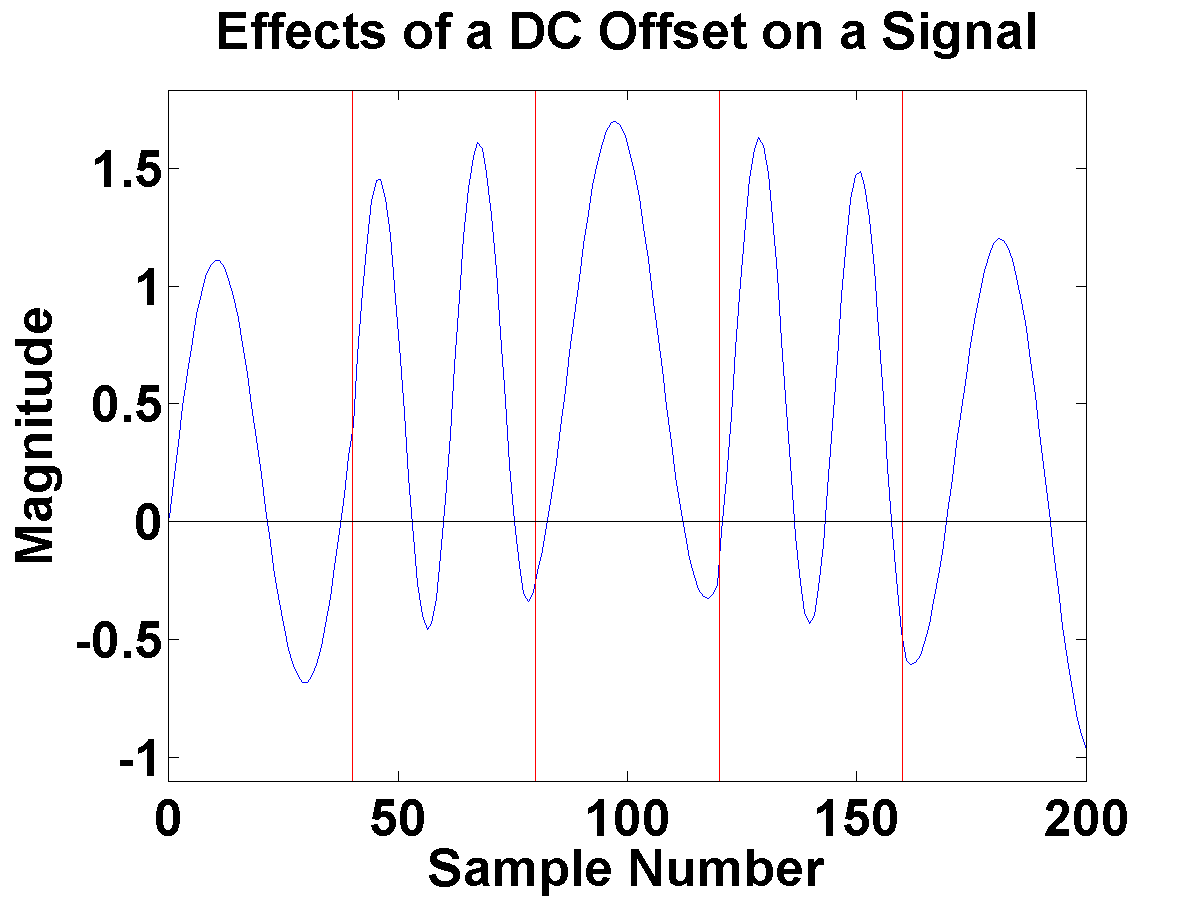
\includegraphics[width=0.75\linewidth]{images/EffectsofaDCOffsetonaSignal.png} 
	\caption{An example Bell 202 signal with a DC offset problems.}
   \label{DCOffsetExample}
\end{figure}

\section{Challenge: Noise}
First, a definition of noise in this context: noise refers to unwanted electrical signals present in electrical systems \cite{Sklar1988}. Since the data is an AFSK signal that is then frequency modulated, there are two distinct steps where noise can be introduced, but must be kept to a minimum to increase the chances of the data properly decoding. Hence, the a large signal to noise ratio is preferred. This is not the case for only APRS but with all wireless technologies. One cause of noise is increased distance between the transmitter and receiver. An example that many are probably familiar with is as a client gets farther away from a wireless access point the bandwidth decreases. This happens because the signal strength drops off at 1 / distance cubed \cite{4Gon}. What was noticed when some of the algorithms were being debugged was that the random noise that could be inflicted due to the nature of transmitting a wireless signal caused significant problems.

One such example of this is if the noise happened to also take on the form of a sine wave and the algorithm locked onto that frequency instead of the 1200Hz or 2200Hz signal that was wanted to be decoded. Alternatively, if the noise was just random and jostled the signal in the correct spot 1200Hz tones might look like 2200Hz (this ended up being fairly common) or vice versa. An example of what noise may look like on the original signal is in the Figure \ref{noiseExample}.
\begin{figure}
  \centering
	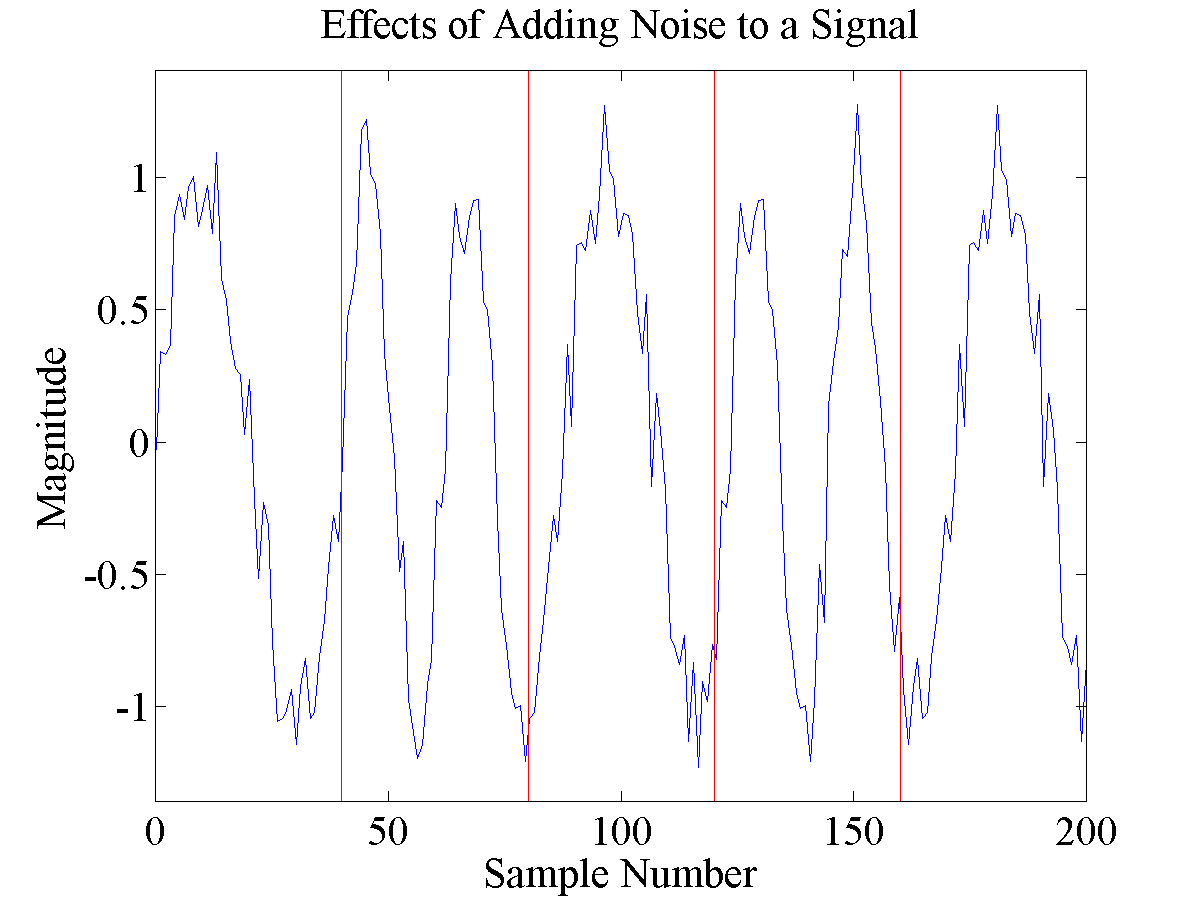
\includegraphics[width=0.75\linewidth]{images/EffectsofAddingNoisetoaSignal.png} 
	\caption{An example Bell 202 signal with white noise added.}
   \label{noiseExample}
\end{figure}

\section{Challenge: Emphasis}
Due to the fact that this is AFSK data being transmitted over a voice channel, emphasis becomes a concern. Preemphasis is when the the higher audio tones in a Frequency Modulated (FM) signal are intentionally increased and deemphasis is when that process is reversed on the receiving end to return the audio to a flat signal. Why emphasize the audio signal? This process of emphasis is not necessary, but the effects are desirable since it increases the signal to noise ratio in the RF signal by having the higher audio tones preemphasized \cite{Gibilisco1994}. The reason this is a concern is because the adoption of emphasizing and deemphasizing APRS signals is inconsistent. Some radios have data ports which bypass the emphasis step while other APRS users utilize the Mic and speaker ports of a radio which would utilize emphasis. This would mean that a signal transmitted out of a radio with a data port may not be emphasized, but then when received through the speaker out of another radio would be deemphasized. The effects of a non-emphasized signal being deemphasized can be seen in Figure \ref{emphasisExample}. This causes problems with the demodulation because it can not be assumed that the relative powers of each frequency will be equal since they will have different magnitudes in this case. 
\begin{figure}
  \centering
	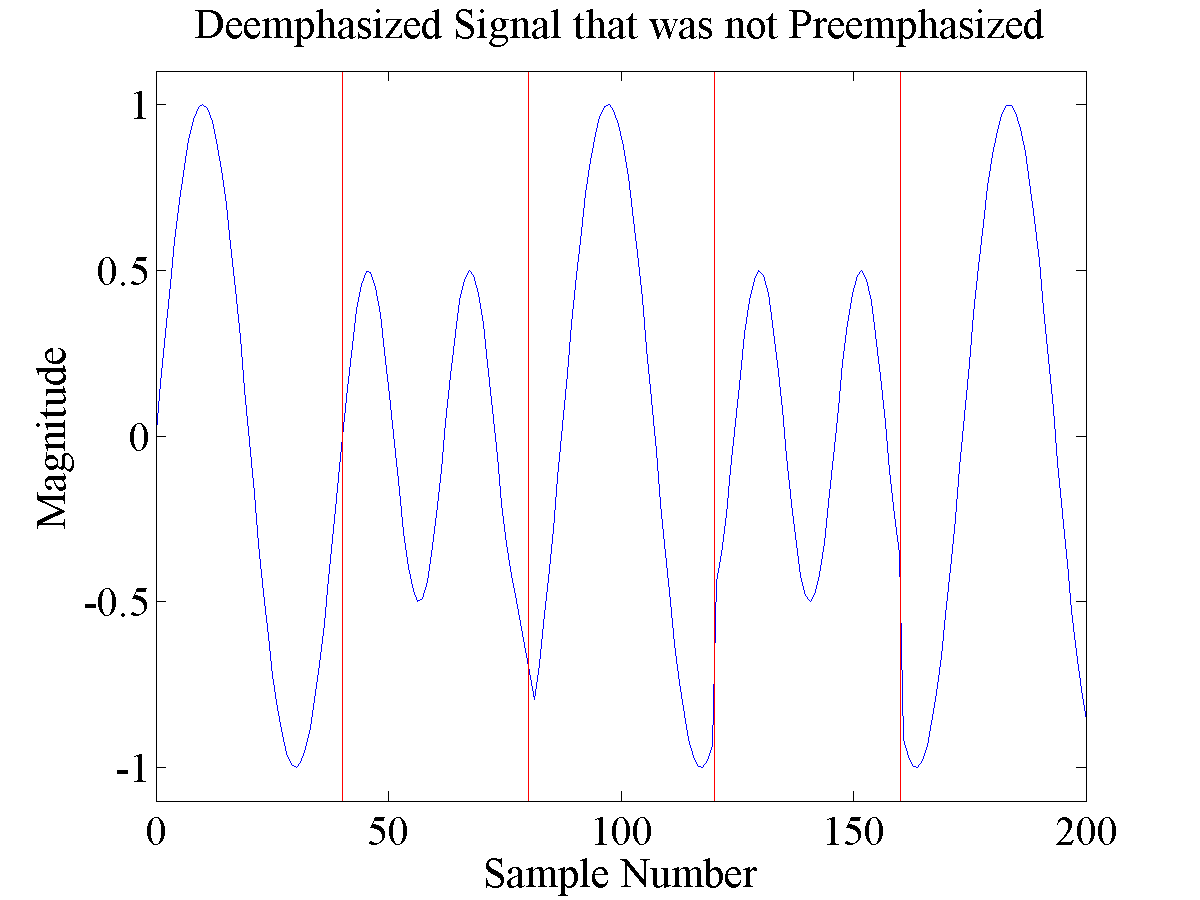
\includegraphics[width=0.75\linewidth]{images/DeemphasizedSignalthatwasnotPreemphasized.png} 
	\caption{An example signal that was not preemphasized, but was deemphasized.}
   \label{emphasisExample}
\end{figure}

\chapter{Demodulation Algorithms}
After discussing the different demodulation techniques it is time to have some more discussion of software based demodulation techniques, specifically. However, before talking about the algorithms for doing the FSK demodulation it is worth specifying what type of FSK Bell 202 is. There are two features that are relevant for taking into consideration when demodulating the signal. First, is that it is asynchronous meaning that there is no separate clocking signal and it is embedded within the data signal. If it were synchronous there would be two different signals coming into the demodulator which would be the data carrier signal and a clocking signal. The second characteristic is that the FSK is coherent or continuous. This means that there is a continuous signal at bit boundaries and there are no jumps as the signal changes from one frequency to another as seen in Figure \ref{coherentFSKExample} as opposed to non-coherent Figure \ref{noncoherentFSKExample}. Another name sometime applied to this method of FSK is continuous-phase frequency shift keying or CPFSK \cite{WikipediaCPFSK}. It might be noticed that some of the figures used in the discussion previously also exhibited the coherent characteristic. The next few sections are general approaches that can be used for any FSK demodulation. In addition to describing each generally some specific details of APRS Bell 202 demodulation. 
\begin{figure}
  \centering
	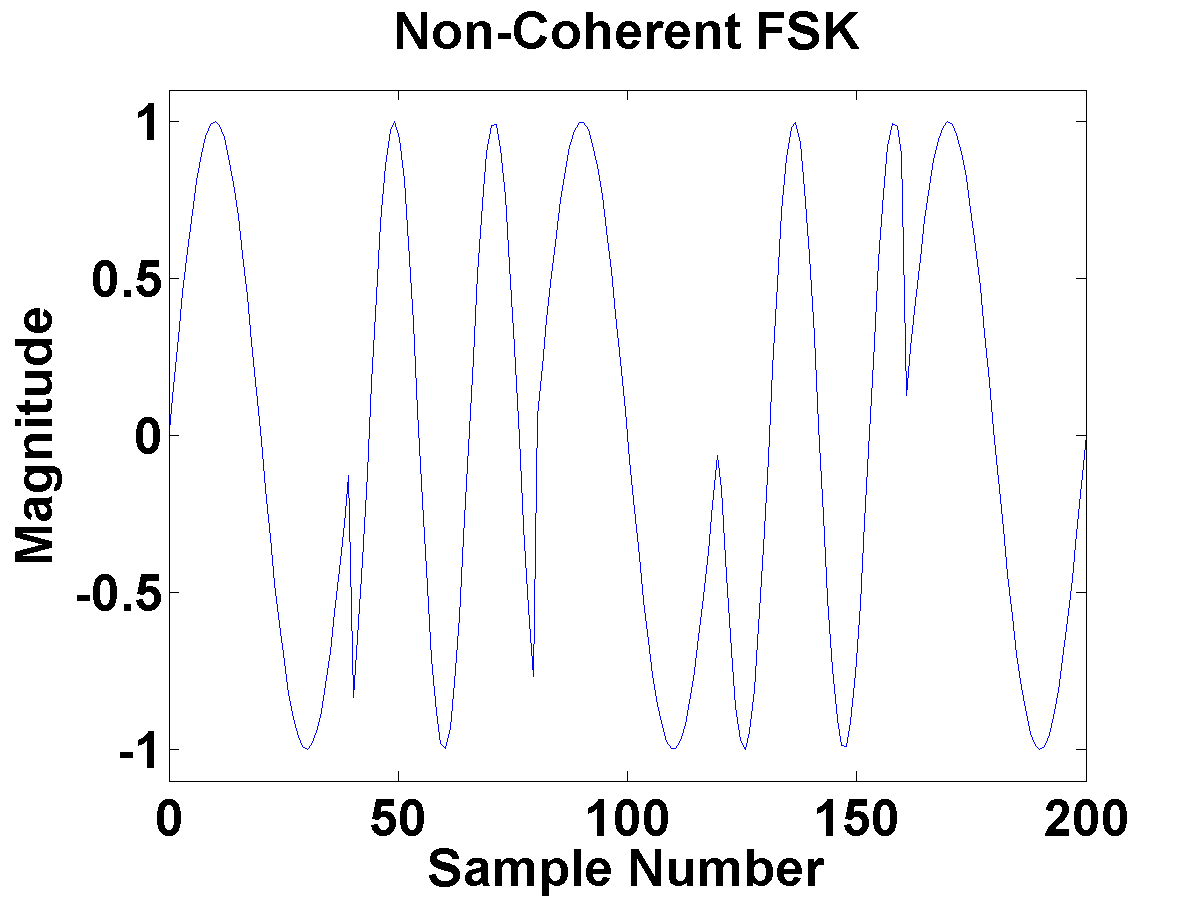
\includegraphics[width=0.75\linewidth]{images/NonCoherentFSK.png} 
	\caption{Example of a non-coherent 1200Hz / 2200Hz FSK signal.}
   \label{noncoherentFSKExample}
\end{figure}
\begin{figure}
  \centering
	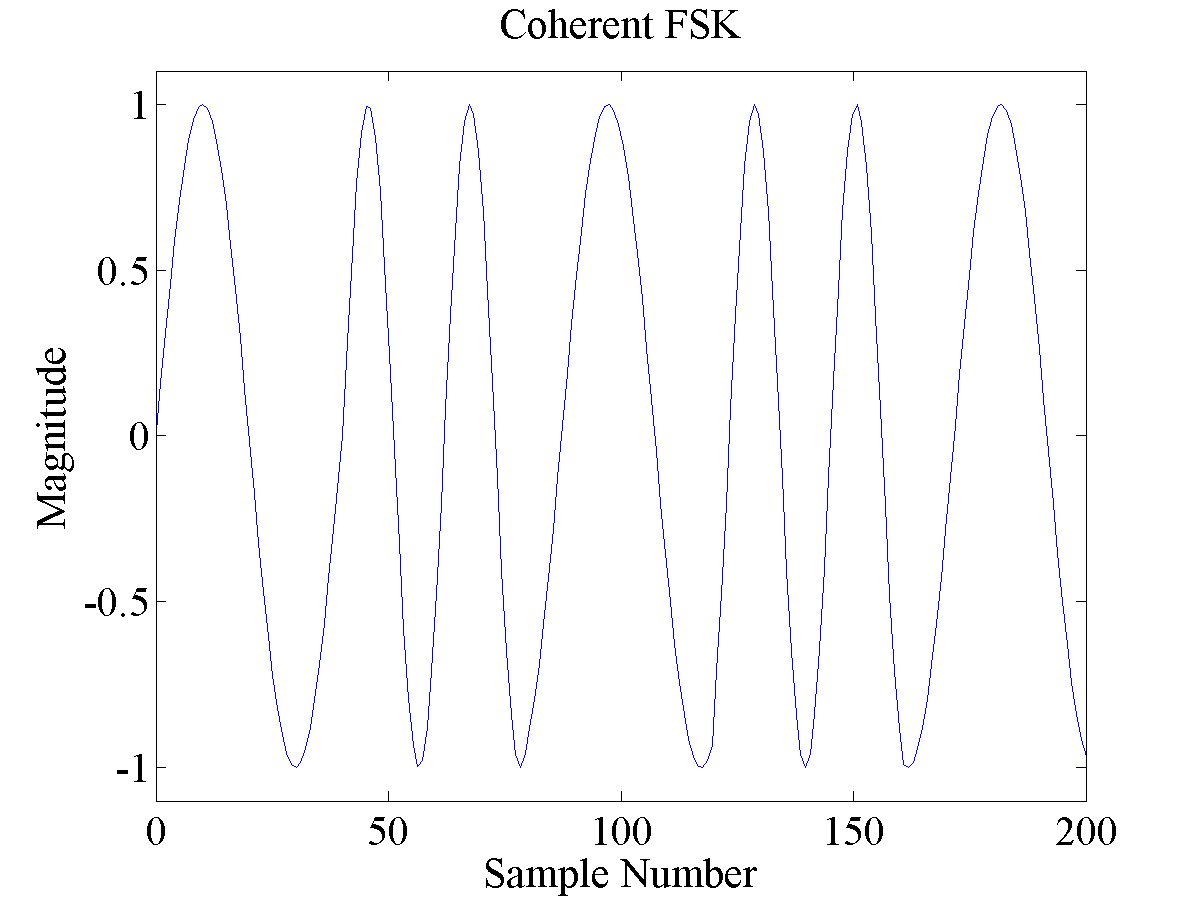
\includegraphics[width=0.75\linewidth]{images/CoherentFSK.png} 
	\caption{Example of a non-coherent 1200Hz / 2200Hz FSK signal.}
   \label{coherentFSKExample}
\end{figure}

\section{Zero Crossing}
Using zero crossings to determine the frequency of the FSK signal is one of the the easiest algorithms from a software implementation perspective. The idea is that based off of the time elapsed between zero crossings of the signal the period of the waveform can be measured. Once the period has been calculated the frequency can then be easily calculated using the inverse relationship between period and frequency, \textit{f} = 1 /T where \textit{f} is the frequency and T is the period. It is worth noting and keeping in mind that two consecutive zero crossings are only half of the period since there are a total of three zero crossings in one period.

\section{Correlation}
Another method that can be used for demodulation of FSK is correlation with the underlying FSK signals. For APRS this is done by synthesizing a 1200Hz tone and a 2200Hz tone and then comparing the input signal to each of these. Which ever one of the synthesized signals the input signal is more similar to - has more correlation with - the input signal must be the frequency that is present at that point in time in the data carrying signal. 

\section{Discrete Fourier Transform}
A discrete Fourier Transform is one implementation of Fourier Transform that is executed on discrete samples similar to what is present in a digital audio file. Once a Fourier transform has been applied on a signal the output is a relative power versus frequency. With this data which ever frequency, either 1200Hz or 2200Hz, is more prominent is which symbol must be present in the bit period.

\subsection{Goertzel Algorithm}
Computing a discrete Fourier transform is more reasonable computationally than a full Fourier transform which is an integral as opposed to having discrete terms \cite{WikipediaFT}. However, even the results from the DFT could have more data than is needed to do the demodulation since the results will be a spectrum of powers over a range of frequencies \cite{WikipediaDFT,WikipediaFFT}. A more simplified and specified approach can be used. The Goertzel Algorithm evaluates the coefficients and corresponding powers of the individual frequencies of 1200Hz and 2200Hz \cite{WikipediaGA,Elmenreich2011}. 

\section{Phase Lock Loop}
A phase lock loop (PLL) is exactly what the name implied. It is a loop that stays locked onto the phase of the input signal. This is done by taking input signal detecting the phase and then producing an output the corresponds with the phase. The output is fed back in with the input so that any differences between the input and output of the phase lock loop can be reconciled to have a phase exactly in phase with the input. The convenient thing about monitoring the phase of the signal so closely and being able to stay locked onto it is that the frequency must also be known. Extracting this frequency information from the PLL can hence be used for FSK demodulation.

\section{Advantages of Using the Derivative of the Original Signal}
One thing considered while trying to demodulate the Bell 202 signals was the implications of using the derivative of the signal for decoding as opposed to the actual signal. One advantage that was seen through using this approach is that for cases where there is a DC offset of the signal, the derivative would remove this and re-center the signal about zero. A consequence of using the derivative of a sine wave signal is that the result will be 90 degrees out of phase. It was decided that this would not be a problem since the whole signal would be 90 shifted by this amount and the timing is done on the fly once the signal is received anyways. However, there were some other things about using the derivative that were not considered until later. One thing is that in addition to to helping the DC offset it also helps signals that were de-emphasized by not pre-emphasized. In signals where this is the case the 2200Hz tones will be lower in the original signal, but since they have a steeper slope this ends up helping to normalize these differences in the resulting derivative. An example showing this problem as well as a DC offset in the data signal and its derivative can be seen in Figure \ref{emphasisAndDerivativeExample}. Although the derivative helps with this, it will hurt if the opposite is the case (preemphasized but not deemphasized) only worsening the problem.
\begin{figure}
  \centering
	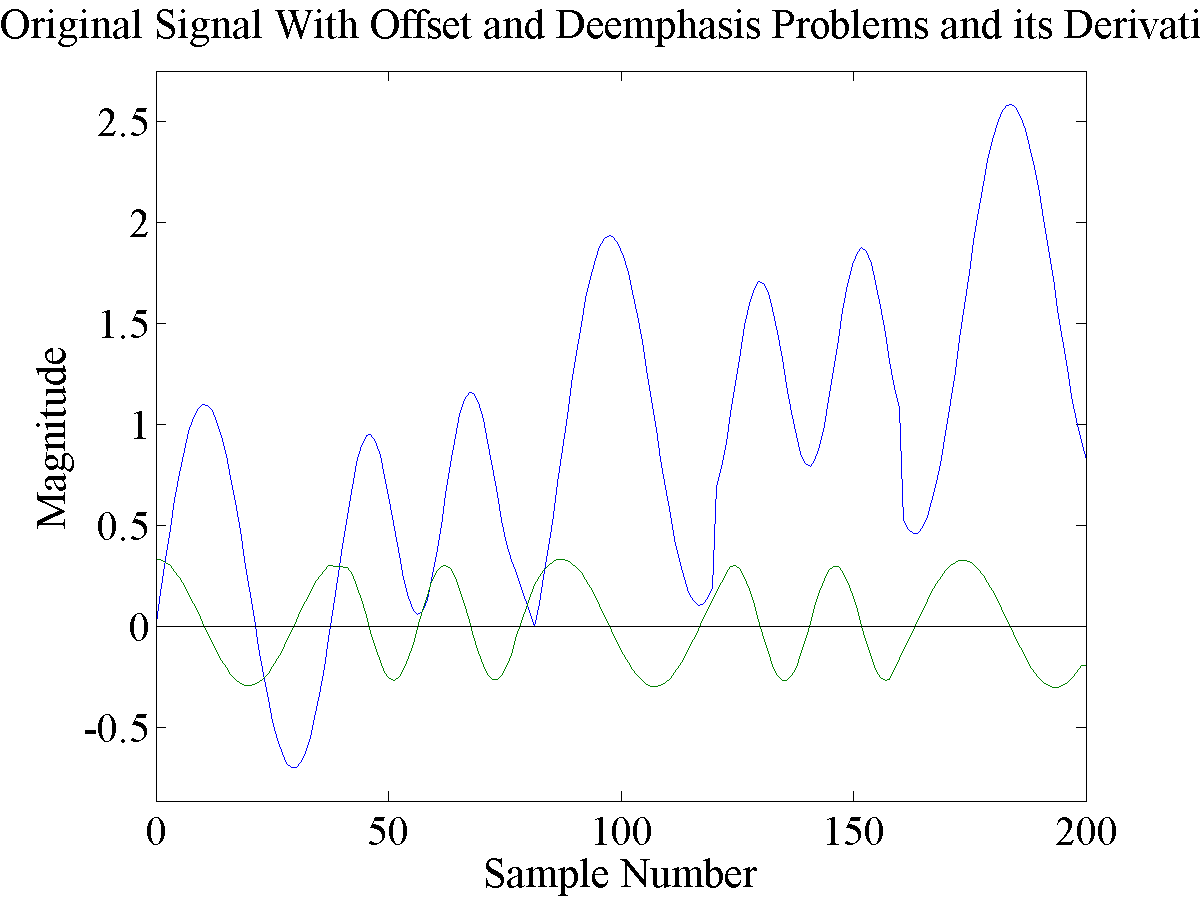
\includegraphics[width=0.75\linewidth]{images/OriginalSignalWithOffsetandDeemphasisProblemsanditsDerivative.png} 
	\caption{Example of a signal that has both a DC offset and a deemphasis problem and its corresponding derivative.}
   \label{emphasisAndDerivativeExample}
\end{figure}

\section{Additional Benefits of Software Based Decoding}
Software is flexible. Any one of the aforementioned algorithms can be used on the same hardware without having to add additional discrete components, add new Integrated Circuits (ICs), or make modifications to a Printed Circuit Board (PCB). There are a two benefits of using software instead of dedicated hardware that this research will investigate; first exhaustive search of a signal through the use of buffers, and second, the ability to be able to run multiple of these demodulation approaches in parallel.

\subsecion{Exhaustive Search of Incoming Signal}
Using software the input signal can be buffered in the program and then searched for a signal. Since there is not a separate data and clock signal, there could be a case when the clocking is improperly selected. Using an approach of buffering data that may contain a valid packet, the software can step through the data trying every possible clocking option.

\subsection{Taking Advantage of Parallel Demodulation}
Another potential advantage of using software for decoding these AFSK signal is being able to apply multiple demodulation techniques. Once the data is collected in coverted to a digital form there is no reason, other than computation limitations of the host computer, not to run multiple algorithms in parallel in order to be able to demodulate the maximum number of packets possible. Although there are packets that every algorithm is able to decode, there are also those that some approaches can decode while others can not. Through using multiple in parallel for demodulation and de-duplicating the demodulated results even more packets can be correctly decoded.

\chapter{Demodulator Benchmarking}
In order to compare the results of the different demodulators a method of benchmarking must be instituted. Each one of the demodulators was tested using multiple audio files that have different characteristics. These different files as well as the advantage of using them in the benchmarking are explained in their corresponding section. It is worth noting that for each test audio file a sample rate of 48000Hz was standardized on since it works out nicely to 40 samples per bit period for 1200 baud digital communications. Although all the tests were performed with audio at a sample rate of 48000Hz, it is not expected that the results would change much if a different sample rate was chosen since items are calculated from file meta data as opposed to hard coded constants to suite 48000Hz audio.

\section{Plain, Straight, and Clean Packets}
These audio files were just what the title implies - straight packets. What is meant by straight packets is that they are pure "perfect" 1200Hz and 2200Hz tone audio samples. There is no noise introduced through artificial or natural means such as noise introduced through the intrinsics of using RF and the medium. Although these files do not provide meaningful results for hardware or already implemented software solutions (since these devices will be able to decode every packet in the audio file) it still provides a good starting point for getting new algorithms up and running. Two of these clean files were generated. One was generated from an OpenTracker creating packets with a counter and the text "The quick brown fox jumps over the lazy dog". This audio file contained a total of 40 packets and proved to be short enough to allow for quick cross checking as modifications were made. The second file was generated in software using Toledo's javAX25 package. All that is relevant at this point is that it has perfect levels (1200Hz and 2200Hz tones are at the exact same level) and contains 200 packets making the file quite a bit longer. An example segment from the 200 packet audio file can be seen in Figure \ref{gen200Segment}.
\begin{figure}
  \centering
	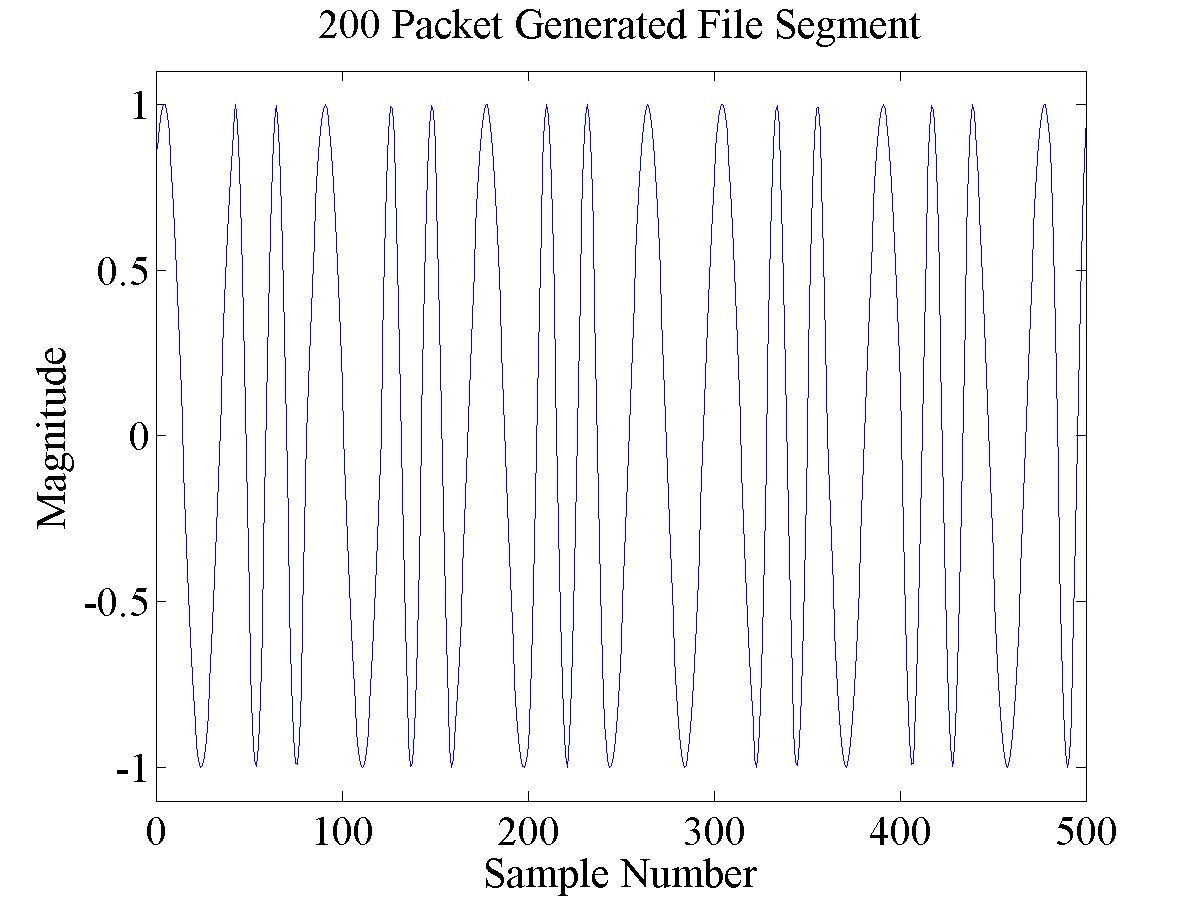
\includegraphics[width=0.75\linewidth]{images/200PacketGeneratedFileSegment.png} 
	\caption{Example of the AFSK present signal in the 200 packet generated file.}
   \label{gen200Segment}
\end{figure}

\section{White Noise Testing}
The second test file that was used on the demodulators was the 40 packet OpenTracker file mentioned in the previous section with added artificial white noise. An advantage of this file is that its contents are known while still being a reasonable benchmarking file. No demodulator could demodulate all the packets out of the file as the noise was increased all the way up to a signal to noise ration (SNR) of 0.5. There were total of 10 steps of increasing noise meaning that at each noise level there were approximately 4 packets. This noise was added to the original audio file using the audio editing program Audacity \cite{Mazzoni}. Although this file does not directly characterize what is introduced by RF, it provides a reasonable test simulating the effects of a decreased SNR on the audio signal. An example segment from this white noise added file can be seen in Figure \ref{OT3TestwNoiseSegment}.
\begin{figure}
  \centering
	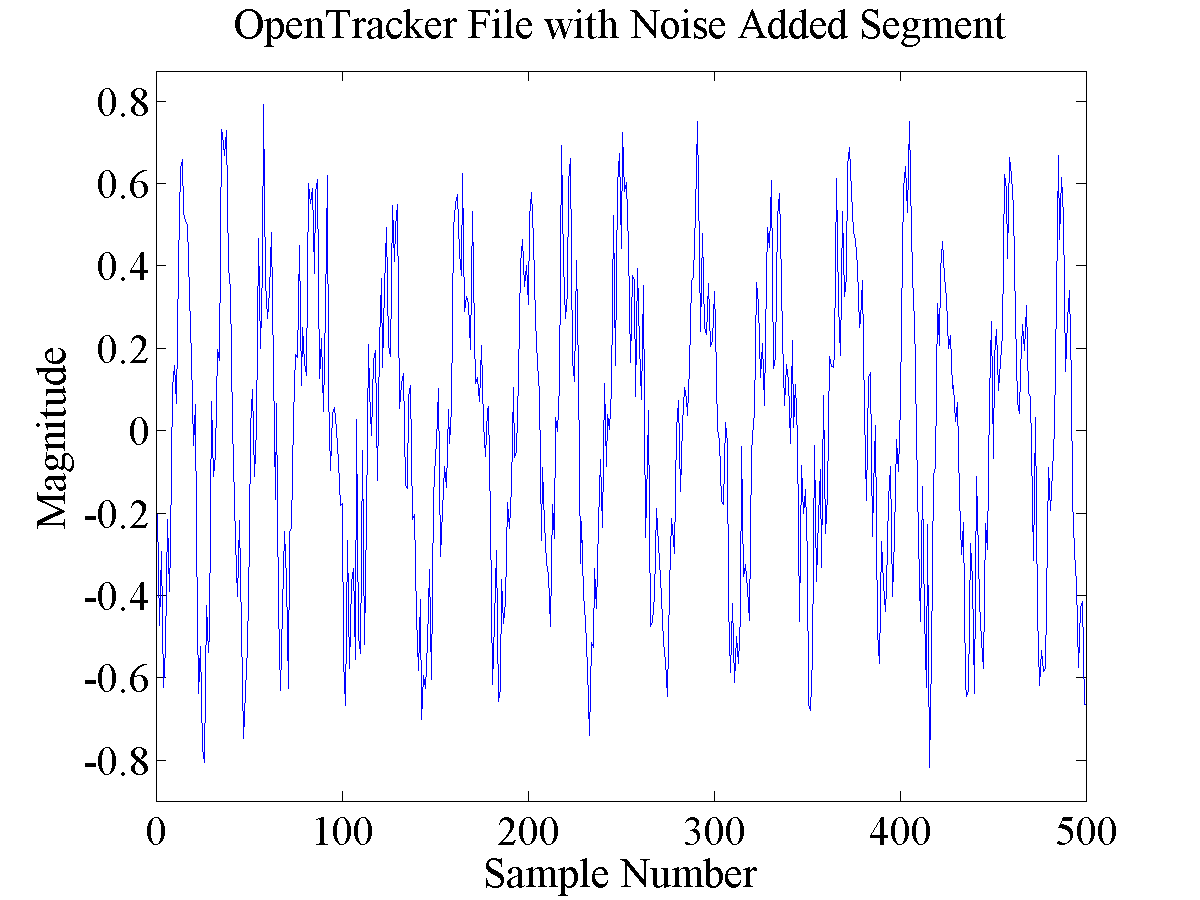
\includegraphics[width=0.75\linewidth]{images/OpenTrackerFilewithNoiseAddedSegment.png} 
	\caption{Example of a generated AFSK signal with artificial white noise added.}
   \label{OT3TestwNoiseSegment}
\end{figure}
 
\section{Los Angeles APRS Test Recordings}
%:04-25:45 57/min averaging over the first 3 minutes
This next benchmark is the de-facto benchmark for demodulators. The idea behind it is simple, yet it provides a very comprehensive test. The author of this file recorded on air APRS traffic in the Los Angeles Area for 45 minutes. He then removed segments of no traffic and condensed 45 minutes of live recording down to about 25 minutes \cite{Smith2009}. The nice thing is that it is real traffic which contains all of the real life situations including stations close to the receiver, far from the receiver, moving, stationary, different transmit power levels, different hardware, and varying content just to name a few. One disadvantage is that since it is just a random recording of traffic on the air, there is no definitive answer of how many packets are in the file. After listening to the audio file by ear it is approximated that there are a total of about 1463 packets by listening to the first 3 minutes as a sample and extrapolating to the length of the audio segment. This is considered \textit{the} file use for benchmarking in the community and when people discuss the performance of their demodulator, they quote it in how many packets they were able to successfully decode out of this file. An example segment from this off air recording of APRS traffic can be seen in Figure \ref{Track1Segment}. This is just one of the audio files on this author's test CD and is in fact the first one on the CD, so it will be referred to as Track 1. This was the the file that was most important to the testing, but the author also has a second version of this file in Track 2. The only difference between Track 1 and Track 2 is that an audio filter was used to create Track 2 which had the result of being a deemphasized version of Track 1. 
\begin{figure}
  \centering
	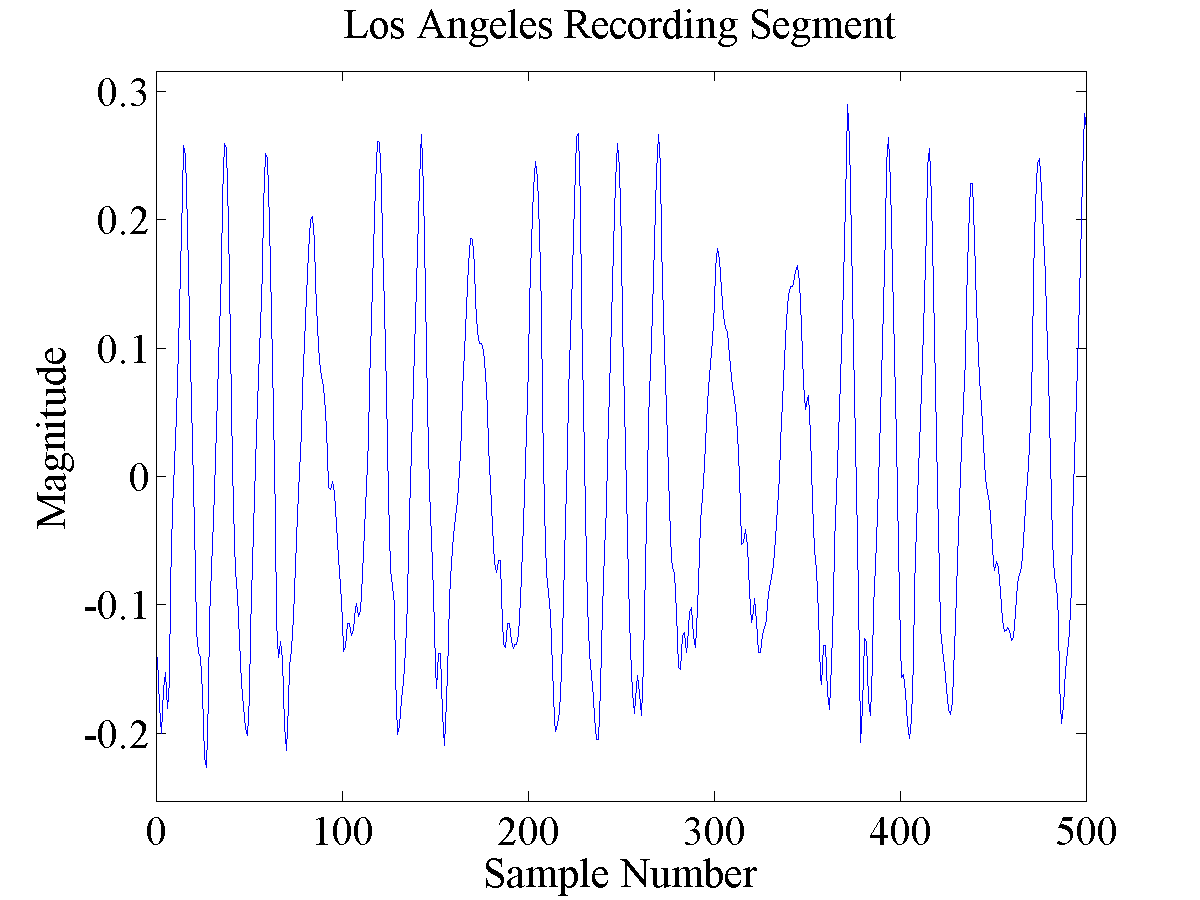
\includegraphics[width=0.75\linewidth]{images/LosAngelesRecordingSegment.png} 
	\caption{Example of the AFSK present signal in Track 1 of the Los Angeles Recording Test File.}
   \label{Track1Segment}
\end{figure}

\chapter{javaAX25}

Another software based demodulator that is available is Sivan Toledo�s JavaAX25 software package. The advantage of using this package for benchmarking different algorithms is that due to his code structure and package hierarchy it makes it simple to change different demodulation algorithms. The software is hosted on github making it convenient to access the repository. The next few paragraphs will give an overview of the features that Toledo�s software package has available in it \cite{Toledo2012,javax25github}.

JavaAX25 is a comprehensive package for doing software based modulation and demodulation of APRS packets. It includes packages for interfacing with radios, sound cards, and other standard packet programs that are used on computers; one such example is that there is a plugin to be able to use JavaAX25 with AGW Packet Engine. In addition to having all of the items that are needed to be able to do the AX.25 modulation, demodulation, and interfacing with hardware, there is also a testing framework.

From within the testing framework each aspect of the software suite can be tested. The three portions that were used most extensively in this research were the modulator, demodulator, and testing framework. In order to have a demodulator one needs to have it be a child of an abstract class that implements methods for adding individual samples to the algorithms for processing, checking to see if the current signal might be a data carrier, etc. Due to the fact that the data flow was very clear for the demodulators it made it simple for different demodulators to be implemented and then tested using the �Test� class.

The main method that is called by the class using the demodulator in order to pass the data to the algorithm is the addSamplePrivate method. This method is a way for the calling class to give data to the algorithm to be processed. Each sample is a value that corresponds to the magnitude of the audio signal at that instant in time. The samples themselves derive from the fact that digital audio is sampled at a given sample rate. For this research sample rates of both 44100 and 48000 were used, but 48000 samples per second was standardized on since it divides evenly into 40 samples per baud on a 1200bps digital encoding. The goal of demodulators it to determine when a symbol transition has occurred, once this has been determined, the time elapsed since the previous transition is used to determine how many symbols have occurred. Since consecutive symbols represent a 1 bit, the number of symbols minus one will be the number of 1 bits to add to the packet followed by a zero.

The algorithm that Toledo is currently using for the demodulation is correlation based. This is done by correlating the input signal with both a 1200Hz and a 2200Hz sine wave and seeing which of the two the input signal correlates with more. Once the correlation with each is established he filters the correlation data in order to smooth the results and make it easier to be able to pull the correct frequency out of the calculations. However, before doing any of the correlation calculations the data is passed through a band pass filter centered about 1700Hz which can be seen in Figure 2.

\chapter{Implementation}

The implementation started with a naive approach that allowed for more insight to be gained into the JavaAX25 software package. Some of the results and features that were found have been presented in the previous section. The first algorithm implemented was a Modified Zero Crossing Algorithm explained in section 4.1. Section 4.2 discusses our strict zero crossing. Section 4.3 discusses the windowed zero crossing. Section 4.4 discusses the peak detection algorithm. Our final implementation is a Preclocking demodulation algorithm and is discussed in section 4.5.

\section{Modified Zero Crossing}

As the first implementation there were some assumptions that were made that worked as a disadvantage to the demodulation. The thought behind this algorithm was to set a threshold around zero and when the value rises above this threshold centered on zero or falls below, determine that a zero crossing occurred. The time between subsequent zero crossings can be calculated in terms of the number of samples and the sample rate of the incoming audio can be used to figure out the time between the zero crossings in seconds.

One can calculate the time between zero crossings by realizing that they happen every p radians or twice in one frequency period. The period T can be calculated using T = 1 / f where f is the frequency. Using this information and the knowledge that the two tones are 1200Hz and 2200Hz one should expect zero crossings every 833�s and 455�s respectively. This logic of extrapolating the frequency from the zero crossing spacing of the signal is used for this as well as the next two algorithms presented in sections 4.2 and 4.3.

Upon implementing this algorithm there was an apparent disadvantage to using the threshold around zero. The original thought with this threshold is that it would help to get rid of erroneous zero crossings caused when there was low level noise on the signal. However, this buffer was not at all helpful since it doubled our opportunity for error on a zero crossing. If there was noise on the signal both right before entering the threshold and right before exiting this threshold it allowed for two separate contributions to error on figuring out exactly what sample number the crossing was at. Noticing this flaw the next algorithm, called the strict zero crossing, is exactly as the name implies; a strict zero crossing demodulation algorithm instead of having a threshold around zero.

\section{Strict Zero Crossing}

The strict zero crossing algorithm had advantages over the initial zero crossing algorithm implemented since it only has one area where error can occur. Unlike the algorithm in section 4.1 the zero crossing corresponds to exactly one value sample as opposed to relying on two samples in order to the back calculate the zero crossing.

The initial algorithm kept track of whether the signal was high (above zero) or low (below zero) and then when it transitioned to the opposite this was considered a zero crossing. The spacing between crossings was then used to calculate what frequency must be present in the signal using the logic explained in section 4.1. The initial results for this algorithm were good with clean signals, but once any noise was introduced, it still suffered from the same problems as the first Zero Crossing algorithm which was that the noise was bumping the zero crossing values around.

One example of the zero crossing weakness to noise was having 1200Hz tones that looked like 2200Hz tones. This case arose when the noise made one of the 1200Hz crossings happen a little late and then the subsequent zero crossing for the 1200Hz crossing a little early. This now smaller time between what should be a 1200Hz crossing distance now instead looks like a 2200Hz tone. In order to alleviate some of the trouble caused by this random white noise some filtering was added. See Figure 3 for an example of noise corruption.

At first the filtering chosen was just an average of the two adjacent points. This had better results for some cases, but not for all. For instance, if the noise was just affecting one zero crossing used for the calculation of the frequency it helped, but if the noise was affecting both zero crossings that were needed to figure out the frequency then we found that moving up to an average of three points proved to have the best results in terms of total number of packets decoded. This does makes sense though since if the noise causes the signal to jump either above or below the true value and averaging the three adjacent points allowed for two of them to be very noisy and cancel each other out while still having one to keep the filtered value from the averaging as close as possible to the original signal.

In addition to doing a straight averaging of the three adjacent points, some effort was put into doing a weighted average. The results from the weighted average were not as good since the whole point was to try and filter out some of the noise. If specific points were weighted instead of doing the unweighted average it meant that the goal of the filtering through averaging was useless. This is because if more weight is put on any one of the value it means that the noise in that point could overwhelm the calculation, and as mentioned then throw off the point of the filtering which is to get a closer approximation to the original signal value.

\section{Windowed Zero Crossing}

Although the strict zero crossing was much better than the original zero crossing algorithm there were still improvements that needed to be made. The filtering that was done through averaging adjacent points helped, but in some extreme cases it was still not enough. The next algorithm relied on averaging the averages. Basically instead of just looking on a crossing to crossing basis, a sliding window about the length of a symbol period is used, and the crossings within that window counted. The thought was that this would place less dependence on each zero crossing being calculated correctly since it is only one data point and hopefully the other one or two in the window will make correctly determining the frequency of the tone present in the signal more accurate. 

In order to make it more deterministic how many crossings were expected in the window a window size slightly less than one baud was chosen. The reason for this is that for a 1200Hz tone if the size of the window is just one sample greater than a symbol period there may be 3 crossings in the window since the signal is 1200 bps and hence the 1200Hz tone can complete one full period during the time elapsed in one symbol period. Making the window slightly less, 90% the size, than the symbol period ensures that noise will not interfere with the crossing count and that within the window there will only ever be 2 crossings if a 1200Hz tone is present in the window. If there are less than two crossings in the window then there is just noise / a DC offset and greater than 2 crossings is assumed to be a 2200Hz tone. This may seem like a far leap, what if there is noise at 20,000Hz? This was handled by requiring a minimum time to elapse between crossings that was a little less than that expected for subsequent 2200Hz crossings. This does mean that the algorithm will favor 2200Hz tones over 1200Hz tones when in the noise, but it still picks up the 1200Hz tones fairly well.

This theory and approach is all fine and dandy up until actually applied. Although, it originally seemed like a good idea, there were problems with setting all the values �correctly.� For instance there are three apparent variables that can be tweaked in order to change the performance: 1. the size of the window, 2. how many crossings should be expected within the selected window size, and 3. the amount of time to wait before allowing a zero crossing the be considered a zero crossing. Modifying these three parameters showed many different results in terms of the total number of packets decoded by the algorithm. For instance in the Open Tracker 3 test file that had 40 packets in it (more information on it in section 5) the algorithm could decode 39 of the packets with the window size set to 90% of a symbol length and the number of successfully decoded packets would drop if the window size was decreased below 87% or increased above 93%.

\section{Peak Detection}

The peak detection demodulator was developed to try and mitigate some of the problems observed with the strict zero crossing method. This takes advantage that peaks will occur on exact sample intervals while zero crossings samples don�t typically don�t occur directly at the crossing. This delay for the zero crossing can lead to ambiguity by a sample or two on either side of the zero crossing. The number of samples between the zero crossings can be either expanded or compressed by a few samples causing misidentification. By using peak detection this ambiguity could be further reduced. 

The algorithm uses the absolute value of the time domain to move the troughs to be peaks so transitions can be detect if they occurred during the peak to trough transition using the peak algorithm.  A three sample average is used for each incoming sample to help smooth the noise present. Three samples blends the noise while still preserving the integrity of the shape of the sinusoidal signal. The current sample is then compared to the previous local peak and stored if it�s higher along with the sample index number. If the two previous samples are consecutively decreasing a peak has occurred and the signal is moving in the downward direction. The handlePeakDetection() method is then called and after processing is completed the resets the local peak, local peak index, samples since the previous peak, and moved into the decreasing state. While in the decreasing state, the algorithm determines if the state has changed to increasing when three consecutive samples are larger than the previous. Once the increasing state has been entered, the algorithm repeats waiting for a peak.

The handlePeakDetection method first determines the number of samples between the current and previous peaks. This value is then subtracted from the previous number of samples between peaks. If the difference is greater than a threshold a transition has occurred. Once a transition has been detected, the number of bits is determined and the previously mentioned packet creating process in the JavaAX25 documentation is utilized.

The peak detection demodulation method was able to detect extremely clean source signals, but struggled against real world signals. It was difficult to tweak the algorithm to decode packets. Changing the difference threshold would help in some cases, while hurt in others making no perfect solution. Many packets had only a few bit errors. This approach could maybe be improved by averaging the previous peak periods to more clearly determine a transition occurrence, but due to time constraints more effort was put into the next demodulation technique. 

\section{Preclocking Demodulation}

Using the information collected thus far and the now greater knowledge of the software package as a whole the next algorithm is considerably more complicated. There are size different steps to the algorithm. First, filter the data to remove noise and higher frequency components and make the signal smoother. Second, look for flags in the signal so that the demodulation can happen one packet at a time instead of just blindly trudging forward through the packet sample by sample. Third, take the derivative of the whole packet to and determine the zero crossings. Fourth, frequency transitions are extrapolated from the derivative data. Fifth, the frequency transitions of the packet clocking are calculated and finally, sixth the tone demodulation is done on a baud by baud basis.

The original goal with this much more complicated algorithm than its predecessors was to take advantage of the clocking of the original signal. Using the clocking in the digitally encoded signal, more confidence can be instilled into making sure that every symbol gets demodulated correctly. The filtering and flag finding is done using the preexisting code that Toledo wrote, so not that many details will be included about it here. Instead the explanation of the inner working will start with why the derivative of the input signal was used. The nice thing about using the derivative in this algorithm instead of the original signal is that it solves two previously encountered problems: 1. the DC offset problem and 2. the emphasis problem. DC offset is when the oscillation of the frequency doesn�t occur around zero, but has been biased around a different DC voltage. This can occur in hardware due to the different strengths of the two signals. If a 1200 Hz tone has a higher magnitude than the 2200 Hz tone the 2200 Hz can be off centered on the voltage at the transition time. This can be observed in Figure 4. The Bell 202 signal is typically FM modulated onto a carrier for RF transmission and FM Modulation tends to attenuate higher baseband frequencies. In audio systems the higher frequencies are amplified before FM modulation and then attenuated after demodulation on the receiver. This creates a stronger 2200 Hz tone. There is no standard practice among amateur APRS users as to how/when to emphasis or de-emphasis packets. This creates the need diverse detection criteria to address the biasing of either 2200 Hz or 1200 Hz without knowing ahead of time which emphasis state has occurred. See Figures 5 and 6 for examples. Due to the nature of the derivative the DC offset problem is solved very literally, but solving emphasis problems is not necessarily as obvious, however it still shows improvements over the original signal. See Figure 7.

Once the data is filtered through both the direct FIR band pass filtering and through the derivative the frequencies seen in the packet are stored and using linear interpolation the exact point that each frequency transition occurred at is stored. Since frequency transitions will only happen along baud borders this allows for the clocking to be extrapolated from these transitions. The clocking is then determined in terms of offset in samples from the start of the possible packet. This is done through going through each one of the possible clockings (for a 48000 sample per second audio source this works out to 40 possible alignments) and selecting the sample offset number that minimizes the square distance between that perceived clocking and the observed transitions. 

Once the clocking is determined the frequency data that was calculated using the zero crossing from the derivative is used in order to figure out the actual tone that is contained within each baud. Two different approaches were tried to extrapolate the frequency out of the symbol window. First it was thought that taking the average of each one of the frequencies that fall within the baud period that just calculated would be best, but it became apparent that the filtering and derivative was not enough. Within decoding of legitimate packets frequencies greater than 5,000Hz were detected skewing the 1200Hz tones to look like 2200Hz when averaged. Another approach of just taking the one value directly in the middle of a baud period was used, but this didn�t prove to be worse. The minimum amount of time to pass between zero crossings in the algorithm was modified to try and get more accurate frequency results. Then the detected symbols were histogrammed to see how many determined frequencies were ambiguous between 1200-2200Hz. The result showed a clear division between the two frequencies and the threshold was set in the middle at 1700 Hz for the average of the frequencies inside the baud period as seen in Figure 8. The end results explained in more detail below show prove that this algorithm is on par with the original correlation algorithm and can decode some packets that it could not.

\chapter{Testing}
In order to be able to evaluate the results from this research, each demodulation technique considered needs to be tested and the number of packets that each technique was able to successfully decode needs to be compared. From this analysis, it will be seen which techniques are effective and are able to decode relatively more packets as opposed to those that decode fewer. In order to validate the techniques results for dedicated hardware will also be collected for comparison. The testing for both the dedicated hardware and the software algorithms will be described in the corresponding sections below.

\section{Hardware Testing Setup}
The testing setup for the hardware is fairly simple since they are basically black boxes that just need to be supplied with the correct inputs. Each piece of hardware has two connections; one is the radio port, and the other is the serial connection. As the name implies, the radio port is used to be able to interface with the radio. This port has connections such as transmit audio, receive audio, push-to-talk (PTT), supply voltage (VCC), and ground. A digram of the common radio port can be see in Figure \ref{RadioPortPinout} and found in any manual including those of Argent Data\,\cite{Systems2013}. Since this was common between multiple pieces of hardware, a simple break-out board was created that allowed for a more universal audio transport mechanism of 3.5mm tip-ring-sleeve connectors, and also a 2.5mm barrel jack for power. This was much simpler than actually interfacing with a radio since the audio could just be played from a computer into the device; this device can be seen in Figure \ref{BreakOutBoard}. 

\begin{figure}
  \centering
	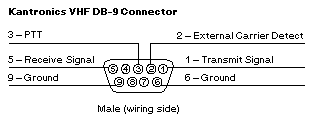
\includegraphics[width=0.75\linewidth]{images/RadioPortPinout.png} 
	\caption{Example Radio Port pin out for Kantronics, also consistent with others including OpenTrackers\,\cite{Martin2014}.}
   \label{RadioPortPinout}
\end{figure}
\begin{figure}
  \centering
	\includegraphics[width=0.75\linewidth]{images/BreakOutBoard.png} 
	\caption{Break-out board fabricated for hardware testing. There are two audio ports on the board; one for audio in and the other for audio out. On the right is the barrel jack fro supplying power.}
   \label{BreakOutBoard}
\end{figure}

\section{New javAX25 Demodulator Testing Framework}
Included within the javAX25 suite was a testing application that could both generate and decode packets. However, it was limited to only being able to specify one audio file and one demodulation algorithm. Using this test file as a basis, a new testing application was created that allowed for the multiple demodulators to be compared side by side against multiple audio files with a single run of the application. In addition to the output being printed to the console, the output was also saved to a file. Having these features in the testing application allowed for a much more streamlined analysis of all the algorithms collectively and tuning individual algorithms. One very convenient aspect of programmatically testing is that it is very easy to add a loop to try a range of tuning parameters and then look at the results to decide what is the best option. All of the results listed in the following chapter are from the testing application and mechanism described here.

\chapter{Results}
This results chapter is meant as a mechanism to present all of the data that was collected on the performance of different demodulators. All of the demodulators that were tested in the course of this research will be shown, whether it be dedicated hardware or software. The first results that will be shown are those of the dedicated hardware, being TNCs and Argent Data's OpenTrackers. Following the hardware will be the software implementations. Following these two categories will be some general comparisons between them.

\section{Dedicated Hardware Results}
In the scope of this research a total of 12 pieces of hardware were tested. They include Argent Data's OpenTracker 2, OpenTracker 3, OpenTracker USB, OpenTracker 3 Micro, Kantronics Kam, two Kantronics Kam Plus, two AEA PK-88, a PK-232, a PK-232MBX, and an MFJ-1278. Hardware models for which more than one was tested will be differentiated by a number in parentheses following the model number. Please note that on the figures OpenTracker will be abbreviated OT.

The first two tests consisting of clean packets - 40 generated from the OpenTracker and 200 using Toledo's suite - was relatively uninteresting. Essentially every piece of hardware decoded all 40 and all 200 packets. The only anomalies to this were that the OpenTracker USB was only able to decode 39 and 193 out of the 40 and 200 packet files respectively. Additionally the OpenTracker 3 Micro missed one packet in the 200 packet file to only decode 199. Since there is no real way to debug and see the cause of decoding relatively fewer or more packets just the data for these hardware items is presented as it was measured to allow for comparison to the software. This will continue to be the case for the remainder of this hardware section.

Following the two easy files the next file is same content as the file with 40 packets in it, with the only difference being that noise was progressively added. In Figure \ref{allHardwareOT3Noise}, the two PK-88s stand out for being able to decode 25 of the 40 packets in this file.

 \begin{figure}
  \centering
	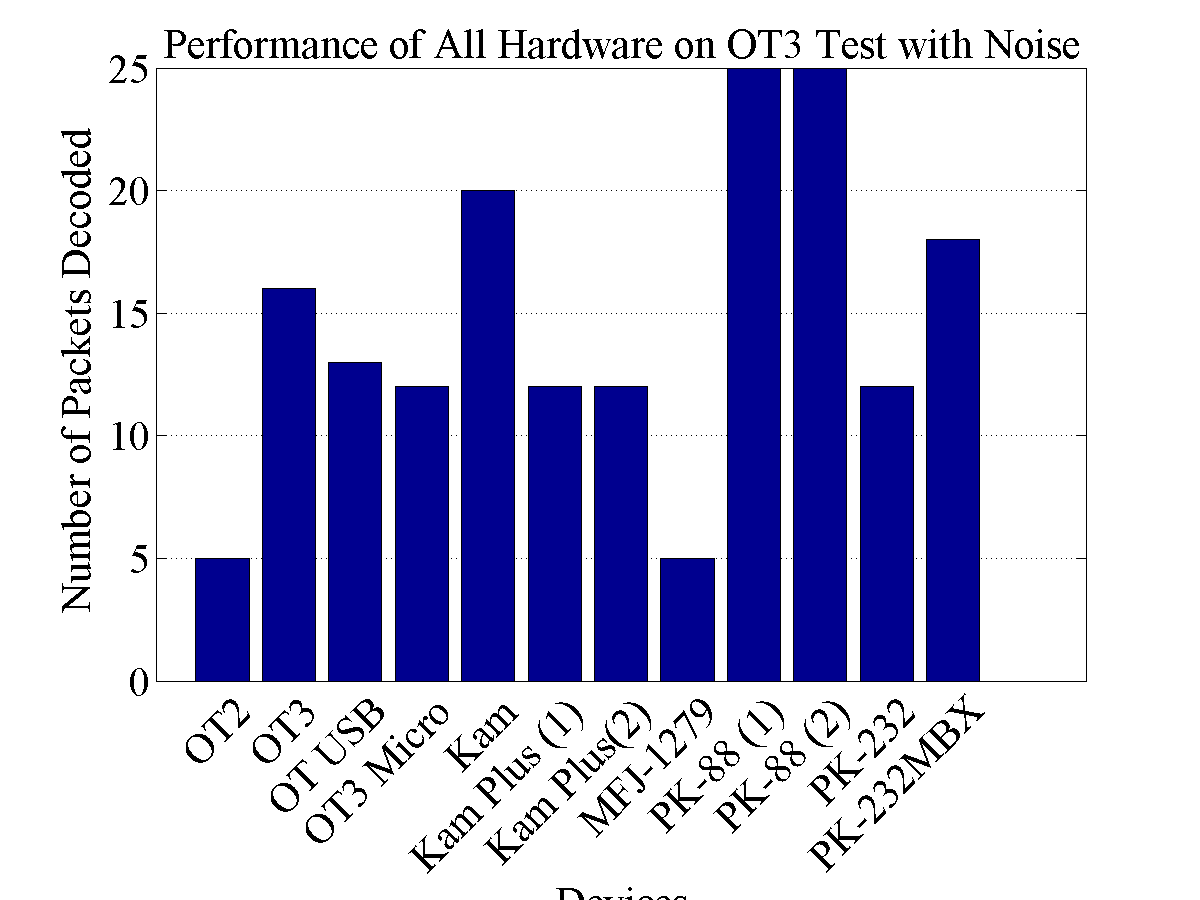
\includegraphics[width=0.75\linewidth]{images/PerformanceofAllHardwareonOT3TestwithNoise.png} 
	\caption{Number of packets successfully decoded for all tested hardware on the OpenTracker 3 test file with noise.}
   \label{allHardwareOT3Noise}
\end{figure}

The next two files are the ones that were used most extensively in the testing for comparison and tuning. Primarily the first, which is just a recording of traffic off the air. They are Track 1 and 2 from the APRS CD mentioned in the Demodulator Benchmarking Chapter. The results from Track 1 are in Figure \ref{allHardwareTrack1} and Track 2 in Figure \ref{allHardwareTrack2}. The top three performances of the hardware on Track 1 were the PK-88 (2) with 1007 packets decoded, the Kam with 988 Packets, and the Kam Plus (2) with 985 Packets. For Track 2 the top hardware was the Kam Plus (2) with 998, the Kam Plus (1) with 967, and the Kam with 938.

 \begin{figure}
  \centering
	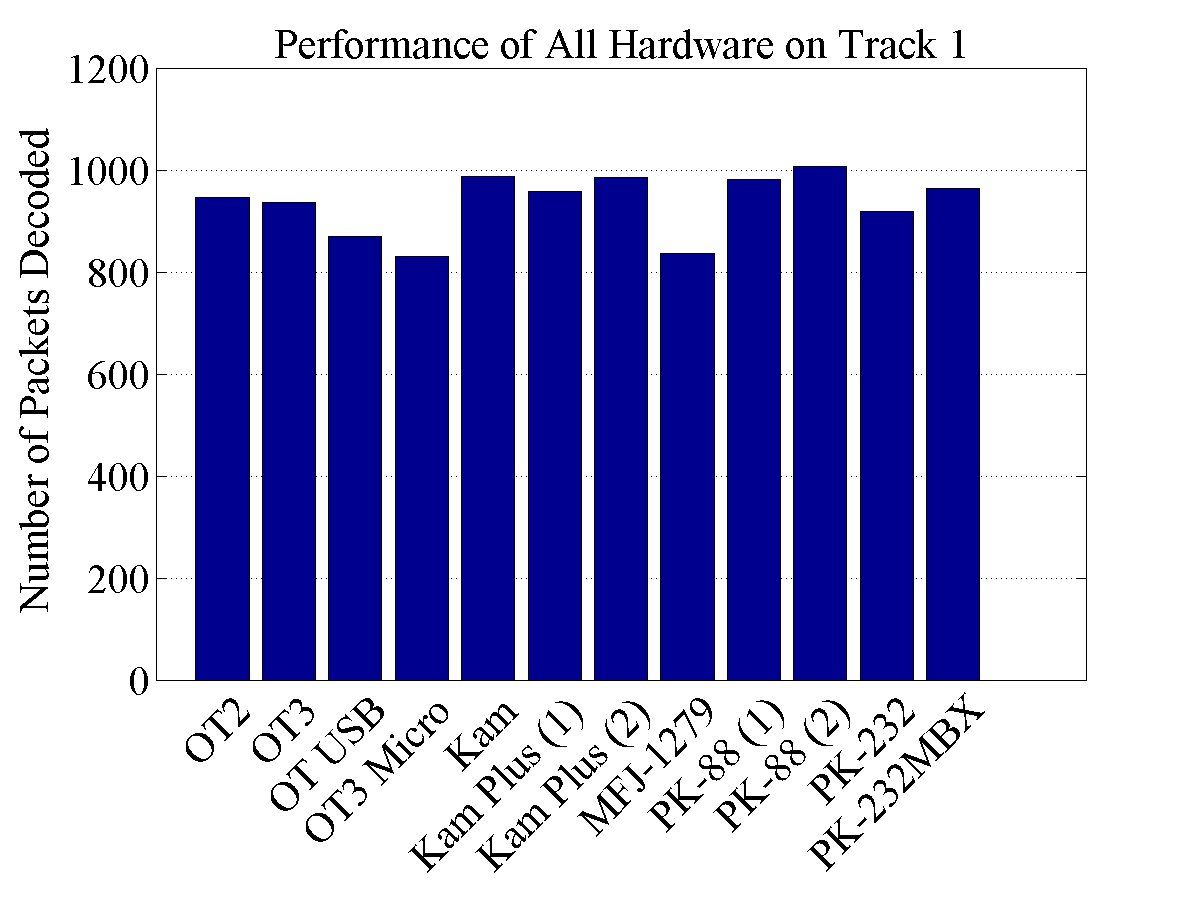
\includegraphics[width=0.75\linewidth]{images/PerformanceofAllHardwareonTrack1.png} 
	\caption{Number of packets successfully decoded for all tested hardware on the Track 1 test file.}
   \label{allHardwareTrack1}
\end{figure}

 \begin{figure}
  \centering
	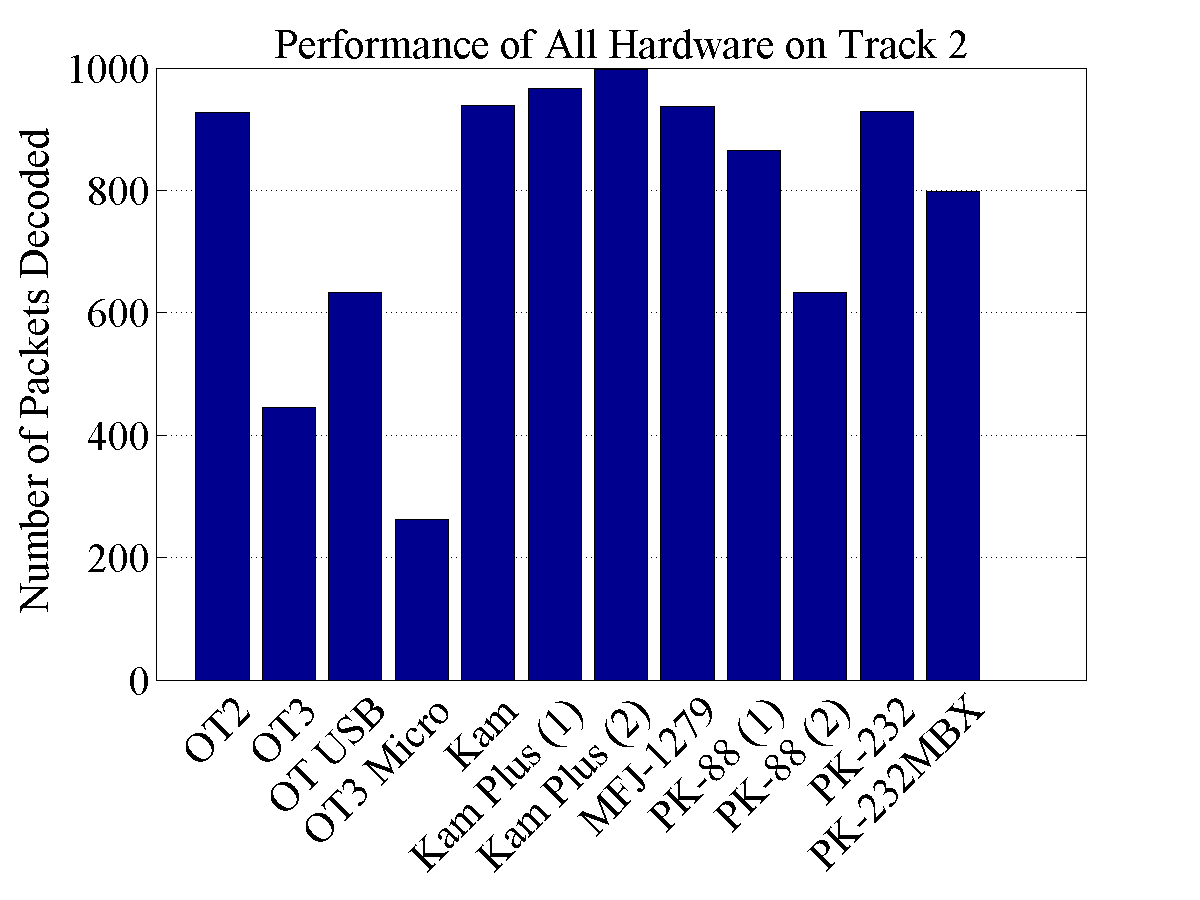
\includegraphics[width=0.75\linewidth]{images/PerformanceofAllHardwareonTrack2.png} 
	\caption{Number of packets successfully decoded for all tested hardware on the Track 2 test file.}
   \label{allHardwareTrack2}
\end{figure}

Using these results the best numbers for the hardware were 40 packets decoded from the Open Track 3 test, 200 from the javAX25 generated file, 25 from the Open Tracer 3 test with added noise, 1007 from Track 1 of the LA test suite, and 998 from Track 2. These best results can be used as a comparison for the software.

\section{Software Results}
In this section the number of packets that each of the demodulators in the javAX25 package was able to decode will be presented, highlighting those that were newly implemented in the course of this research. This will include the correlation approach that was already implemented before the start of this research as well as all of the new algorithms that were outlined in the previous chapter on Implementation. However, before getting the results from javAX25 there is one more data set to be introduced which is the results from another software based demodulation from AGW Packet Engine. Using this software 40 packets were decoded from the OpenTracker 3 test, 200 from the javAX25 generated file, 21 from the OpenTracker 3 test with added noise, 967 from Track 1 of the LA test suite, and 497 from Track 2. The results from javAX25 end up being on par with these results as well as those of the hardware.

With a total of 13 algorithms implemented, some did well and others not at all, so as in the section on hardware results, all of the data will be presented followed by a focus on those that performed the best. In the new javAX25 software implementation the filtering was moved from its original location of being on a per demodulator level basis to a central location that allowed each of the algorithms to utilize it. Some of the algorithms ended up relying on it after tuning and others could remain independent. As such, in order to present all of the data each algorithm will not only have a result for each of the 5 test files, but also for each of the three filters used on the data. The three filters used are no filter, a 900-2500Hz bandpass filter, and the same bandpass with a 6dB attenuation of 1200Hz tones to combat the signals that were not emphasized when transmitted but were deemphasized when received. For instance, for the Zero Crossing demodulator there will be three values for the OpenTracker 3 Test file, one at each filtering, and so on for the remaining 4 test files.

In terms of the data, correlation data will be on the far left of all the plots which was the current algorithm that it was the goal to beat. The performance of no filter on the OpenTracker 3 Test can be seen in Figure \ref{OT3FiltNo}, Figure \ref{OT3Filt0} shows data with the bandpass filter, and the emphasizing filter results in Figure \ref{OT3Filt6}. It can be observed that zero crossing did not favor the filters, others were resilient, and preclocking thrived. The Generated 200 Test file is the only file that the peak demodulator performed comperably to the other techniques on. The unfiltered data from this test is in Figure \ref{Gen200FiltNo}, the bandpass data in Figure \ref{Gen200Filt0}, and the results of emphasizing the signal in Figure \ref{Gen200Filt6}. Although the generated 200 packet file and the OpenTracker test file had similar results, the results for the generated 200 were better. This can be attributed to the fact that this file has only ever existed in the digital realm, it was made and consumed there, as opposed to existing in the physical world and then recording it.

\begin{figure}
  \centering
	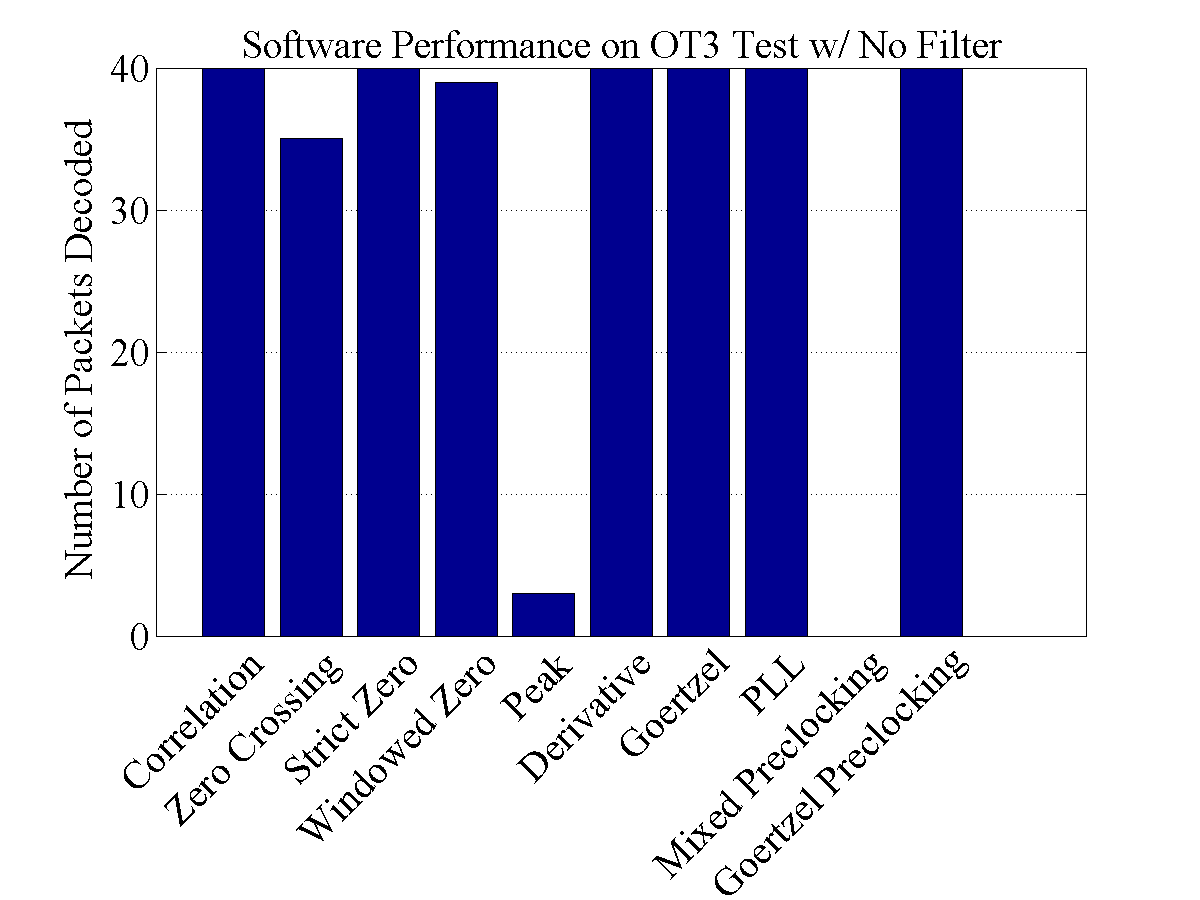
\includegraphics[width=0.75\linewidth]{images/SoftwarePerformanceonOT3TestwNoFilter.png} 
	\caption{Performance of software on the raw signal from OpenTracker 3 Test.}
   \label{OT3FiltNo}
\end{figure}
\begin{figure}
  \centering
	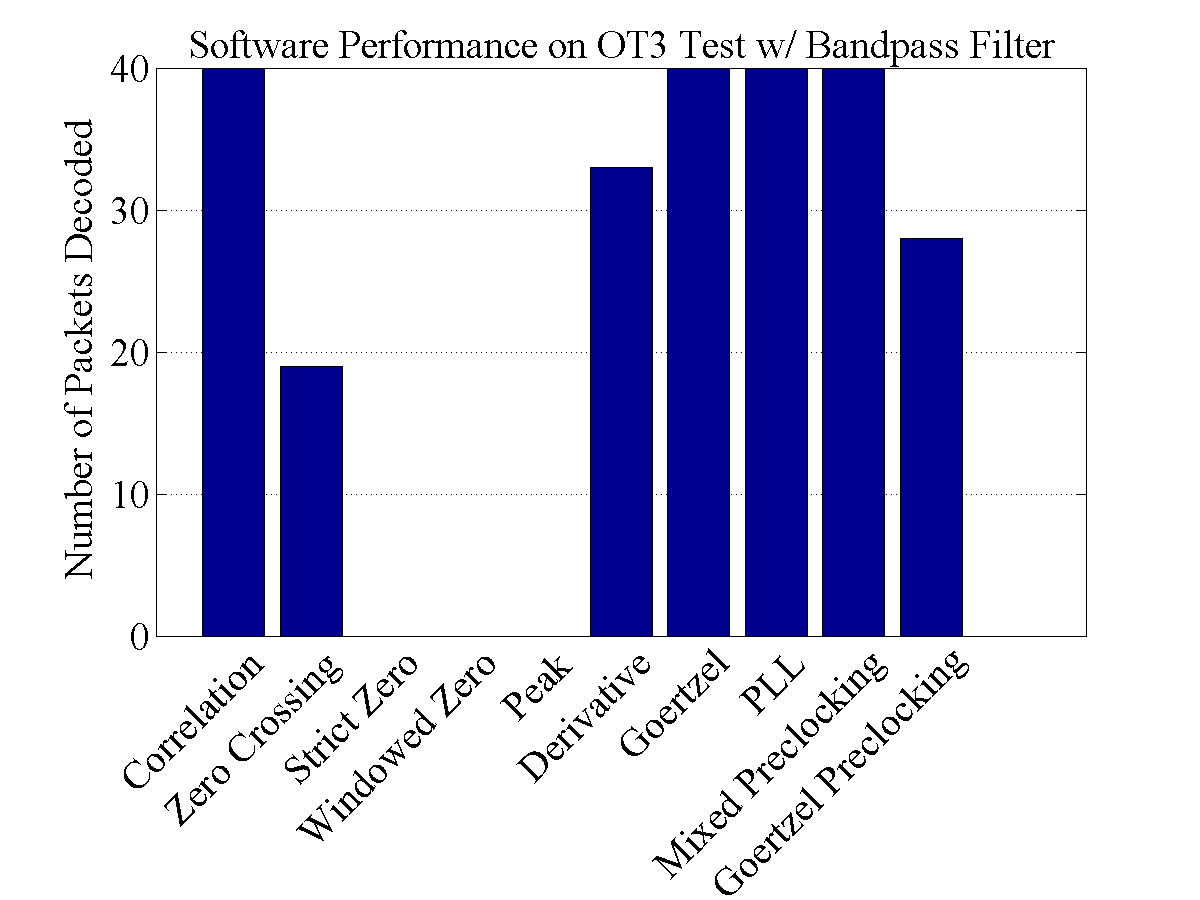
\includegraphics[width=0.75\linewidth]{images/SoftwarePerformanceonOT3TestwBandpassFilter.png} 
	\caption{Performance of software on OpenTracker 3 Test with a bandpass filter.}
   \label{OT3Filt0}
\end{figure}
\begin{figure}
  \centering
	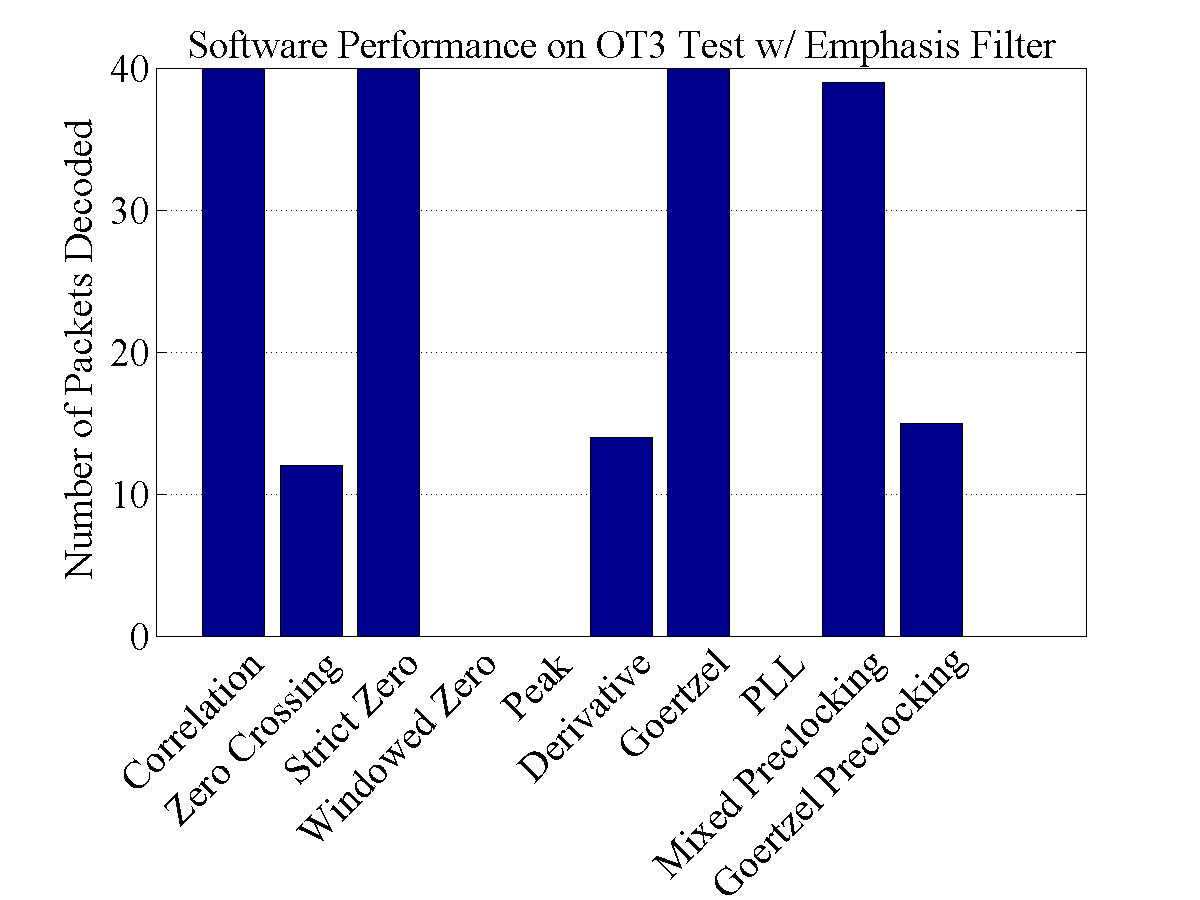
\includegraphics[width=0.75\linewidth]{images/SoftwarePerformanceonOT3TestwEmphasisFilter.png} 
	\caption{Performance of software on OpenTracker 3 Test with an emphasis filter.}
   \label{OT3Filt6}
\end{figure}
\begin{figure}
  \centering
	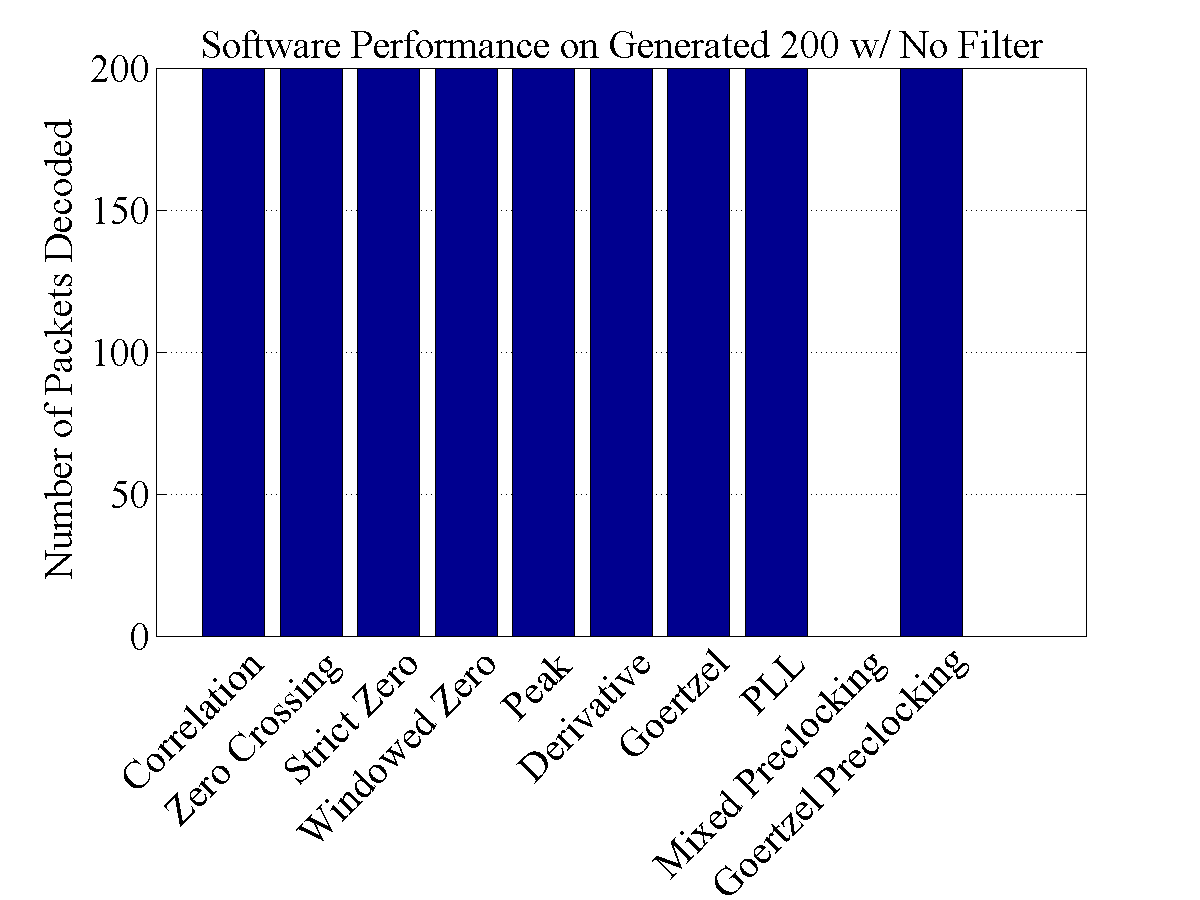
\includegraphics[width=0.75\linewidth]{images/SoftwarePerformanceonGenerated200wNoFilter.png} 
	\caption{Performance of Software on the raw signal from Generated 200.}
   \label{Gen200FiltNo}
\end{figure}
\begin{figure}
  \centering
	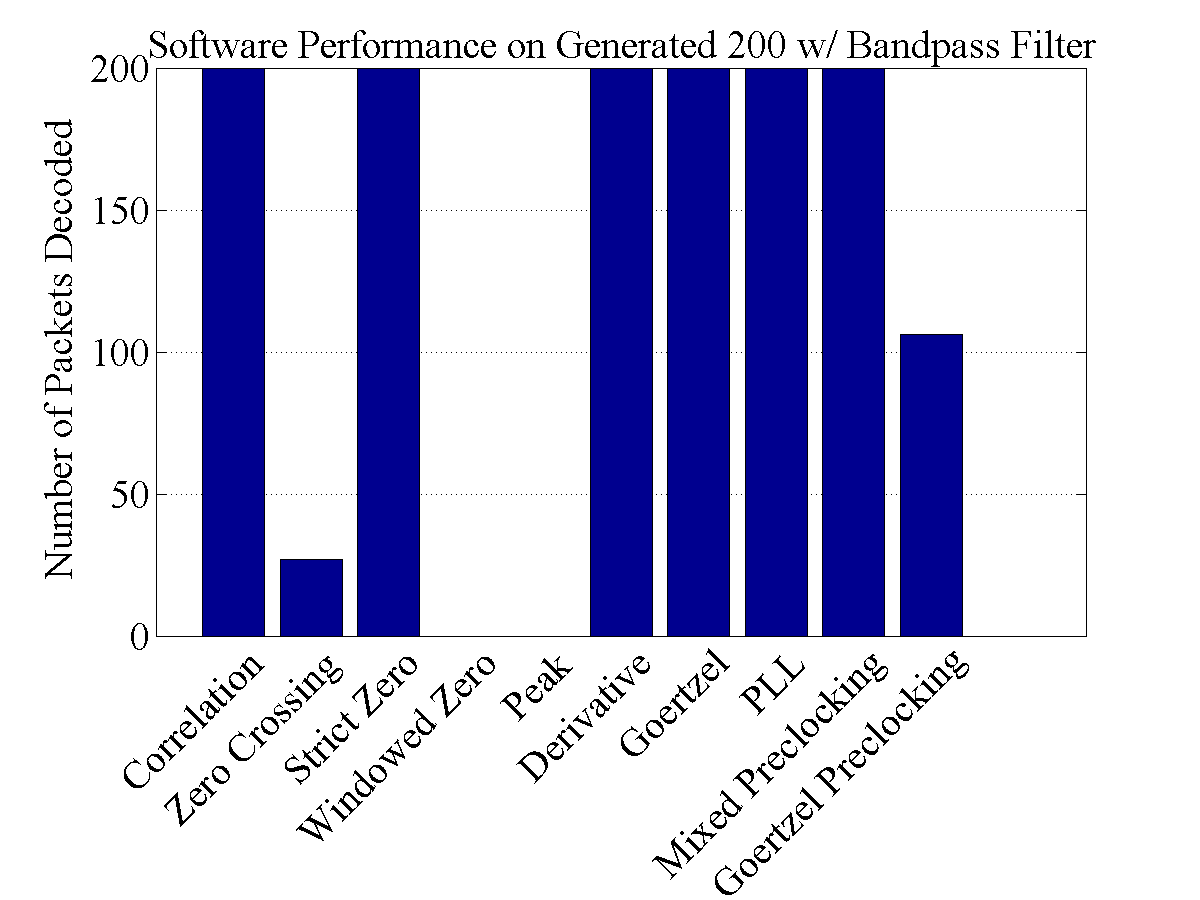
\includegraphics[width=0.75\linewidth]{images/SoftwarePerformanceonGenerated200wBandpassFilter.png} 
	\caption{Performance of software on Generated 200 with a bandpass filter.}
   \label{Gen200Filt0}
\end{figure}
\begin{figure}
  \centering
	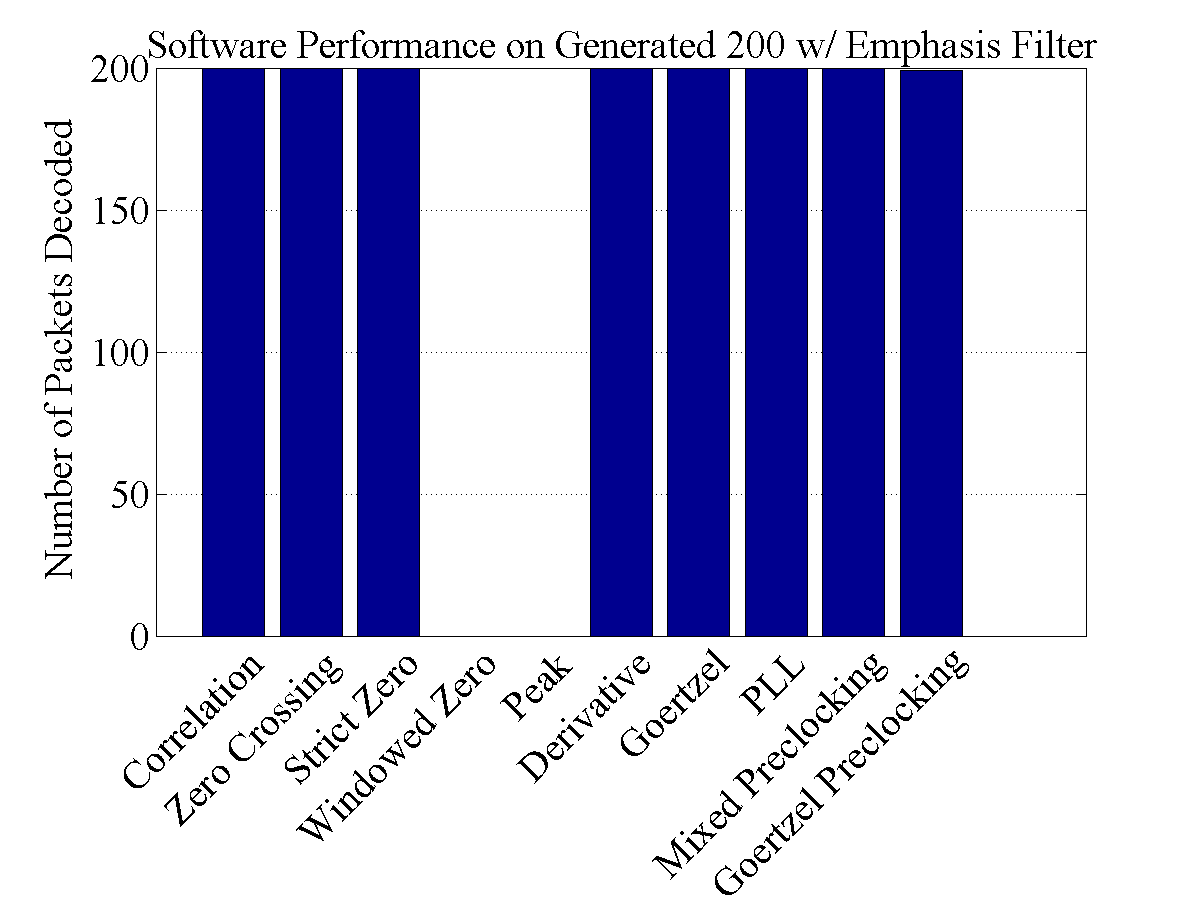
\includegraphics[width=0.75\linewidth]{images/SoftwarePerformanceonGenerated200wEmphasisFilter.png} 
	\caption{Performance of Software on Generated 200 with an emphasis filter.}
   \label{Gen200Filt6}
\end{figure}

Again, moving on from the "easy" files the performance of the software demodulators on the OpenTracker 3 Test with the noise added can be seen. Figure \ref{OTNoiseFiltNo} shows the data for the unfiltered file, Figure \ref{OTNoiseFilt0} shows bandpass filter data, and Figure \ref{OTNoiseFilt6} shows data from the emphasis filter. Two algorithms really start to shine as being comparable, and in some cases better, than the correlation demodulator. Those are the Goertzel Filter Demodulator and the PLL Demodulator. Although this is not data that was actually transmitted or received, these two start so who promise. Even the Strict Zero crossing can be seen doing well once the audio file is emphasized, but it doesn't stand up to the competition in the next two test files.

\begin{figure}
  \centering
	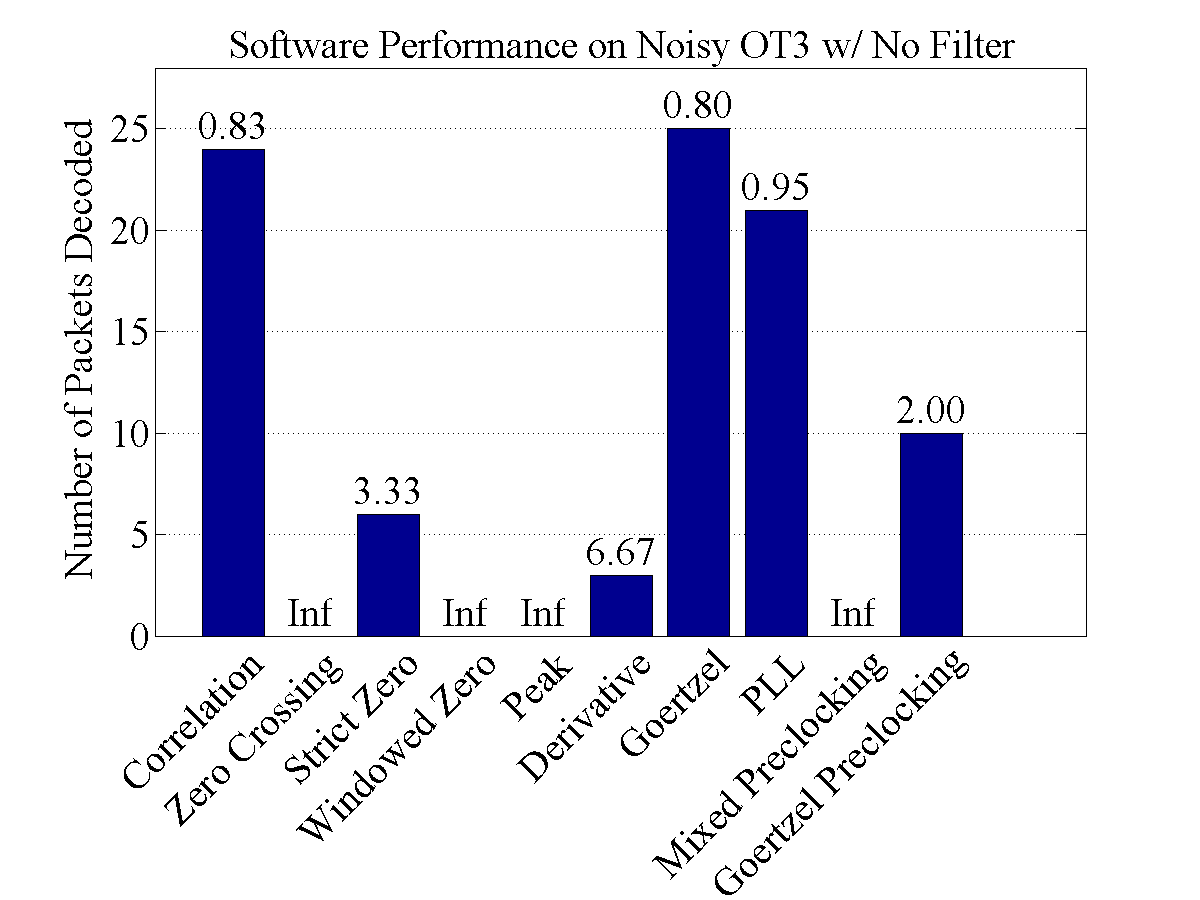
\includegraphics[width=0.75\linewidth]{images/SoftwarePerformanceonNoisyOT3wNoFilter.png} 
	\caption{Performance of software on the raw signal from OpenTracker Test with noise added.}
   \label{OTNoiseFiltNo}
\end{figure}
\begin{figure}
  \centering
	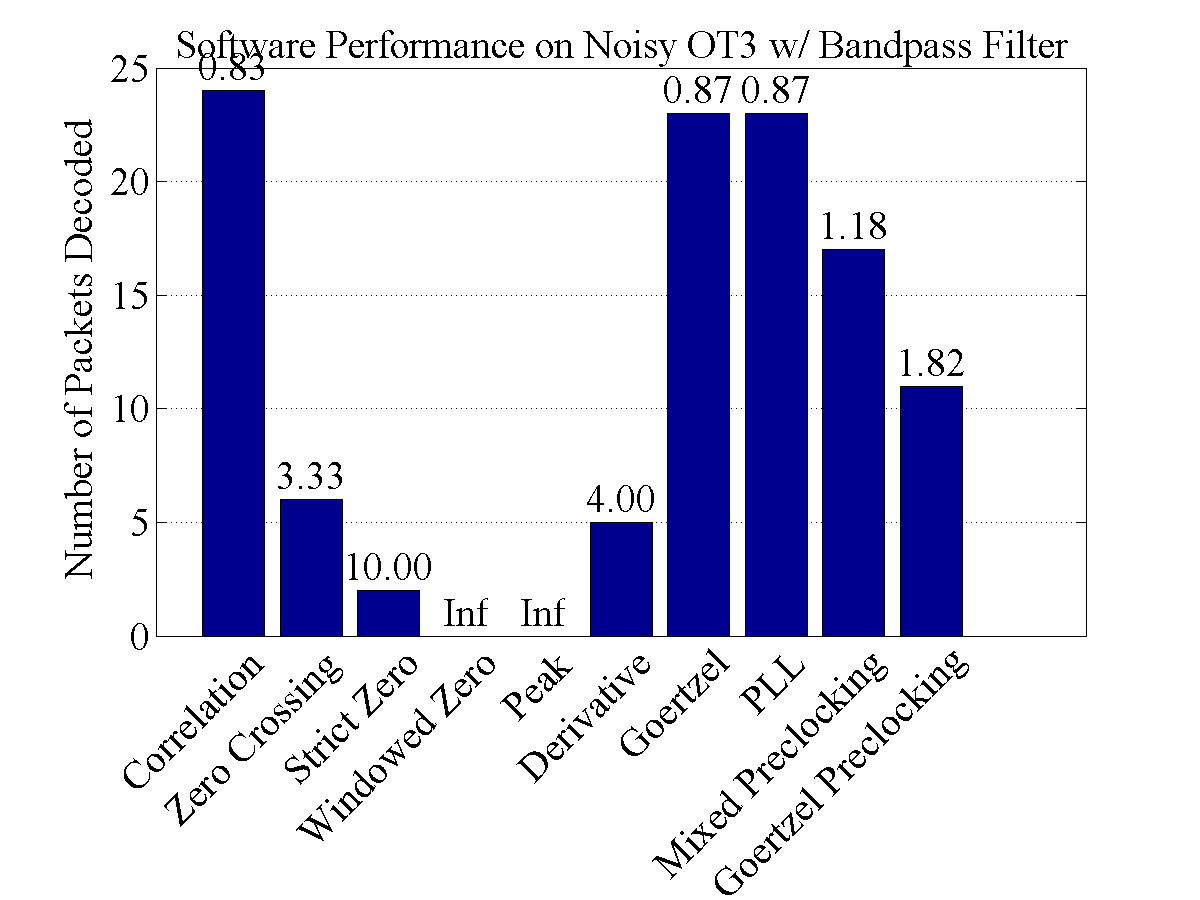
\includegraphics[width=0.75\linewidth]{images/SoftwarePerformanceonNoisyOT3wBandpassFilter.png} 
	\caption{Performance of software on OpenTracker Test with noise added with a bandpass filter.}
   \label{OTNoiseFilt0}
\end{figure}
\begin{figure}
  \centering
	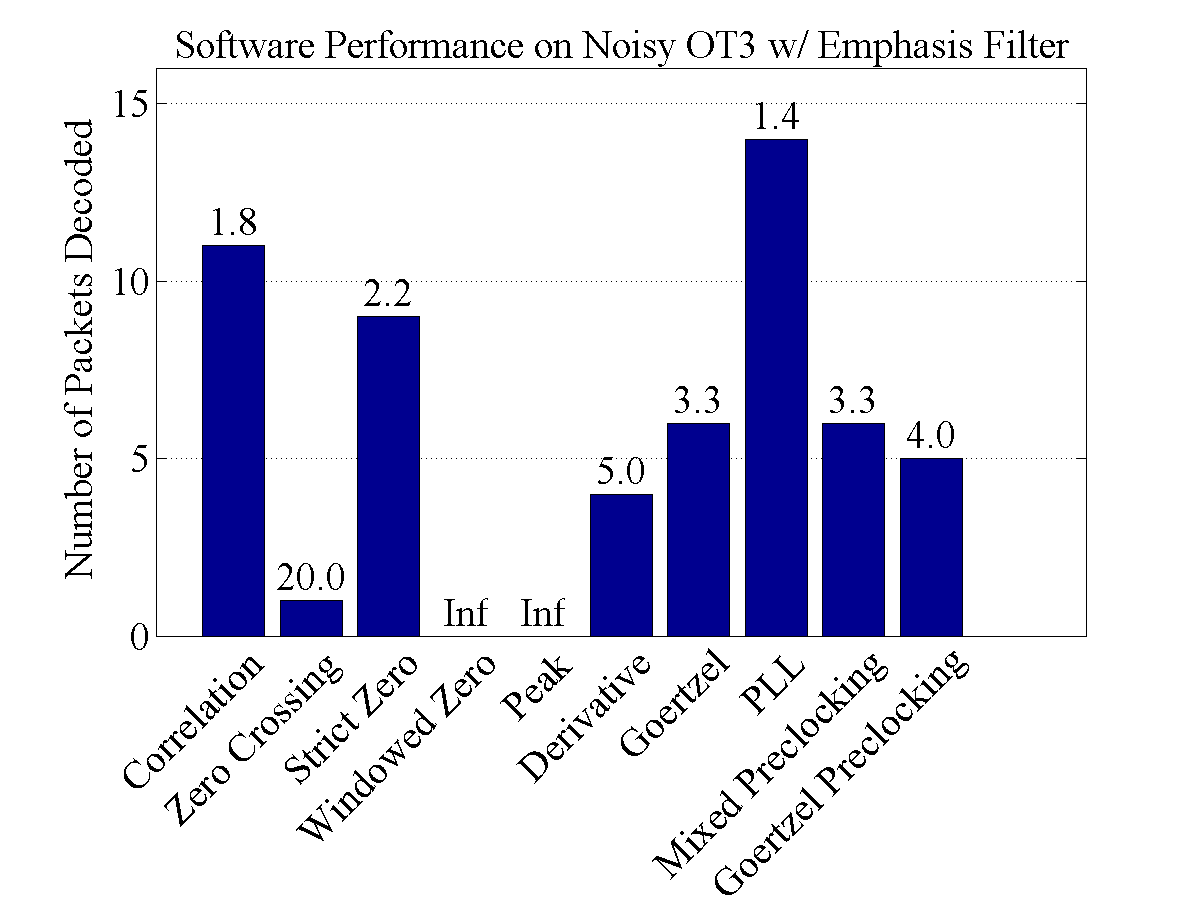
\includegraphics[width=0.75\linewidth]{images/SoftwarePerformanceonNoisyOT3wEmphasisFilter.png} 
	\caption{Performance of Software on OpenTracker Test with noise added with an emphasis filter.}
   \label{OTNoiseFilt6}
\end{figure}

As mentioned earlier, these next two test files were those that were thought the be most important to succeed at. As such, Track 1 was used to tune the algorithms since this would represent the closest real-world simulation possible. The Track 2 results are also presented for comparison. However in Track 2, in addition to being deemphasized the process of this filtering also reduced the magnitude of the signal in the audio file. As such, this file shows two things: One, the ability to pick up lower level signal and second, the algorithms tolerance to signals that were not emphasized when transmitted, but were deemphasized when received. The results of no filtering, bandpass filtering, and emphasis filtering can be seen in their respective Figure \ref{T1FiltNo}, \ref{T1Filt0}, and \ref{T1Filt6} for Track 1. The data from demodulating Track 2 can be seen in Figure \ref{T2FiltNo}, \ref{T2Filt0}, and \ref{T2Filt6}. As was caught during the OpenTracker 3 Test with noise it can be noticed that the Goertzel and PLL algorithms are still doing well on Track 1, and also the Mixed preclocking is doing fairly well. With the filter that is applied on Track 1 to create Track 2 it is basically the opposite effect of Toledo's emphasis filter and hence they cancel each other out. This can be seen by looking at the performance of the Goertzel Demodulator which does poorly with both other filterings on Track 2. However, its ability to detect low level signals and this reversal of the emphasis filtering applied makes it end of having comperable results to the just band pass filter on Track 1 - 956 versus 965. 

\begin{figure}
  \centering
	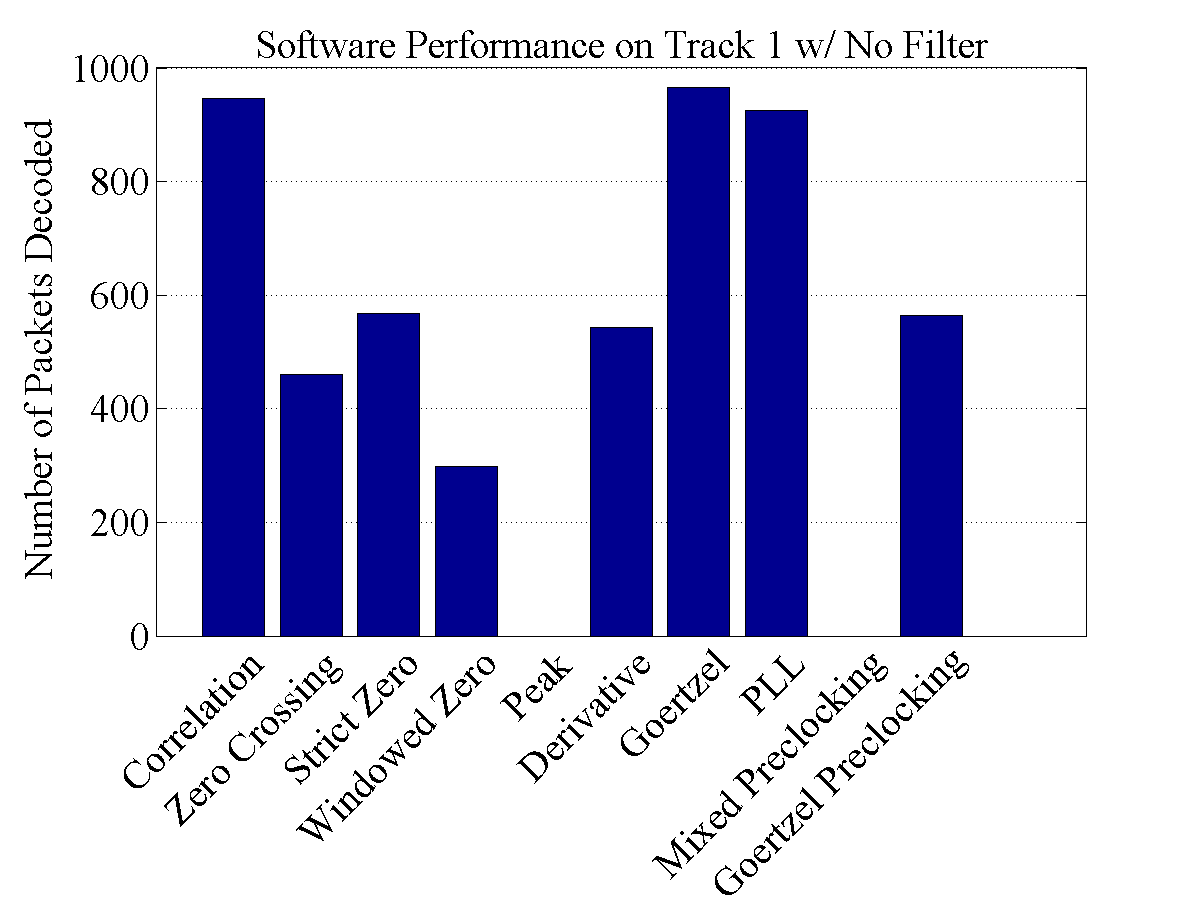
\includegraphics[width=0.75\linewidth]{images/SoftwarePerformanceonTrack1wNoFilter.png} 
	\caption{Performance of software on the raw signal from Track 1.}
   \label{T1FiltNo}
\end{figure}
\begin{figure}
  \centering
	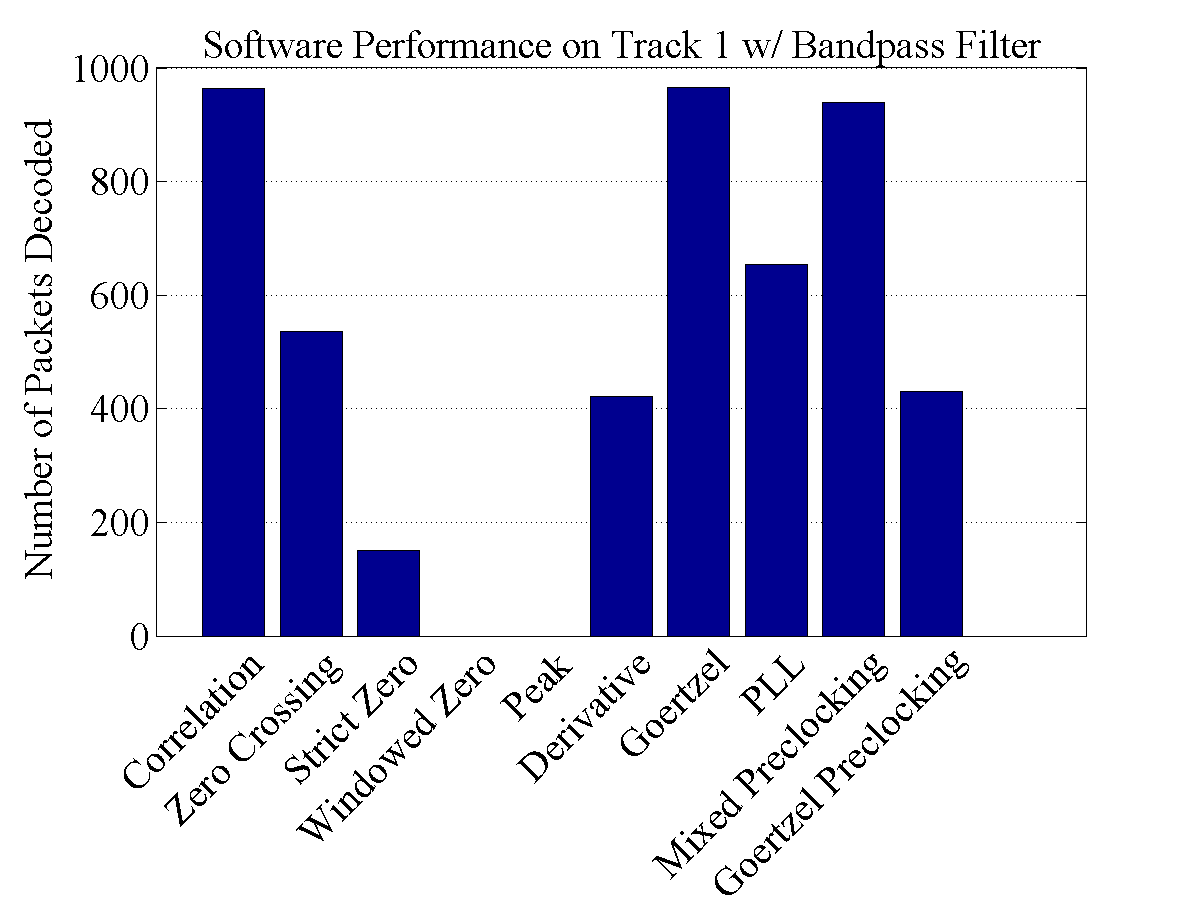
\includegraphics[width=0.75\linewidth]{images/SoftwarePerformanceonTrack1wBandpassFilter.png} 
	\caption{Performance of software on Track 1 with a bandpass filter.}
   \label{T1Filt0}
\end{figure}
\begin{figure}
  \centering
	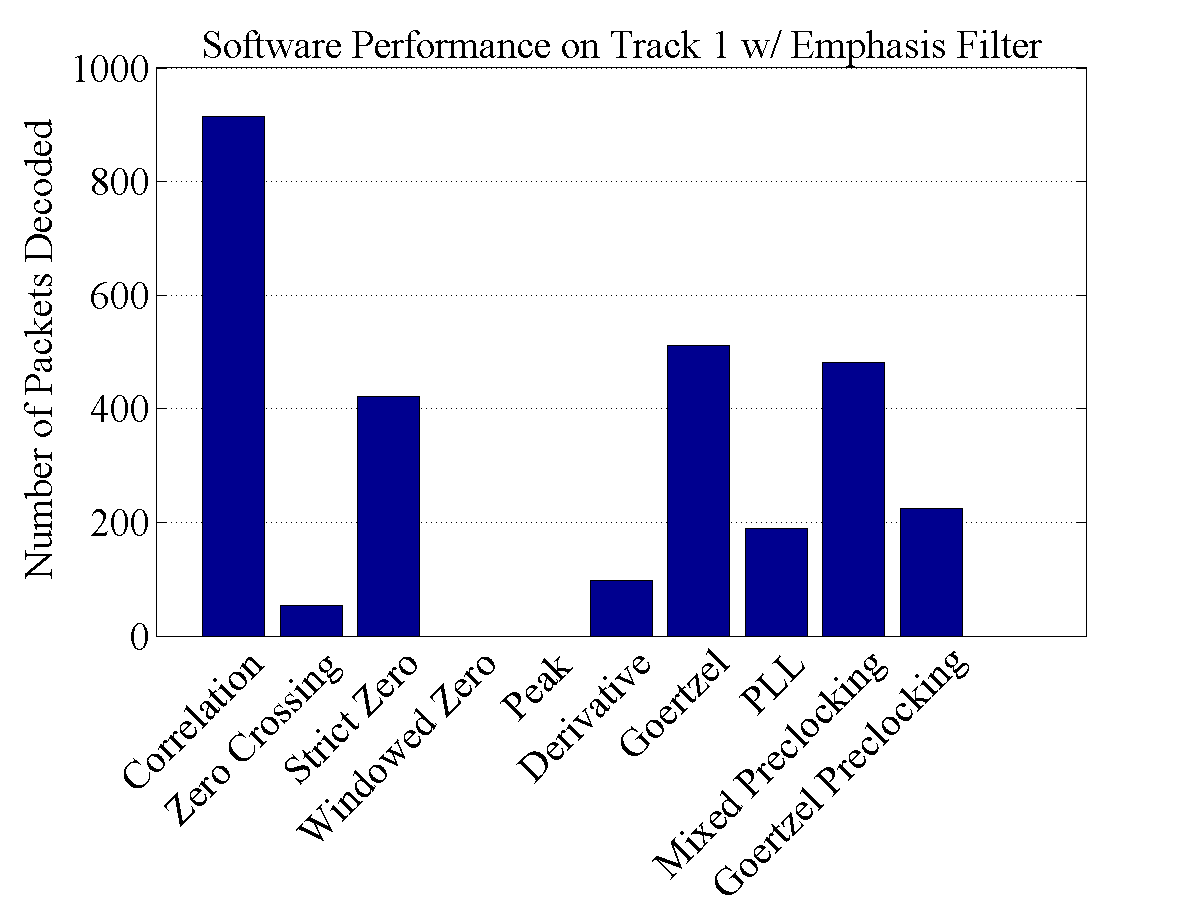
\includegraphics[width=0.75\linewidth]{images/SoftwarePerformanceonTrack1wEmphasisFilter.png} 
	\caption{Performance of software on Track 1 with an emphasis filter.}
   \label{T1Filt6}
\end{figure}
\begin{figure}
  \centering
	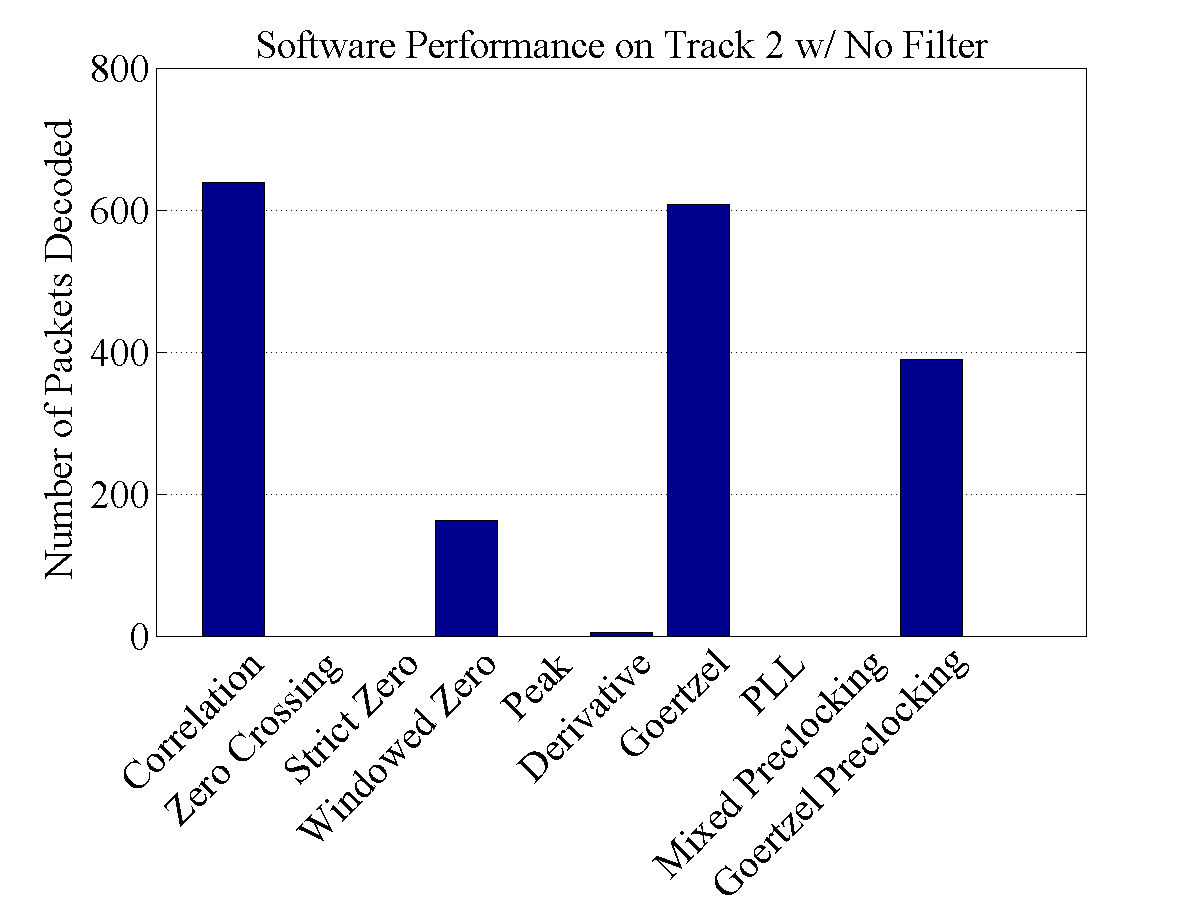
\includegraphics[width=0.75\linewidth]{images/SoftwarePerformanceonTrack2wNoFilter.png} 
	\caption{Performance of software on the raw signal from Track 2.}
   \label{T2FiltNo}
\end{figure}
\begin{figure}
  \centering
	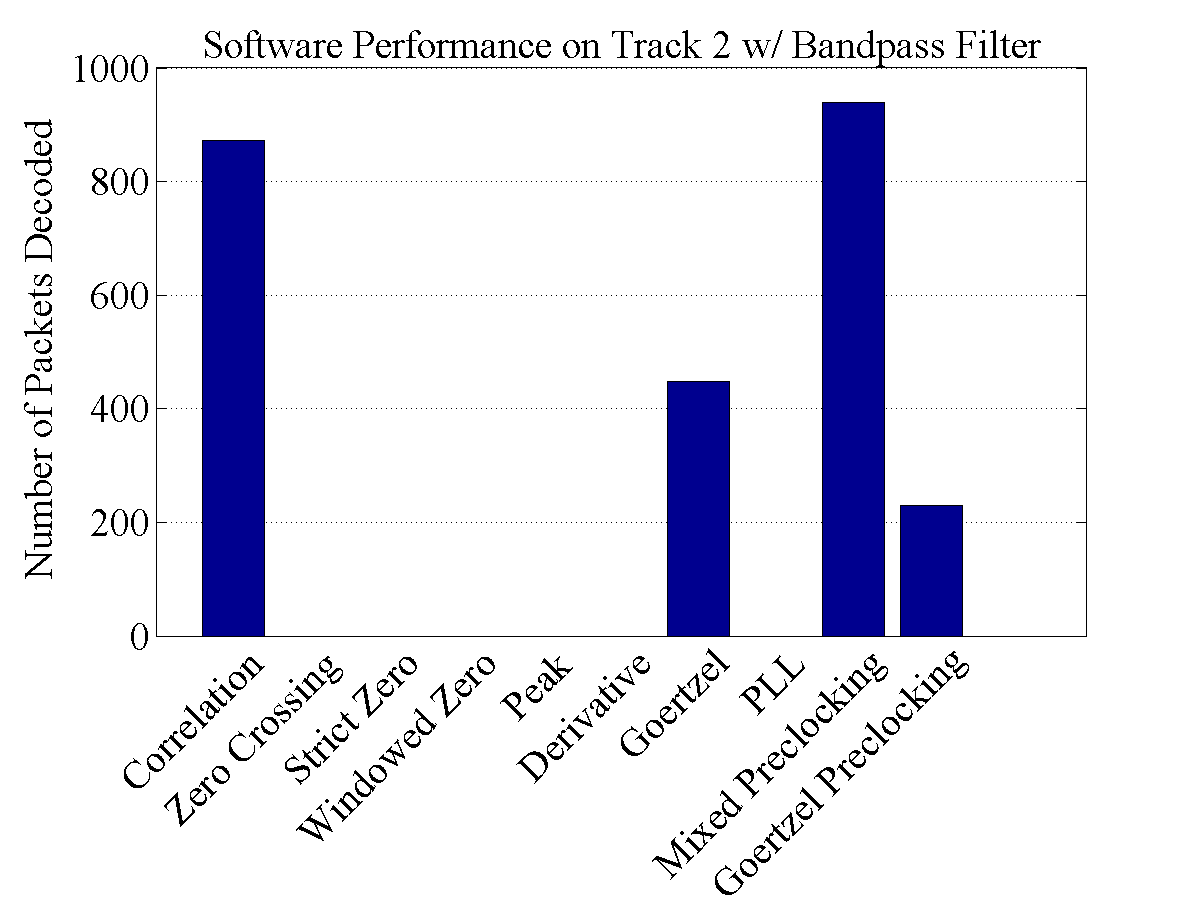
\includegraphics[width=0.75\linewidth]{images/SoftwarePerformanceonTrack2wBandpassFilter.png} 
	\caption{Performance of software on Track 2 with a bandpass filter.}
   \label{T2Filt0}
\end{figure}
\begin{figure}
  \centering
	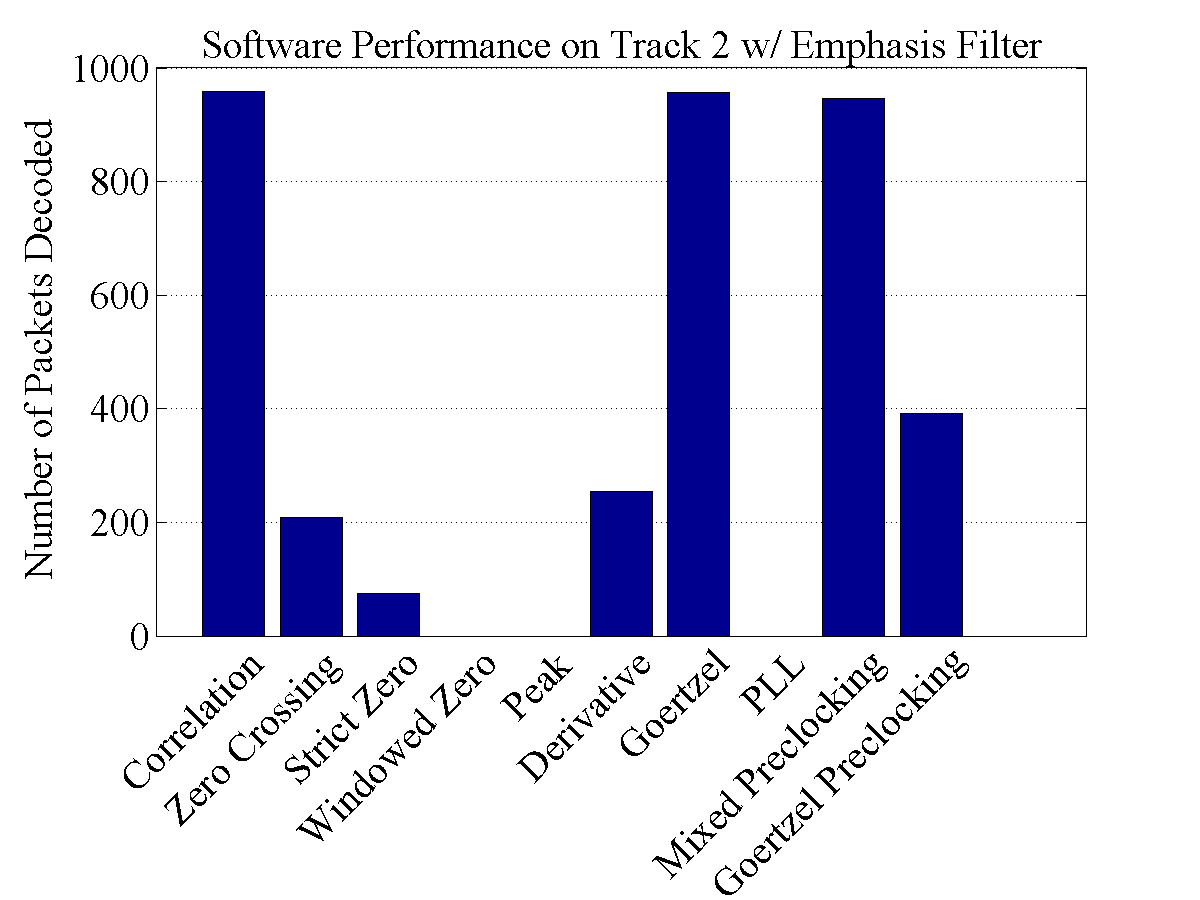
\includegraphics[width=0.75\linewidth]{images/SoftwarePerformanceonTrack2wEmphasisFilter.png} 
	\caption{Performance of software on Track 2 with an emphasis filter.}
   \label{T2Filt6}
\end{figure}


\subsection{Hardware and Software Comparisons}
It is now time to actually compare the new software implementations to the old ones as well as to the hardware. The first thing to notice is that the Goertzel Filter did very well, and in some cases better than the original correlation. Secondly, the complicated preclocking algorithm was also able to hold its own and still be a top contender. In fact the top three software algorithms were Correlation, Goertzel, and Mixed Preclocking with 964, 965, and 939 packets decoded from Track 1 with the bandpass filter. Even though they all have different number of packets decoded they each still have their expertise with being able to exclusively decode packets that others could not. For instance when the three are run together there is a total of 975 packets decoded due to the fact that Goertzel gets 12 packets that the other two do not, Correlation gets 7 that the others do not, and Preclocking decoded 3 that these other two missed. This could still be a good argument for the use of hardware over software since it is very easy to run multiple demodulators in parallel. Especially since the cost of this is only 5 minutes and 2 seconds on a file that is 25:49 long.

The question is, is the software better than the hardware? Looking at the highest numbers, no, but looking at the bigger picture, maybe. One thing about the hardware is that it is prone to variations and in need of periodic tuning. So, if instead of looking at the best of the breed, the average values are compared under the presumption that this would correspond to the average ham's decoding capabilities, then the software does decode more packets. Additionally, the software does not have any capacitors that will dry up or solder joints that may become brittle and affect the performance. The performance of the software today will be exactly the same in 5, 10, many years. The average number of packets decoded by the hardware on Track 1 was 935. Looking at this value any one of the three algorithms that are the top performers would be considered better.

\chapter{Future Work}
The sections in this chapter will explain some aspects that this project uncovered that have the potential for future research. There are three main items that I think should be explored in more depth as future work in this area of AX.25 software based demodulation, they are the discrete Short-Time Fourier Transform, the use of the checksum for forward error correction, and to actually integrate these demodulators with live traffic from a radio.

\section{The Discrete Short-Time Fourier Transform}
In a paper by Zhonghui-Chen et. al. methods are outlined to use the discrete short-time Fourier transform (DSTFT) to demodulate a binary frequency shift keyed (BFSK) signal. After a discussion of the DSTFT they go into their specific implementation, but this appears to show promise because of there results section. Granted this was for a simulation buy they showed that the error rate was lower using the DFTFT than traditional coherent demodulation even for lower signal to noise ratios \cite{Chen2008}

\section{Use the CRC for FEC}
Each AX.25 packet contains a checksum that is generated by using a cyclic redundancy check (CRC). This is used by all demodulators in order to determine if the packet that the demodulator thinks it decoded was actually a legitimate packet or just noise that happened to look like a packet. Although the CRC was not intended for forward error correction (FEC), it would be interesting to see the effects of using it as such. With algorithms such as the Goertzel algorithm the power of each symbol is determined and this power could be used to assign a level of confidence on that demodulated bit. If a packet fails the CRC check, but all except for one of the bits has a confidence greater than 80 percent, would the CRC pass if that one bit was flipped to the other symbol? This is a very good argument for the use of software since this meta data about the decoding of the packets can be kept in memory, something that most hardware is very light on. 

\section{Integrations with a Radio}
Finally another area for future work would be to integrate the new algorithms with a radio and use them to decode live data. Although the data used in the testing was a recording of live data, it would be very gratifying to be able to see these algorithms decode audio straight from the radio. Inside of javaAX25 the packages should already support it, so it should be a matter of just setting it up and letting it run. This analysis would allow for verification of the implementations functionalities as well as to be able to see how the different algorithms perform side by side in real time.


\chapter{Conclusion}
This research set out to try and prove that software could do AX.25 demodulation better than the hardware. Depending on perspective, it may have done so. However, at the very least the research shows that there are many ways to approach the challenge of demodulating these packets and presents the relative performance of over 10 software based approaches and 12 dedicated hardware approaches, whether that hardware is an OpenTracker or TNC.

In the end, the software did do better than the average result using hardware, but in the primary benchmarking file, software was only able to decode 975 packets as opposed to the 1007 that the best piece of hardware detected. Exploring some of the items in the future work section such as using the checksum for forward error correction may be able to get software to the same level as hardware, as it is close.

%\chapter{Background}

APRS is a local area awareness network designed from hams (amateur radio operators), by hams. There is a plethora of features supported within the specification of APRS including the sending of messages, bulletins, meteorological data, waypoints, objects, and most commonly GPS locations. Many of the capabilities have not been fully implemented and other implementation details are inconsistent. The goal of this research is not to discuss the shortcoming in the APRS protocol itself which lies within its implementation and use on top of the AX.25 protocol. Instead this research focuses on Layer 1 problems in the Open System Interconnection (OSI) model. 
The Layer 1 protocol for ARPS is based off of a Bell 202 modem. The Bell 202 modem was patented in 1984 using 1200Hz and 2200Hz tones, although the patent was originally filed in 1981 [1]. Interestingly, the international telecommunication union didn’t publish a standard for these modems that were used in telephone networks until 1988. In the standard, however they use 1300Hz and 2100Hz tones for symbol 1 (called a mark) and symbol 0 (called a space) respectively [2]. The basic modulation scheme is that the marks and spaces are used in a non-return to zero inverted (NRZI) encoding for the actual data. When a transition occurs from one symbol to another that symbolizes a ‘0’ bit in the original data bit stream and if the symbol remains constant over multiple symbol periods, that signifies a ‘1’ bit in the original data bit stream. It is also worth noting that there will be no more than 5 consecutive symbols during a packet, as the scheme will bit stuff in order to make sure that synchronization on the clock can be maintained. The only exception to this rule is for the flag(s) that mark the start and end of a packet. The AX.25 flag is hex 0x7E without bit stuffing. Common practice is to send multiple flags consecutively to give transmitting radio time to key up and settle and to give receiving radios time for their squelch to open.
This encoding and modulation is used to transmit the data of the APRS packets, but further background is needed in the APRS environment to discuss where this research applies. As mentioned this will not be looking into the APRS protocol itself but more focused on the Bell 202 modem and specifically the demodulation aspects. Implementing a Bell 202 modulator is simple in comparison to making a robust demodulator - especially when trying to implement one in software.

\section{Hardware Based Demodulators}

Currently there are many systems that will demodulate these Bell 202 encoded APRS packets. The original hardware used for this communication style was dedicated modems similar to dial-up 56k modems that did the encoding and decoding. These modems were connected directly to the radio and the radio would let the modem know through a signal pin if it was receiving what it thought was a data carrying signal. The terminal node controller (TNC), a modem used in AX.25 operation, would let the radio know by signaling the radio to transmit when it had data to send out. As mentioned in the introduction and early in this section, the technologies that are being used for this data transport originated in the late 1980s even though the spec for the protocol itself did not get officially released until 2000. This serves as a reminder that old hardware is commonly used that is not well understood. If a user gets something reasonable working, they will use it without doing a full analysis on edge cases or making simple modification to improve performance.
With a radio and a Terminal Node Controller, digipeaters (digital packet repeaters) are possible. Within the testing scope of this project there are two TNCs that used in order to be able to compare our results to them which were the AEA PK-88 and the Kantronics KAM Plus. Digipeaters are an essential part of the ham packet network, but many users wish to report their GPS position onto the APRS network instead of just relaying traffic for other stations. In order to accomplish this, a GPS receiver is required. Now, stations can take the data from their GPS receiver and put it in the payload of the APRS packet and transmit the GPS reported position onto the network. However, the PK-88 and the KAM Plus although used very frequently in APRS systems are not fully dedicated hardware for APRS, but instead modems that are being used for ARPS.

\section{Dedicated Hardware}

Many people know exactly what they would like to do with APRS and exactly what traffic they want to contribute to the APRS network. This has initiated dedicated hardware for APRS with a UI in order to make it simple for the end users to quickly run and configure their APRS stations. Some examples of APRS exclusive devices are ArgentData’s OpenTrackers, Byonics’ TinyTrack, and Fox Delta’s Fox Track. These compact packages along with a radio and a GPS module perform APRS tasks at a satisfactory level for many users.
Since the average user only wants to report positional information, these dedicated devices make it simple to setup. These trackers contain many features, but they don’t implement the full APRS specification. An example is the messaging service since these devices don’t have a display for the message. Certain radio manufacturers have begun to integrating the TNCs into the radios themselves to utilize the radio’s screen. The Kenwood TM-D700 series and Yaesu FTM-350 are examples.
However, both the options that were presented in section 2.1 and 2.2 require going out and buying special hardware in order to perform APRS. This can be expensive and cost prohibitive for some hams to be able to begin APRS operations.

\section{Software Based Demodulators}

It can be assumed that before a ham operator becomes interested in the APRS network and sending APRS packets that they will already have a radio. So, if they already have a radio all they have to do is buy a piece of hardware that will do the modulation in order to send a packet. However, hardware costs money and as hams are at least somewhat technology savvy most have computers. A software solution seeks to take advantage of the computer already in the operator’s possession to do the modulation and demodulation and hence offer a cheaper alternative.
This seems to be a route that some are taking and a demodulation scheme that this project explores in detail, but first some more information on current systems that operate in this software realm. Some examples of the software that can be used are George Rossopoylos’s Packet Engine or Thomas Sailer’s Linux Sound Modem. On a computer, even ones with minimal resources, there are algorithms that are being used to demodulate the APRS packets. Again, what this project aims to investigate is if improvements can be made to the algorithms used to decode these packets in order to make the software based systems more robust and as good as dedicated hardware. Preliminary testing shows that the software still has room for improvement in order to be at least as good as dedicated hardware.

%\chapter{javaAX25}

Another software based demodulator that is available is Sivan Toledo�s JavaAX25 software package. The advantage of using this package for benchmarking different algorithms is that due to his code structure and package hierarchy it makes it simple to change different demodulation algorithms. The software is hosted on github making it convenient to access the repository. The next few paragraphs will give an overview of the features that Toledo�s software package has available in it \cite{Toledo2012,javax25github}.

JavaAX25 is a comprehensive package for doing software based modulation and demodulation of APRS packets. It includes packages for interfacing with radios, sound cards, and other standard packet programs that are used on computers; one such example is that there is a plugin to be able to use JavaAX25 with AGW Packet Engine. In addition to having all of the items that are needed to be able to do the AX.25 modulation, demodulation, and interfacing with hardware, there is also a testing framework.

From within the testing framework each aspect of the software suite can be tested. The three portions that were used most extensively in this research were the modulator, demodulator, and testing framework. In order to have a demodulator one needs to have it be a child of an abstract class that implements methods for adding individual samples to the algorithms for processing, checking to see if the current signal might be a data carrier, etc. Due to the fact that the data flow was very clear for the demodulators it made it simple for different demodulators to be implemented and then tested using the �Test� class.

The main method that is called by the class using the demodulator in order to pass the data to the algorithm is the addSamplePrivate method. This method is a way for the calling class to give data to the algorithm to be processed. Each sample is a value that corresponds to the magnitude of the audio signal at that instant in time. The samples themselves derive from the fact that digital audio is sampled at a given sample rate. For this research sample rates of both 44100 and 48000 were used, but 48000 samples per second was standardized on since it divides evenly into 40 samples per baud on a 1200bps digital encoding. The goal of demodulators it to determine when a symbol transition has occurred, once this has been determined, the time elapsed since the previous transition is used to determine how many symbols have occurred. Since consecutive symbols represent a 1 bit, the number of symbols minus one will be the number of 1 bits to add to the packet followed by a zero.

The algorithm that Toledo is currently using for the demodulation is correlation based. This is done by correlating the input signal with both a 1200Hz and a 2200Hz sine wave and seeing which of the two the input signal correlates with more. Once the correlation with each is established he filters the correlation data in order to smooth the results and make it easier to be able to pull the correct frequency out of the calculations. However, before doing any of the correlation calculations the data is passed through a band pass filter centered about 1700Hz which can be seen in Figure 2.

%\chapter{Implementation}

The implementation started with a naive approach that allowed for more insight to be gained into the JavaAX25 software package. Some of the results and features that were found have been presented in the previous section. The first algorithm implemented was a Modified Zero Crossing Algorithm explained in section 4.1. Section 4.2 discusses our strict zero crossing. Section 4.3 discusses the windowed zero crossing. Section 4.4 discusses the peak detection algorithm. Our final implementation is a Preclocking demodulation algorithm and is discussed in section 4.5.

\section{Modified Zero Crossing}

As the first implementation there were some assumptions that were made that worked as a disadvantage to the demodulation. The thought behind this algorithm was to set a threshold around zero and when the value rises above this threshold centered on zero or falls below, determine that a zero crossing occurred. The time between subsequent zero crossings can be calculated in terms of the number of samples and the sample rate of the incoming audio can be used to figure out the time between the zero crossings in seconds.

One can calculate the time between zero crossings by realizing that they happen every p radians or twice in one frequency period. The period T can be calculated using T = 1 / f where f is the frequency. Using this information and the knowledge that the two tones are 1200Hz and 2200Hz one should expect zero crossings every 833�s and 455�s respectively. This logic of extrapolating the frequency from the zero crossing spacing of the signal is used for this as well as the next two algorithms presented in sections 4.2 and 4.3.

Upon implementing this algorithm there was an apparent disadvantage to using the threshold around zero. The original thought with this threshold is that it would help to get rid of erroneous zero crossings caused when there was low level noise on the signal. However, this buffer was not at all helpful since it doubled our opportunity for error on a zero crossing. If there was noise on the signal both right before entering the threshold and right before exiting this threshold it allowed for two separate contributions to error on figuring out exactly what sample number the crossing was at. Noticing this flaw the next algorithm, called the strict zero crossing, is exactly as the name implies; a strict zero crossing demodulation algorithm instead of having a threshold around zero.

\section{Strict Zero Crossing}

The strict zero crossing algorithm had advantages over the initial zero crossing algorithm implemented since it only has one area where error can occur. Unlike the algorithm in section 4.1 the zero crossing corresponds to exactly one value sample as opposed to relying on two samples in order to the back calculate the zero crossing.

The initial algorithm kept track of whether the signal was high (above zero) or low (below zero) and then when it transitioned to the opposite this was considered a zero crossing. The spacing between crossings was then used to calculate what frequency must be present in the signal using the logic explained in section 4.1. The initial results for this algorithm were good with clean signals, but once any noise was introduced, it still suffered from the same problems as the first Zero Crossing algorithm which was that the noise was bumping the zero crossing values around.

One example of the zero crossing weakness to noise was having 1200Hz tones that looked like 2200Hz tones. This case arose when the noise made one of the 1200Hz crossings happen a little late and then the subsequent zero crossing for the 1200Hz crossing a little early. This now smaller time between what should be a 1200Hz crossing distance now instead looks like a 2200Hz tone. In order to alleviate some of the trouble caused by this random white noise some filtering was added. See Figure 3 for an example of noise corruption.

At first the filtering chosen was just an average of the two adjacent points. This had better results for some cases, but not for all. For instance, if the noise was just affecting one zero crossing used for the calculation of the frequency it helped, but if the noise was affecting both zero crossings that were needed to figure out the frequency then we found that moving up to an average of three points proved to have the best results in terms of total number of packets decoded. This does makes sense though since if the noise causes the signal to jump either above or below the true value and averaging the three adjacent points allowed for two of them to be very noisy and cancel each other out while still having one to keep the filtered value from the averaging as close as possible to the original signal.

In addition to doing a straight averaging of the three adjacent points, some effort was put into doing a weighted average. The results from the weighted average were not as good since the whole point was to try and filter out some of the noise. If specific points were weighted instead of doing the unweighted average it meant that the goal of the filtering through averaging was useless. This is because if more weight is put on any one of the value it means that the noise in that point could overwhelm the calculation, and as mentioned then throw off the point of the filtering which is to get a closer approximation to the original signal value.

\section{Windowed Zero Crossing}

Although the strict zero crossing was much better than the original zero crossing algorithm there were still improvements that needed to be made. The filtering that was done through averaging adjacent points helped, but in some extreme cases it was still not enough. The next algorithm relied on averaging the averages. Basically instead of just looking on a crossing to crossing basis, a sliding window about the length of a symbol period is used, and the crossings within that window counted. The thought was that this would place less dependence on each zero crossing being calculated correctly since it is only one data point and hopefully the other one or two in the window will make correctly determining the frequency of the tone present in the signal more accurate. 

In order to make it more deterministic how many crossings were expected in the window a window size slightly less than one baud was chosen. The reason for this is that for a 1200Hz tone if the size of the window is just one sample greater than a symbol period there may be 3 crossings in the window since the signal is 1200 bps and hence the 1200Hz tone can complete one full period during the time elapsed in one symbol period. Making the window slightly less, 90% the size, than the symbol period ensures that noise will not interfere with the crossing count and that within the window there will only ever be 2 crossings if a 1200Hz tone is present in the window. If there are less than two crossings in the window then there is just noise / a DC offset and greater than 2 crossings is assumed to be a 2200Hz tone. This may seem like a far leap, what if there is noise at 20,000Hz? This was handled by requiring a minimum time to elapse between crossings that was a little less than that expected for subsequent 2200Hz crossings. This does mean that the algorithm will favor 2200Hz tones over 1200Hz tones when in the noise, but it still picks up the 1200Hz tones fairly well.

This theory and approach is all fine and dandy up until actually applied. Although, it originally seemed like a good idea, there were problems with setting all the values �correctly.� For instance there are three apparent variables that can be tweaked in order to change the performance: 1. the size of the window, 2. how many crossings should be expected within the selected window size, and 3. the amount of time to wait before allowing a zero crossing the be considered a zero crossing. Modifying these three parameters showed many different results in terms of the total number of packets decoded by the algorithm. For instance in the Open Tracker 3 test file that had 40 packets in it (more information on it in section 5) the algorithm could decode 39 of the packets with the window size set to 90% of a symbol length and the number of successfully decoded packets would drop if the window size was decreased below 87% or increased above 93%.

\section{Peak Detection}

The peak detection demodulator was developed to try and mitigate some of the problems observed with the strict zero crossing method. This takes advantage that peaks will occur on exact sample intervals while zero crossings samples don�t typically don�t occur directly at the crossing. This delay for the zero crossing can lead to ambiguity by a sample or two on either side of the zero crossing. The number of samples between the zero crossings can be either expanded or compressed by a few samples causing misidentification. By using peak detection this ambiguity could be further reduced. 

The algorithm uses the absolute value of the time domain to move the troughs to be peaks so transitions can be detect if they occurred during the peak to trough transition using the peak algorithm.  A three sample average is used for each incoming sample to help smooth the noise present. Three samples blends the noise while still preserving the integrity of the shape of the sinusoidal signal. The current sample is then compared to the previous local peak and stored if it�s higher along with the sample index number. If the two previous samples are consecutively decreasing a peak has occurred and the signal is moving in the downward direction. The handlePeakDetection() method is then called and after processing is completed the resets the local peak, local peak index, samples since the previous peak, and moved into the decreasing state. While in the decreasing state, the algorithm determines if the state has changed to increasing when three consecutive samples are larger than the previous. Once the increasing state has been entered, the algorithm repeats waiting for a peak.

The handlePeakDetection method first determines the number of samples between the current and previous peaks. This value is then subtracted from the previous number of samples between peaks. If the difference is greater than a threshold a transition has occurred. Once a transition has been detected, the number of bits is determined and the previously mentioned packet creating process in the JavaAX25 documentation is utilized.

The peak detection demodulation method was able to detect extremely clean source signals, but struggled against real world signals. It was difficult to tweak the algorithm to decode packets. Changing the difference threshold would help in some cases, while hurt in others making no perfect solution. Many packets had only a few bit errors. This approach could maybe be improved by averaging the previous peak periods to more clearly determine a transition occurrence, but due to time constraints more effort was put into the next demodulation technique. 

\section{Preclocking Demodulation}

Using the information collected thus far and the now greater knowledge of the software package as a whole the next algorithm is considerably more complicated. There are size different steps to the algorithm. First, filter the data to remove noise and higher frequency components and make the signal smoother. Second, look for flags in the signal so that the demodulation can happen one packet at a time instead of just blindly trudging forward through the packet sample by sample. Third, take the derivative of the whole packet to and determine the zero crossings. Fourth, frequency transitions are extrapolated from the derivative data. Fifth, the frequency transitions of the packet clocking are calculated and finally, sixth the tone demodulation is done on a baud by baud basis.

The original goal with this much more complicated algorithm than its predecessors was to take advantage of the clocking of the original signal. Using the clocking in the digitally encoded signal, more confidence can be instilled into making sure that every symbol gets demodulated correctly. The filtering and flag finding is done using the preexisting code that Toledo wrote, so not that many details will be included about it here. Instead the explanation of the inner working will start with why the derivative of the input signal was used. The nice thing about using the derivative in this algorithm instead of the original signal is that it solves two previously encountered problems: 1. the DC offset problem and 2. the emphasis problem. DC offset is when the oscillation of the frequency doesn�t occur around zero, but has been biased around a different DC voltage. This can occur in hardware due to the different strengths of the two signals. If a 1200 Hz tone has a higher magnitude than the 2200 Hz tone the 2200 Hz can be off centered on the voltage at the transition time. This can be observed in Figure 4. The Bell 202 signal is typically FM modulated onto a carrier for RF transmission and FM Modulation tends to attenuate higher baseband frequencies. In audio systems the higher frequencies are amplified before FM modulation and then attenuated after demodulation on the receiver. This creates a stronger 2200 Hz tone. There is no standard practice among amateur APRS users as to how/when to emphasis or de-emphasis packets. This creates the need diverse detection criteria to address the biasing of either 2200 Hz or 1200 Hz without knowing ahead of time which emphasis state has occurred. See Figures 5 and 6 for examples. Due to the nature of the derivative the DC offset problem is solved very literally, but solving emphasis problems is not necessarily as obvious, however it still shows improvements over the original signal. See Figure 7.

Once the data is filtered through both the direct FIR band pass filtering and through the derivative the frequencies seen in the packet are stored and using linear interpolation the exact point that each frequency transition occurred at is stored. Since frequency transitions will only happen along baud borders this allows for the clocking to be extrapolated from these transitions. The clocking is then determined in terms of offset in samples from the start of the possible packet. This is done through going through each one of the possible clockings (for a 48000 sample per second audio source this works out to 40 possible alignments) and selecting the sample offset number that minimizes the square distance between that perceived clocking and the observed transitions. 

Once the clocking is determined the frequency data that was calculated using the zero crossing from the derivative is used in order to figure out the actual tone that is contained within each baud. Two different approaches were tried to extrapolate the frequency out of the symbol window. First it was thought that taking the average of each one of the frequencies that fall within the baud period that just calculated would be best, but it became apparent that the filtering and derivative was not enough. Within decoding of legitimate packets frequencies greater than 5,000Hz were detected skewing the 1200Hz tones to look like 2200Hz when averaged. Another approach of just taking the one value directly in the middle of a baud period was used, but this didn�t prove to be worse. The minimum amount of time to pass between zero crossings in the algorithm was modified to try and get more accurate frequency results. Then the detected symbols were histogrammed to see how many determined frequencies were ambiguous between 1200-2200Hz. The result showed a clear division between the two frequencies and the threshold was set in the middle at 1700 Hz for the average of the frequencies inside the baud period as seen in Figure 8. The end results explained in more detail below show prove that this algorithm is on par with the original correlation algorithm and can decode some packets that it could not.

%\chapter{Testing}
In order to be able to evaluate the results from this research, each demodulation technique considered needs to be tested and the number of packets that each technique was able to successfully decode needs to be compared. From this analysis, it will be seen which techniques are effective and are able to decode relatively more packets as opposed to those that decode fewer. In order to validate the techniques results for dedicated hardware will also be collected for comparison. The testing for both the dedicated hardware and the software algorithms will be described in the corresponding sections below.

\section{Hardware Testing Setup}
The testing setup for the hardware is fairly simple since they are basically black boxes that just need to be supplied with the correct inputs. Each piece of hardware has two connections; one is the radio port, and the other is the serial connection. As the name implies, the radio port is used to be able to interface with the radio. This port has connections such as transmit audio, receive audio, push-to-talk (PTT), supply voltage (VCC), and ground. A digram of the common radio port can be see in Figure \ref{RadioPortPinout} and found in any manual including those of Argent Data\,\cite{Systems2013}. Since this was common between multiple pieces of hardware, a simple break-out board was created that allowed for a more universal audio transport mechanism of 3.5mm tip-ring-sleeve connectors, and also a 2.5mm barrel jack for power. This was much simpler than actually interfacing with a radio since the audio could just be played from a computer into the device; this device can be seen in Figure \ref{BreakOutBoard}. 

\begin{figure}
  \centering
	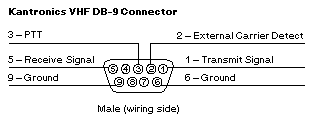
\includegraphics[width=0.75\linewidth]{images/RadioPortPinout.png} 
	\caption{Example Radio Port pin out for Kantronics, also consistent with others including OpenTrackers\,\cite{Martin2014}.}
   \label{RadioPortPinout}
\end{figure}
\begin{figure}
  \centering
	\includegraphics[width=0.75\linewidth]{images/BreakOutBoard.png} 
	\caption{Break-out board fabricated for hardware testing. There are two audio ports on the board; one for audio in and the other for audio out. On the right is the barrel jack fro supplying power.}
   \label{BreakOutBoard}
\end{figure}

\section{New javAX25 Demodulator Testing Framework}
Included within the javAX25 suite was a testing application that could both generate and decode packets. However, it was limited to only being able to specify one audio file and one demodulation algorithm. Using this test file as a basis, a new testing application was created that allowed for the multiple demodulators to be compared side by side against multiple audio files with a single run of the application. In addition to the output being printed to the console, the output was also saved to a file. Having these features in the testing application allowed for a much more streamlined analysis of all the algorithms collectively and tuning individual algorithms. One very convenient aspect of programmatically testing is that it is very easy to add a loop to try a range of tuning parameters and then look at the results to decide what is the best option. All of the results listed in the following chapter are from the testing application and mechanism described here.

%\chapter{Results}
This results chapter is meant as a mechanism to present all of the data that was collected on the performance of different demodulators. All of the demodulators that were tested in the course of this research will be shown, whether it be dedicated hardware or software. The first results that will be shown are those of the dedicated hardware, being TNCs and Argent Data's OpenTrackers. Following the hardware will be the software implementations. Following these two categories will be some general comparisons between them.

\section{Dedicated Hardware Results}
In the scope of this research a total of 12 pieces of hardware were tested. They include Argent Data's OpenTracker 2, OpenTracker 3, OpenTracker USB, OpenTracker 3 Micro, Kantronics Kam, two Kantronics Kam Plus, two AEA PK-88, a PK-232, a PK-232MBX, and an MFJ-1278. Hardware models for which more than one was tested will be differentiated by a number in parentheses following the model number. Please note that on the figures OpenTracker will be abbreviated OT.

The first two tests consisting of clean packets - 40 generated from the OpenTracker and 200 using Toledo's suite - was relatively uninteresting. Essentially every piece of hardware decoded all 40 and all 200 packets. The only anomalies to this were that the OpenTracker USB was only able to decode 39 and 193 out of the 40 and 200 packet files respectively. Additionally the OpenTracker 3 Micro missed one packet in the 200 packet file to only decode 199. Since there is no real way to debug and see the cause of decoding relatively fewer or more packets just the data for these hardware items is presented as it was measured to allow for comparison to the software. This will continue to be the case for the remainder of this hardware section.

Following the two easy files the next file is same content as the file with 40 packets in it, with the only difference being that noise was progressively added. In Figure \ref{allHardwareOT3Noise}, the two PK-88s stand out for being able to decode 25 of the 40 packets in this file.

 \begin{figure}
  \centering
	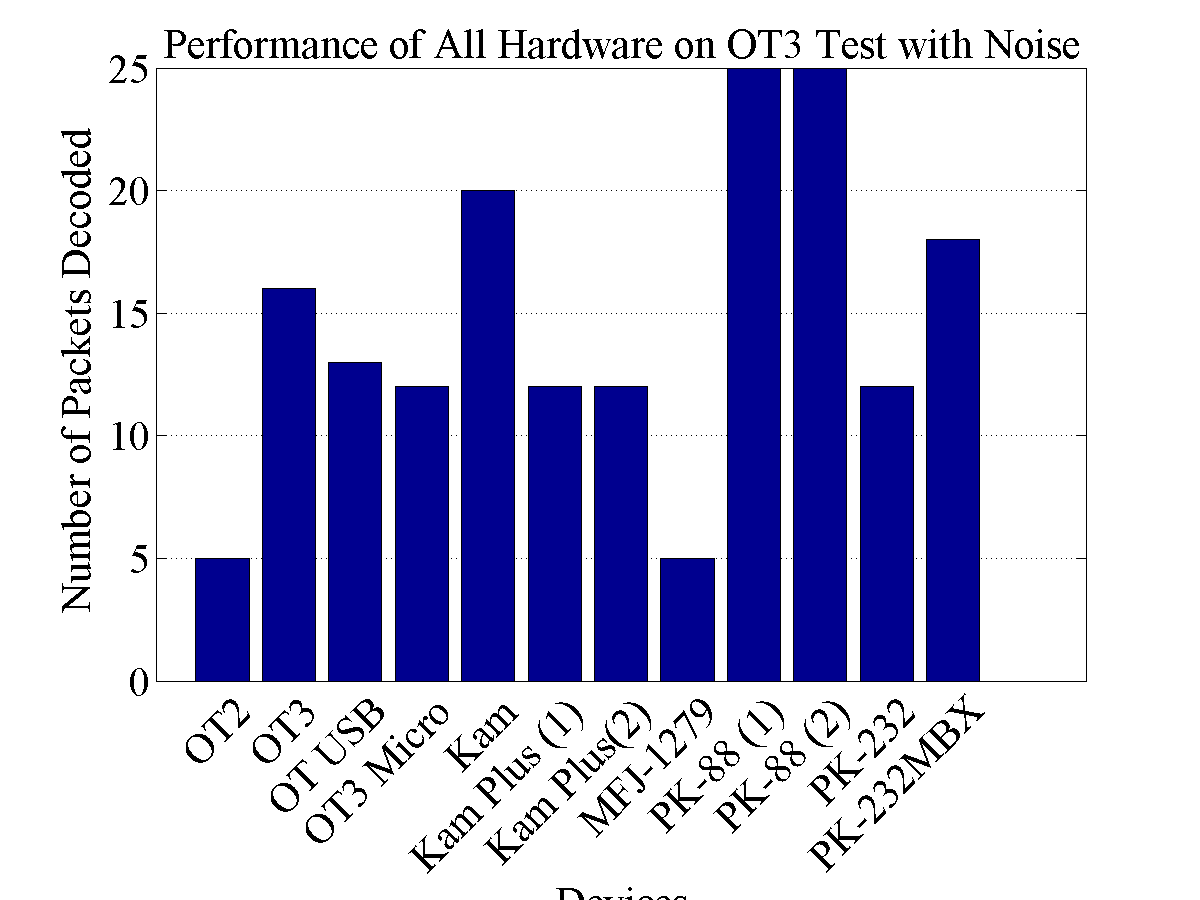
\includegraphics[width=0.75\linewidth]{images/PerformanceofAllHardwareonOT3TestwithNoise.png} 
	\caption{Number of packets successfully decoded for all tested hardware on the OpenTracker 3 test file with noise.}
   \label{allHardwareOT3Noise}
\end{figure}

The next two files are the ones that were used most extensively in the testing for comparison and tuning. Primarily the first, which is just a recording of traffic off the air. They are Track 1 and 2 from the APRS CD mentioned in the Demodulator Benchmarking Chapter. The results from Track 1 are in Figure \ref{allHardwareTrack1} and Track 2 in Figure \ref{allHardwareTrack2}. The top three performances of the hardware on Track 1 were the PK-88 (2) with 1007 packets decoded, the Kam with 988 Packets, and the Kam Plus (2) with 985 Packets. For Track 2 the top hardware was the Kam Plus (2) with 998, the Kam Plus (1) with 967, and the Kam with 938.

 \begin{figure}
  \centering
	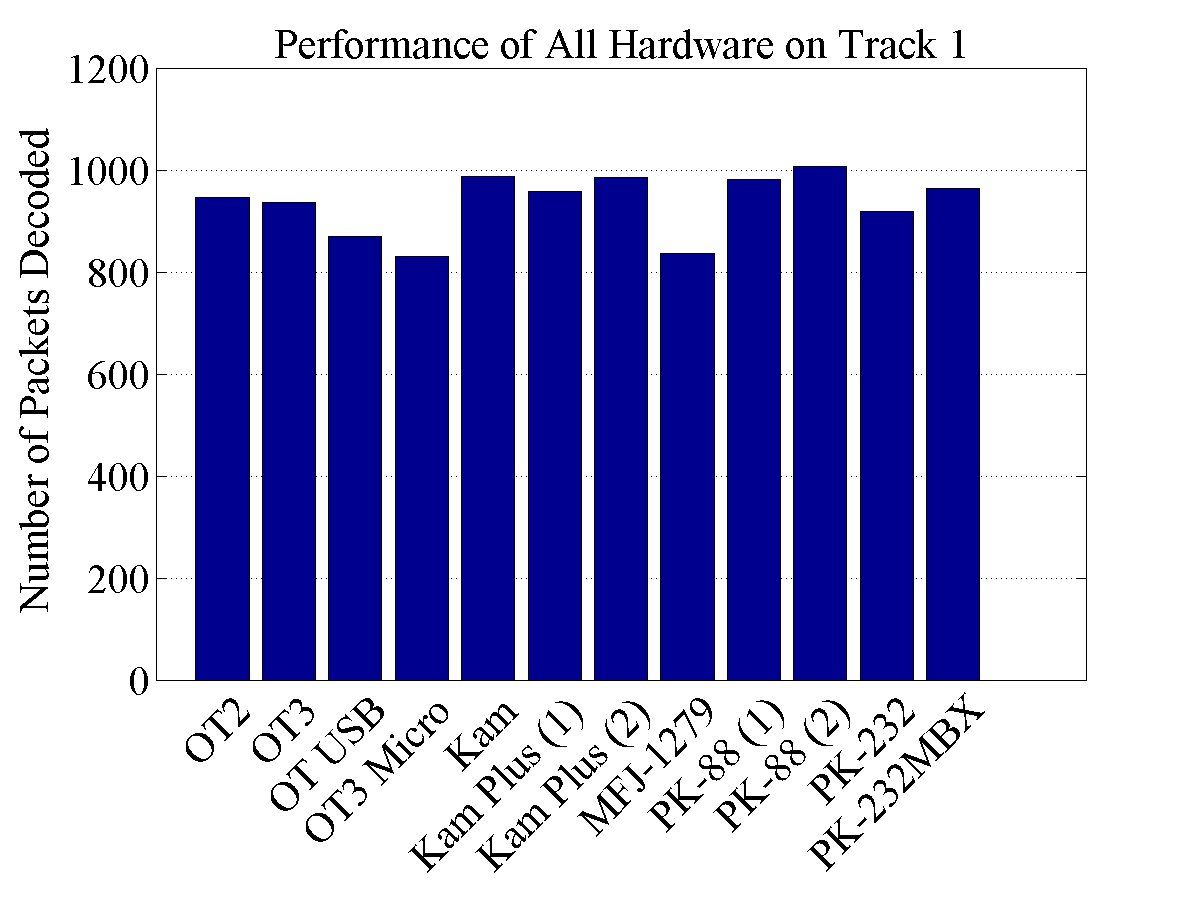
\includegraphics[width=0.75\linewidth]{images/PerformanceofAllHardwareonTrack1.png} 
	\caption{Number of packets successfully decoded for all tested hardware on the Track 1 test file.}
   \label{allHardwareTrack1}
\end{figure}

 \begin{figure}
  \centering
	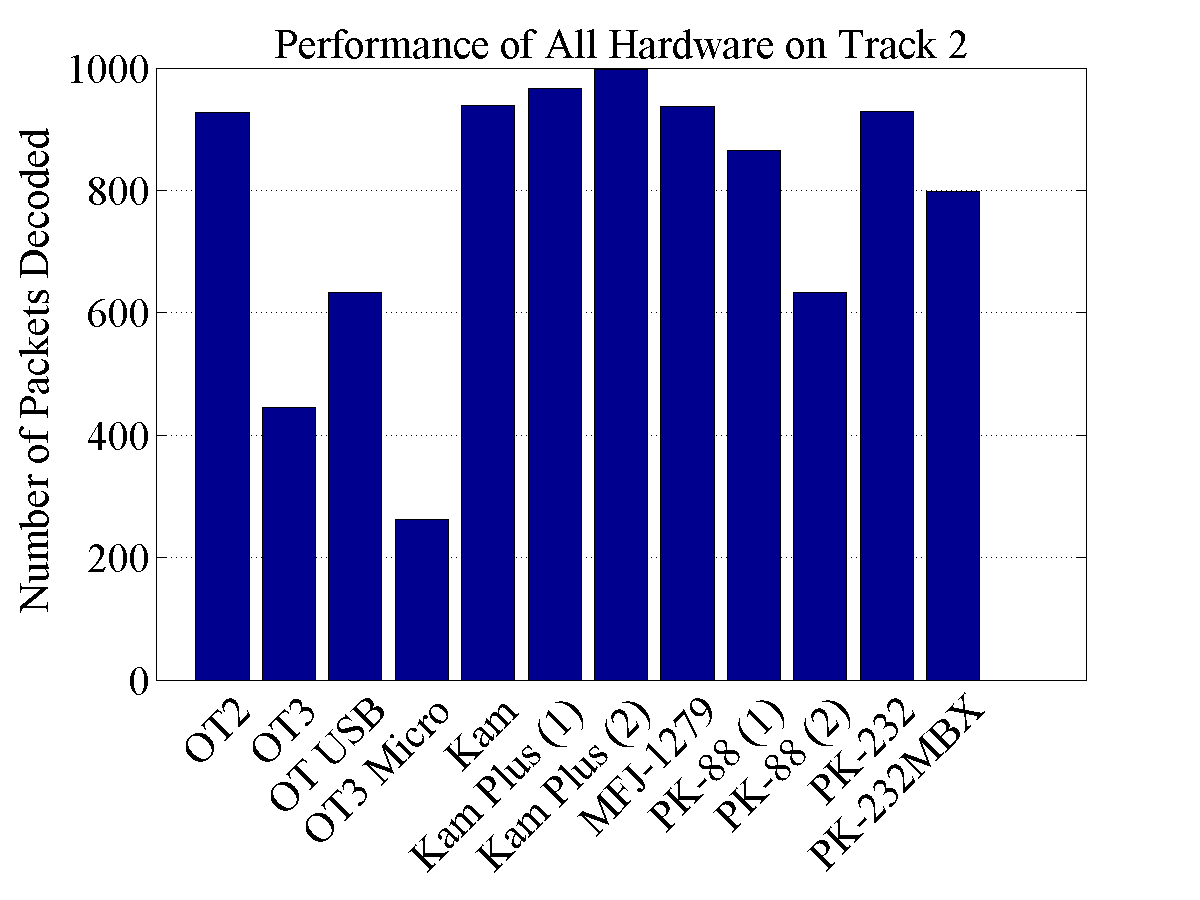
\includegraphics[width=0.75\linewidth]{images/PerformanceofAllHardwareonTrack2.png} 
	\caption{Number of packets successfully decoded for all tested hardware on the Track 2 test file.}
   \label{allHardwareTrack2}
\end{figure}

Using these results the best numbers for the hardware were 40 packets decoded from the Open Track 3 test, 200 from the javAX25 generated file, 25 from the Open Tracer 3 test with added noise, 1007 from Track 1 of the LA test suite, and 998 from Track 2. These best results can be used as a comparison for the software.

\section{Software Results}
In this section the number of packets that each of the demodulators in the javAX25 package was able to decode will be presented, highlighting those that were newly implemented in the course of this research. This will include the correlation approach that was already implemented before the start of this research as well as all of the new algorithms that were outlined in the previous chapter on Implementation. However, before getting the results from javAX25 there is one more data set to be introduced which is the results from another software based demodulation from AGW Packet Engine. Using this software 40 packets were decoded from the OpenTracker 3 test, 200 from the javAX25 generated file, 21 from the OpenTracker 3 test with added noise, 967 from Track 1 of the LA test suite, and 497 from Track 2. The results from javAX25 end up being on par with these results as well as those of the hardware.

With a total of 13 algorithms implemented, some did well and others not at all, so as in the section on hardware results, all of the data will be presented followed by a focus on those that performed the best. In the new javAX25 software implementation the filtering was moved from its original location of being on a per demodulator level basis to a central location that allowed each of the algorithms to utilize it. Some of the algorithms ended up relying on it after tuning and others could remain independent. As such, in order to present all of the data each algorithm will not only have a result for each of the 5 test files, but also for each of the three filters used on the data. The three filters used are no filter, a 900-2500Hz bandpass filter, and the same bandpass with a 6dB attenuation of 1200Hz tones to combat the signals that were not emphasized when transmitted but were deemphasized when received. For instance, for the Zero Crossing demodulator there will be three values for the OpenTracker 3 Test file, one at each filtering, and so on for the remaining 4 test files.

In terms of the data, correlation data will be on the far left of all the plots which was the current algorithm that it was the goal to beat. The performance of no filter on the OpenTracker 3 Test can be seen in Figure \ref{OT3FiltNo}, Figure \ref{OT3Filt0} shows data with the bandpass filter, and the emphasizing filter results in Figure \ref{OT3Filt6}. It can be observed that zero crossing did not favor the filters, others were resilient, and preclocking thrived. The Generated 200 Test file is the only file that the peak demodulator performed comperably to the other techniques on. The unfiltered data from this test is in Figure \ref{Gen200FiltNo}, the bandpass data in Figure \ref{Gen200Filt0}, and the results of emphasizing the signal in Figure \ref{Gen200Filt6}. Although the generated 200 packet file and the OpenTracker test file had similar results, the results for the generated 200 were better. This can be attributed to the fact that this file has only ever existed in the digital realm, it was made and consumed there, as opposed to existing in the physical world and then recording it.

\begin{figure}
  \centering
	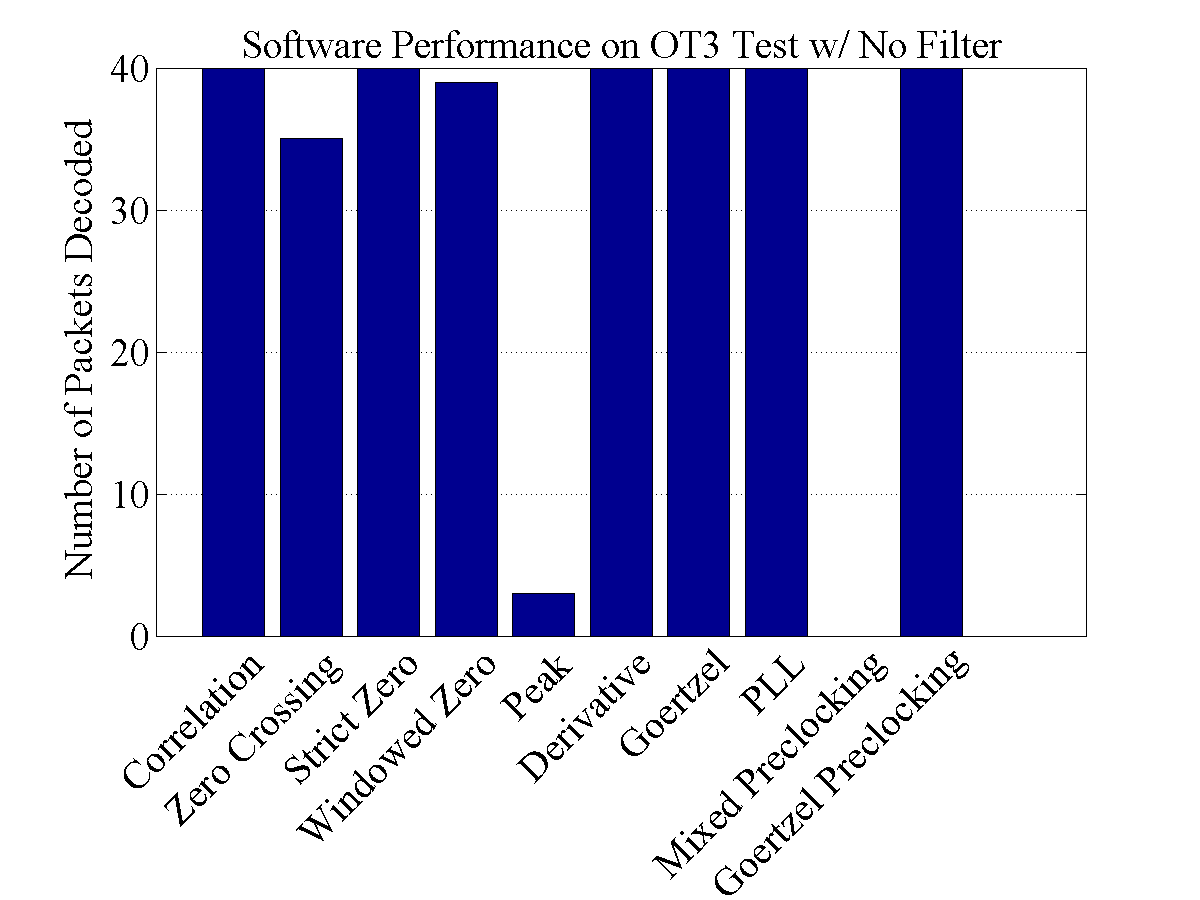
\includegraphics[width=0.75\linewidth]{images/SoftwarePerformanceonOT3TestwNoFilter.png} 
	\caption{Performance of software on the raw signal from OpenTracker 3 Test.}
   \label{OT3FiltNo}
\end{figure}
\begin{figure}
  \centering
	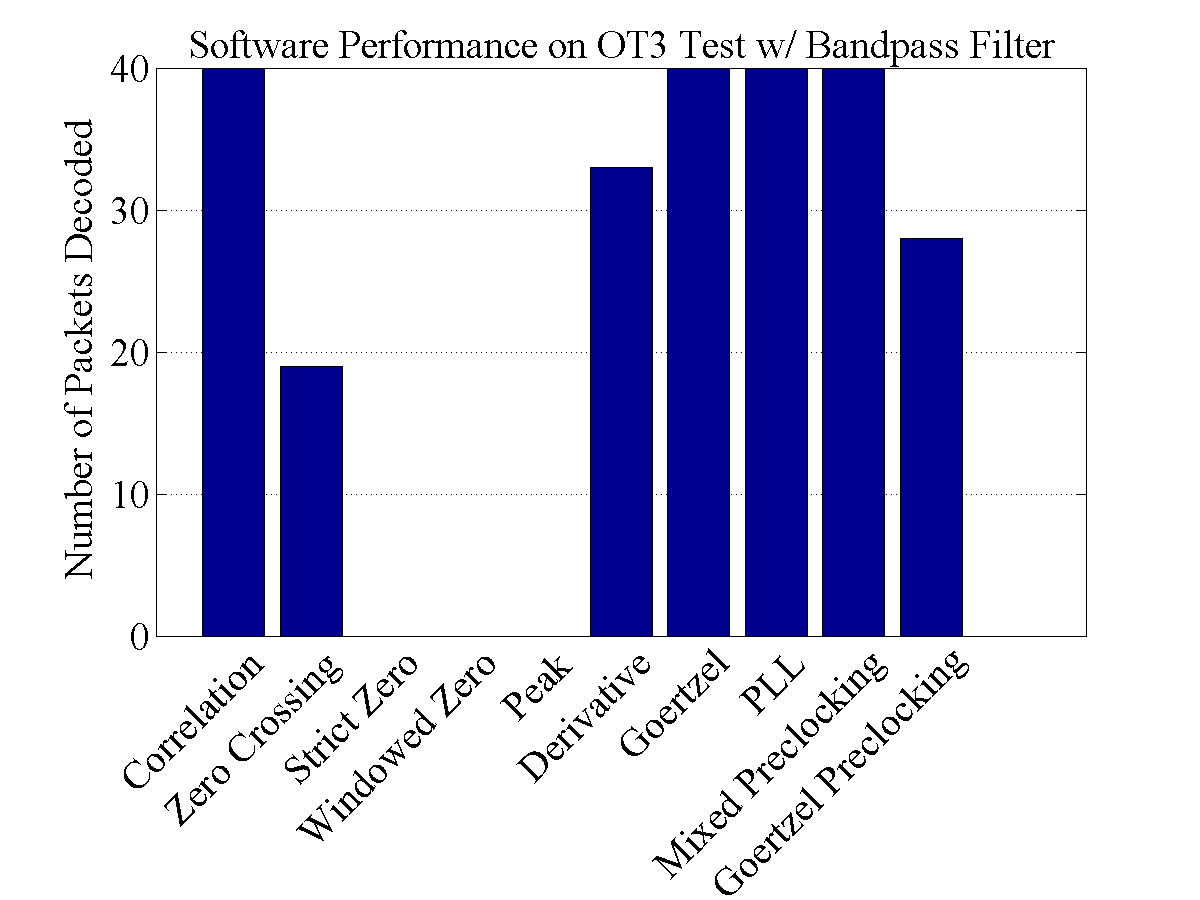
\includegraphics[width=0.75\linewidth]{images/SoftwarePerformanceonOT3TestwBandpassFilter.png} 
	\caption{Performance of software on OpenTracker 3 Test with a bandpass filter.}
   \label{OT3Filt0}
\end{figure}
\begin{figure}
  \centering
	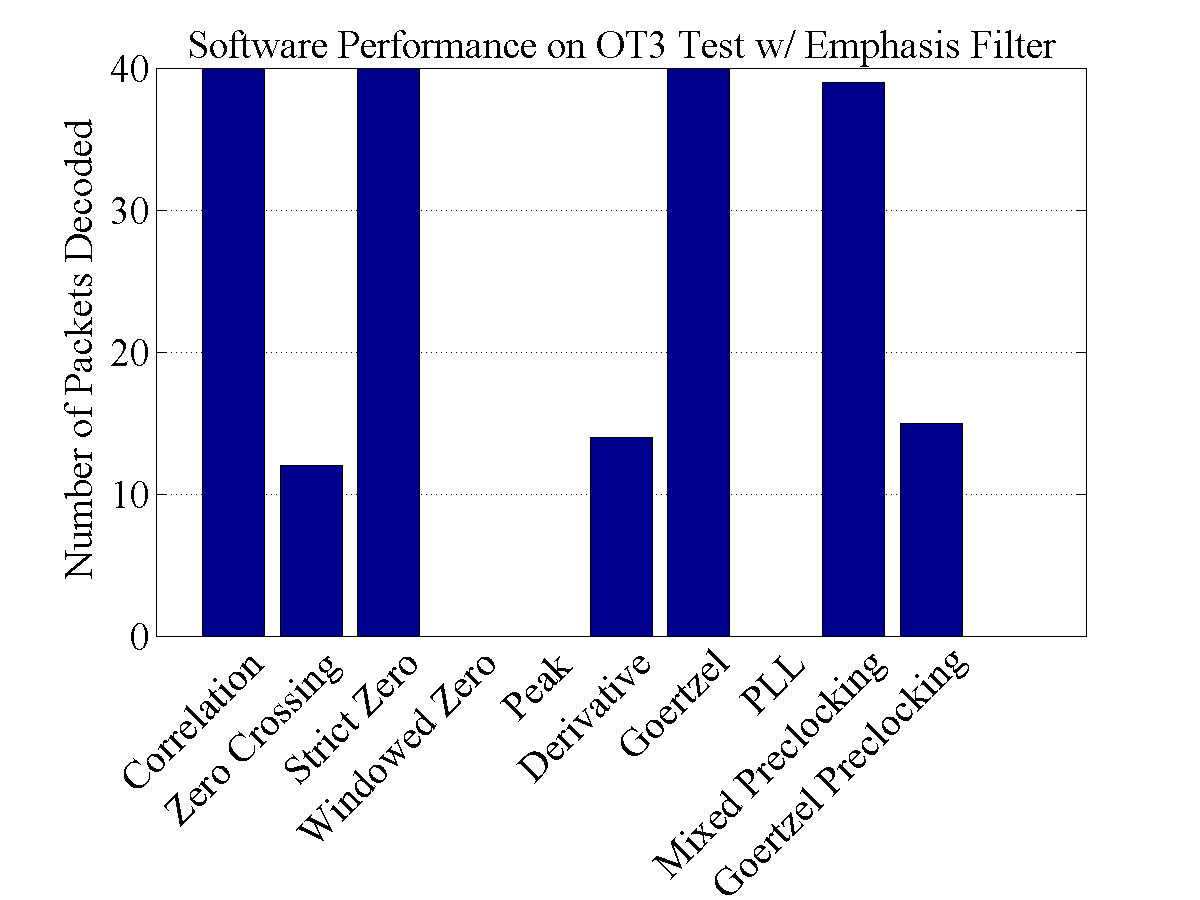
\includegraphics[width=0.75\linewidth]{images/SoftwarePerformanceonOT3TestwEmphasisFilter.png} 
	\caption{Performance of software on OpenTracker 3 Test with an emphasis filter.}
   \label{OT3Filt6}
\end{figure}
\begin{figure}
  \centering
	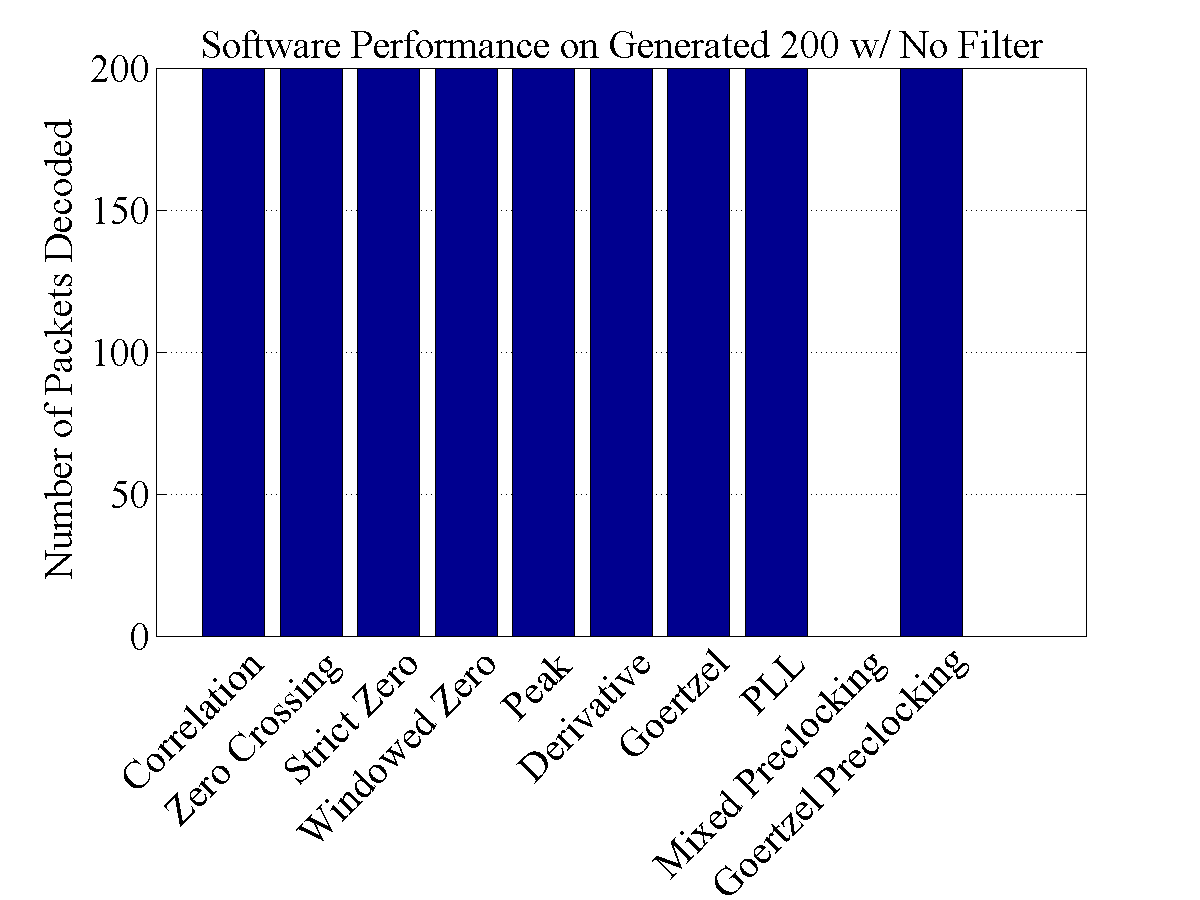
\includegraphics[width=0.75\linewidth]{images/SoftwarePerformanceonGenerated200wNoFilter.png} 
	\caption{Performance of Software on the raw signal from Generated 200.}
   \label{Gen200FiltNo}
\end{figure}
\begin{figure}
  \centering
	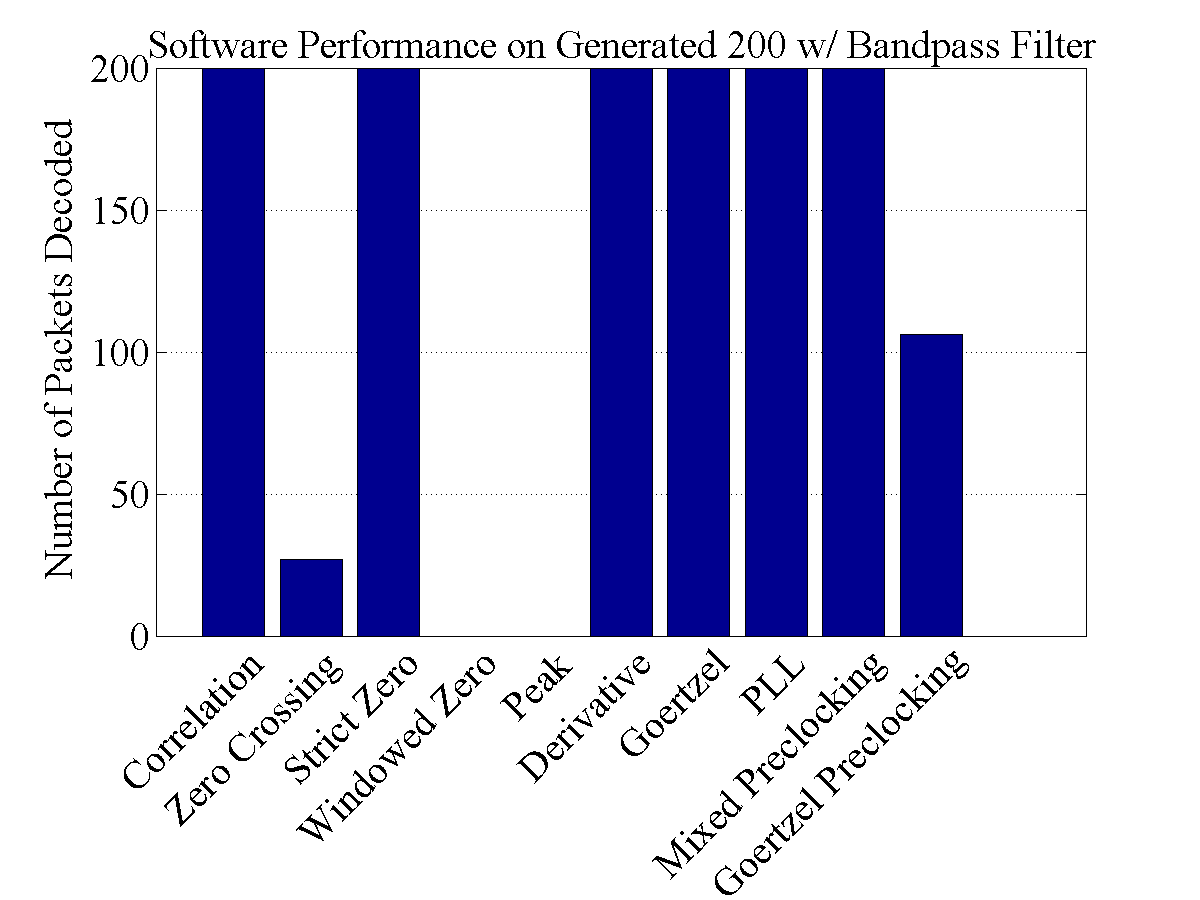
\includegraphics[width=0.75\linewidth]{images/SoftwarePerformanceonGenerated200wBandpassFilter.png} 
	\caption{Performance of software on Generated 200 with a bandpass filter.}
   \label{Gen200Filt0}
\end{figure}
\begin{figure}
  \centering
	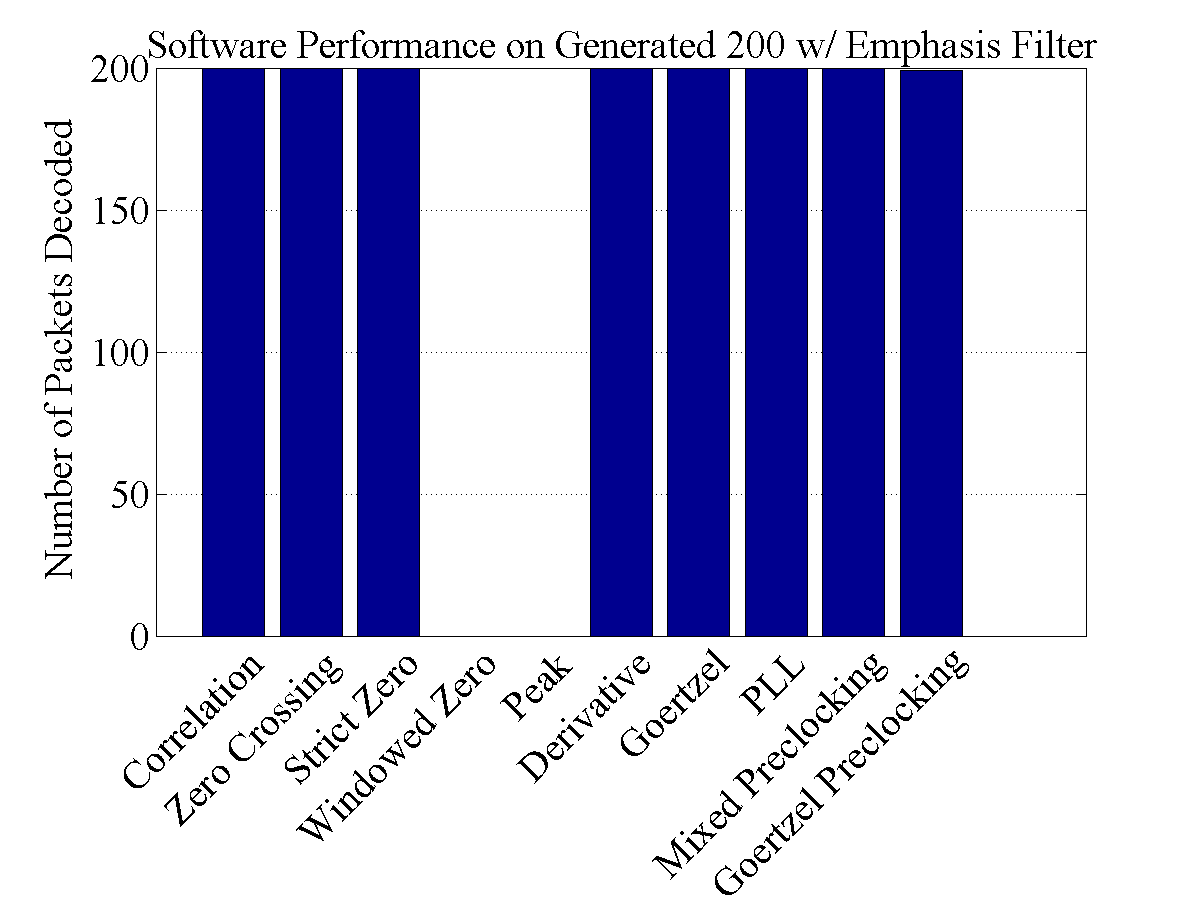
\includegraphics[width=0.75\linewidth]{images/SoftwarePerformanceonGenerated200wEmphasisFilter.png} 
	\caption{Performance of Software on Generated 200 with an emphasis filter.}
   \label{Gen200Filt6}
\end{figure}

Again, moving on from the "easy" files the performance of the software demodulators on the OpenTracker 3 Test with the noise added can be seen. Figure \ref{OTNoiseFiltNo} shows the data for the unfiltered file, Figure \ref{OTNoiseFilt0} shows bandpass filter data, and Figure \ref{OTNoiseFilt6} shows data from the emphasis filter. Two algorithms really start to shine as being comparable, and in some cases better, than the correlation demodulator. Those are the Goertzel Filter Demodulator and the PLL Demodulator. Although this is not data that was actually transmitted or received, these two start so who promise. Even the Strict Zero crossing can be seen doing well once the audio file is emphasized, but it doesn't stand up to the competition in the next two test files.

\begin{figure}
  \centering
	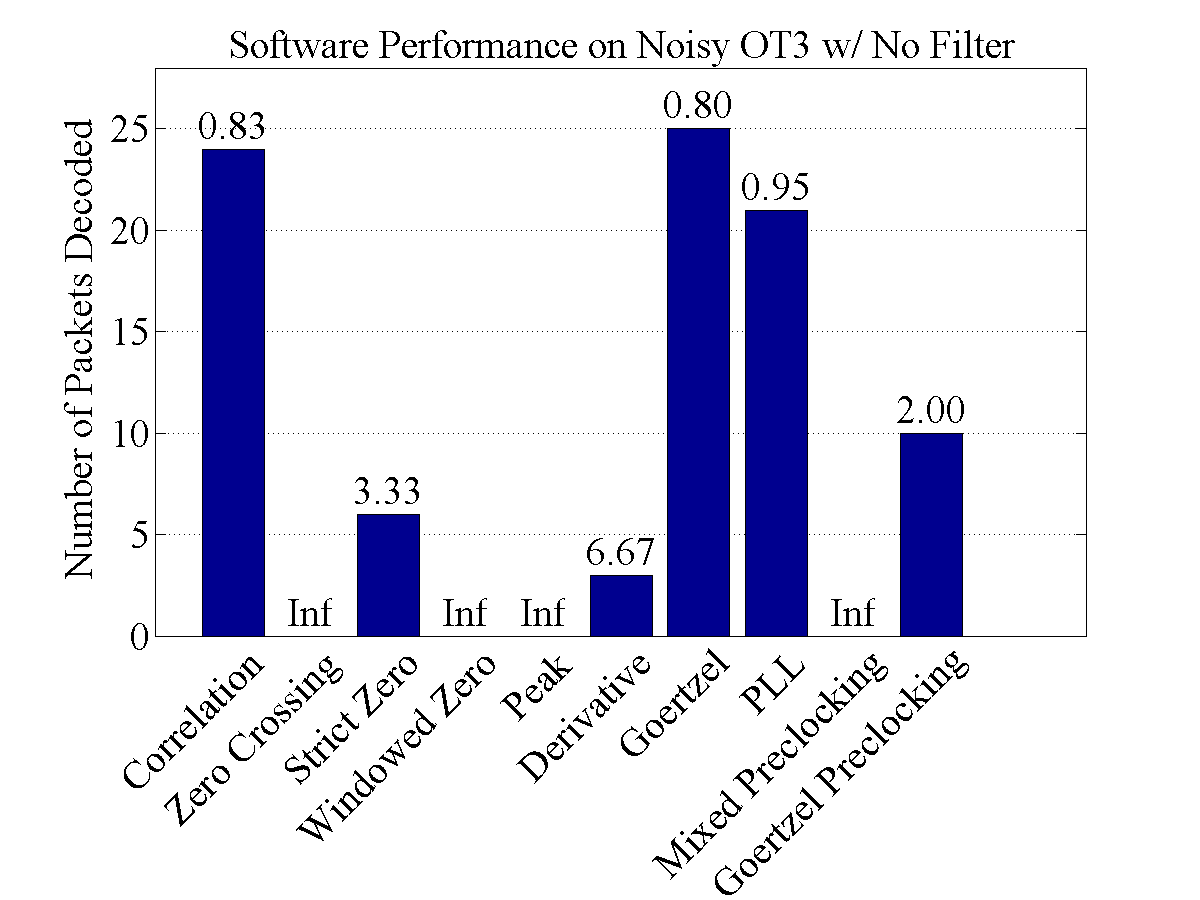
\includegraphics[width=0.75\linewidth]{images/SoftwarePerformanceonNoisyOT3wNoFilter.png} 
	\caption{Performance of software on the raw signal from OpenTracker Test with noise added.}
   \label{OTNoiseFiltNo}
\end{figure}
\begin{figure}
  \centering
	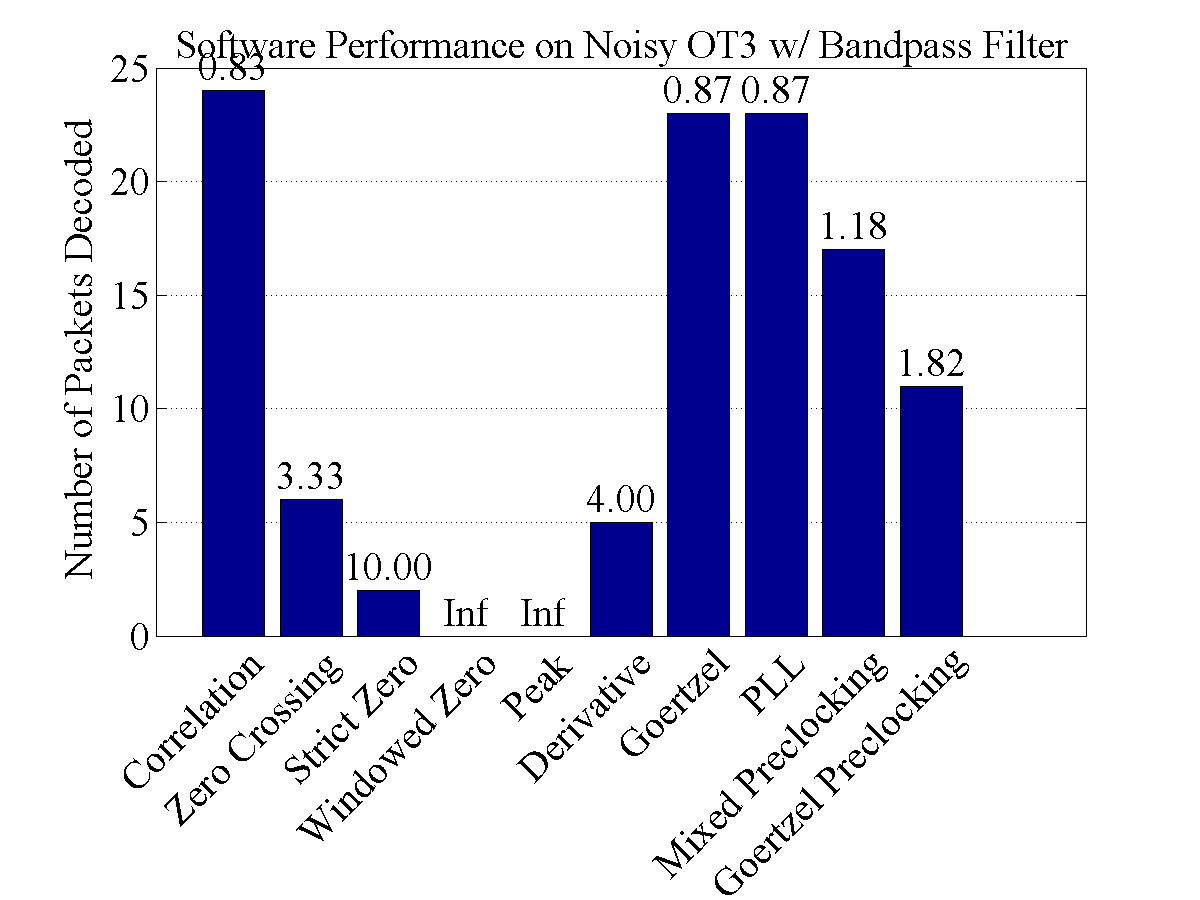
\includegraphics[width=0.75\linewidth]{images/SoftwarePerformanceonNoisyOT3wBandpassFilter.png} 
	\caption{Performance of software on OpenTracker Test with noise added with a bandpass filter.}
   \label{OTNoiseFilt0}
\end{figure}
\begin{figure}
  \centering
	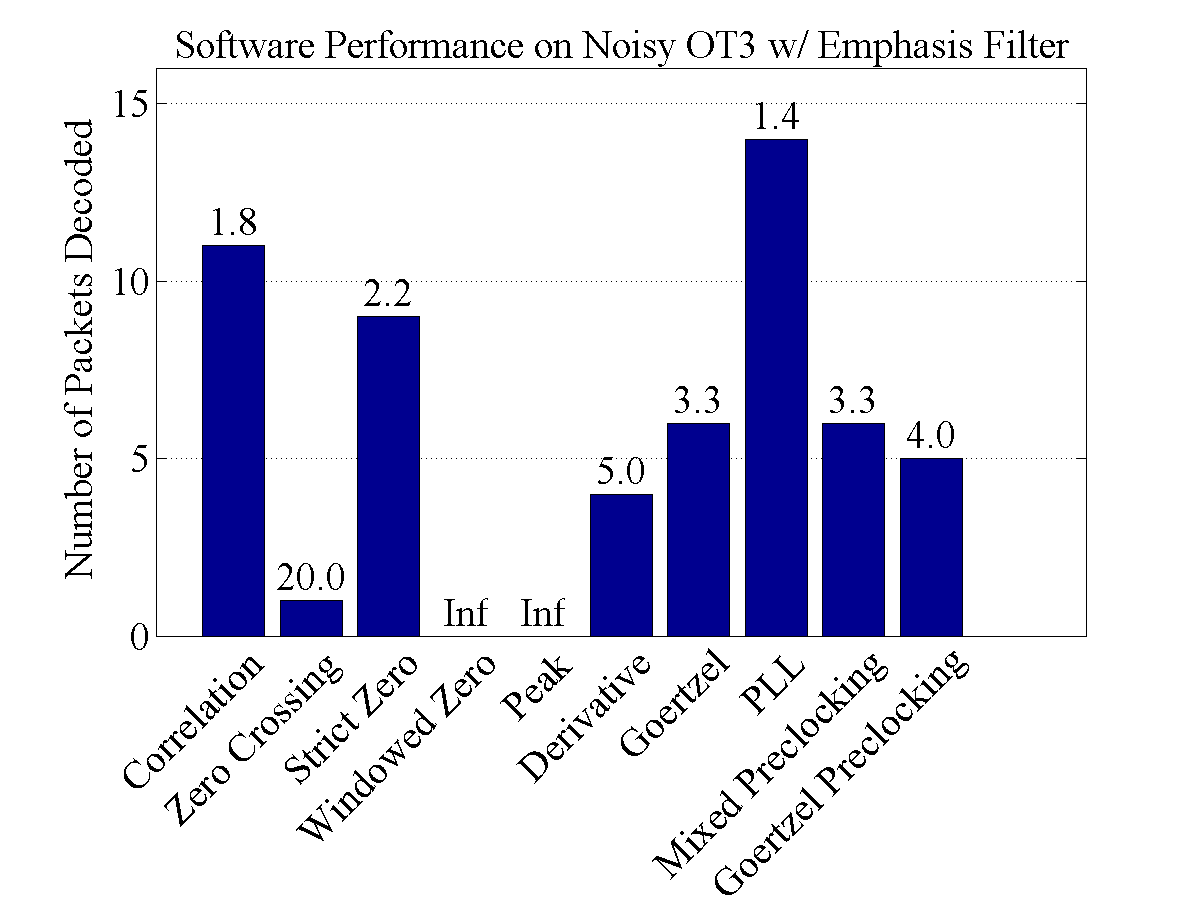
\includegraphics[width=0.75\linewidth]{images/SoftwarePerformanceonNoisyOT3wEmphasisFilter.png} 
	\caption{Performance of Software on OpenTracker Test with noise added with an emphasis filter.}
   \label{OTNoiseFilt6}
\end{figure}

As mentioned earlier, these next two test files were those that were thought the be most important to succeed at. As such, Track 1 was used to tune the algorithms since this would represent the closest real-world simulation possible. The Track 2 results are also presented for comparison. However in Track 2, in addition to being deemphasized the process of this filtering also reduced the magnitude of the signal in the audio file. As such, this file shows two things: One, the ability to pick up lower level signal and second, the algorithms tolerance to signals that were not emphasized when transmitted, but were deemphasized when received. The results of no filtering, bandpass filtering, and emphasis filtering can be seen in their respective Figure \ref{T1FiltNo}, \ref{T1Filt0}, and \ref{T1Filt6} for Track 1. The data from demodulating Track 2 can be seen in Figure \ref{T2FiltNo}, \ref{T2Filt0}, and \ref{T2Filt6}. As was caught during the OpenTracker 3 Test with noise it can be noticed that the Goertzel and PLL algorithms are still doing well on Track 1, and also the Mixed preclocking is doing fairly well. With the filter that is applied on Track 1 to create Track 2 it is basically the opposite effect of Toledo's emphasis filter and hence they cancel each other out. This can be seen by looking at the performance of the Goertzel Demodulator which does poorly with both other filterings on Track 2. However, its ability to detect low level signals and this reversal of the emphasis filtering applied makes it end of having comperable results to the just band pass filter on Track 1 - 956 versus 965. 

\begin{figure}
  \centering
	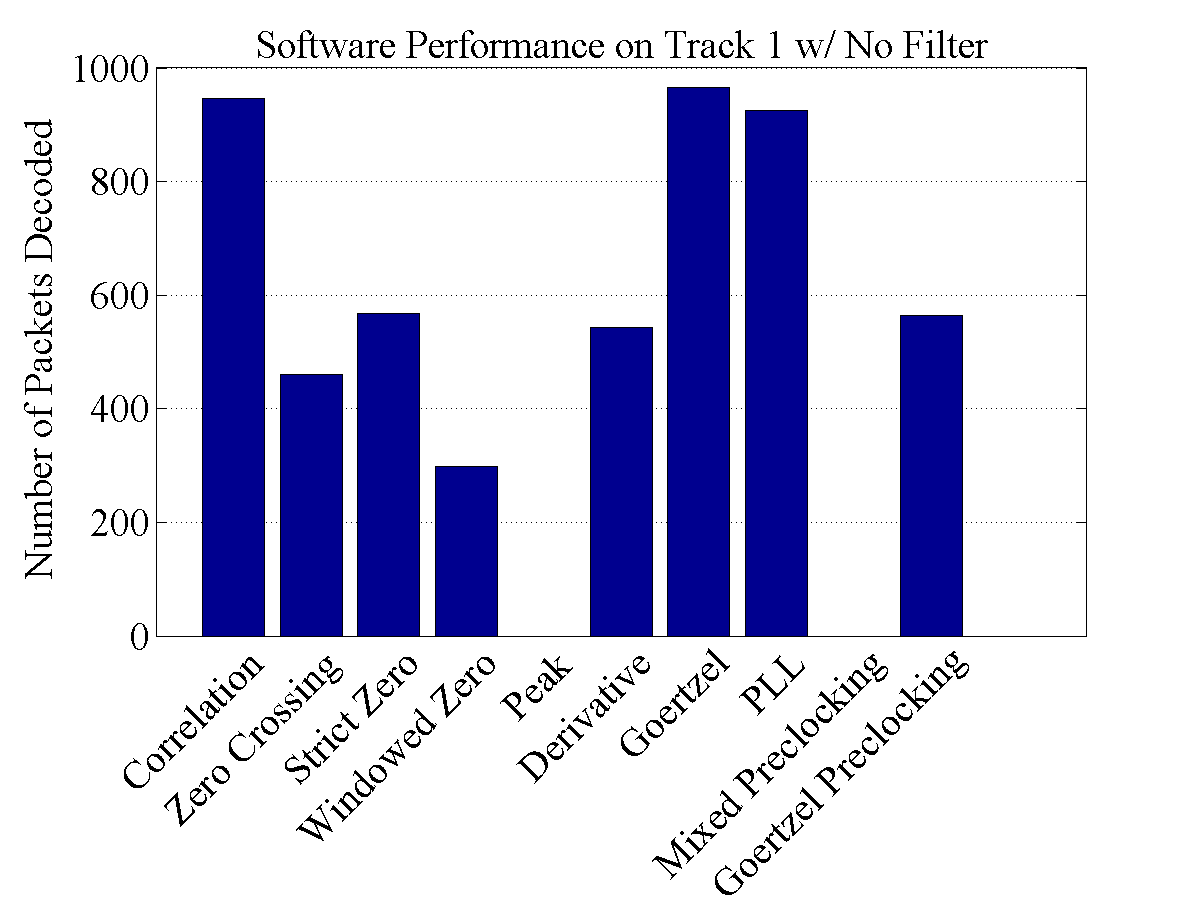
\includegraphics[width=0.75\linewidth]{images/SoftwarePerformanceonTrack1wNoFilter.png} 
	\caption{Performance of software on the raw signal from Track 1.}
   \label{T1FiltNo}
\end{figure}
\begin{figure}
  \centering
	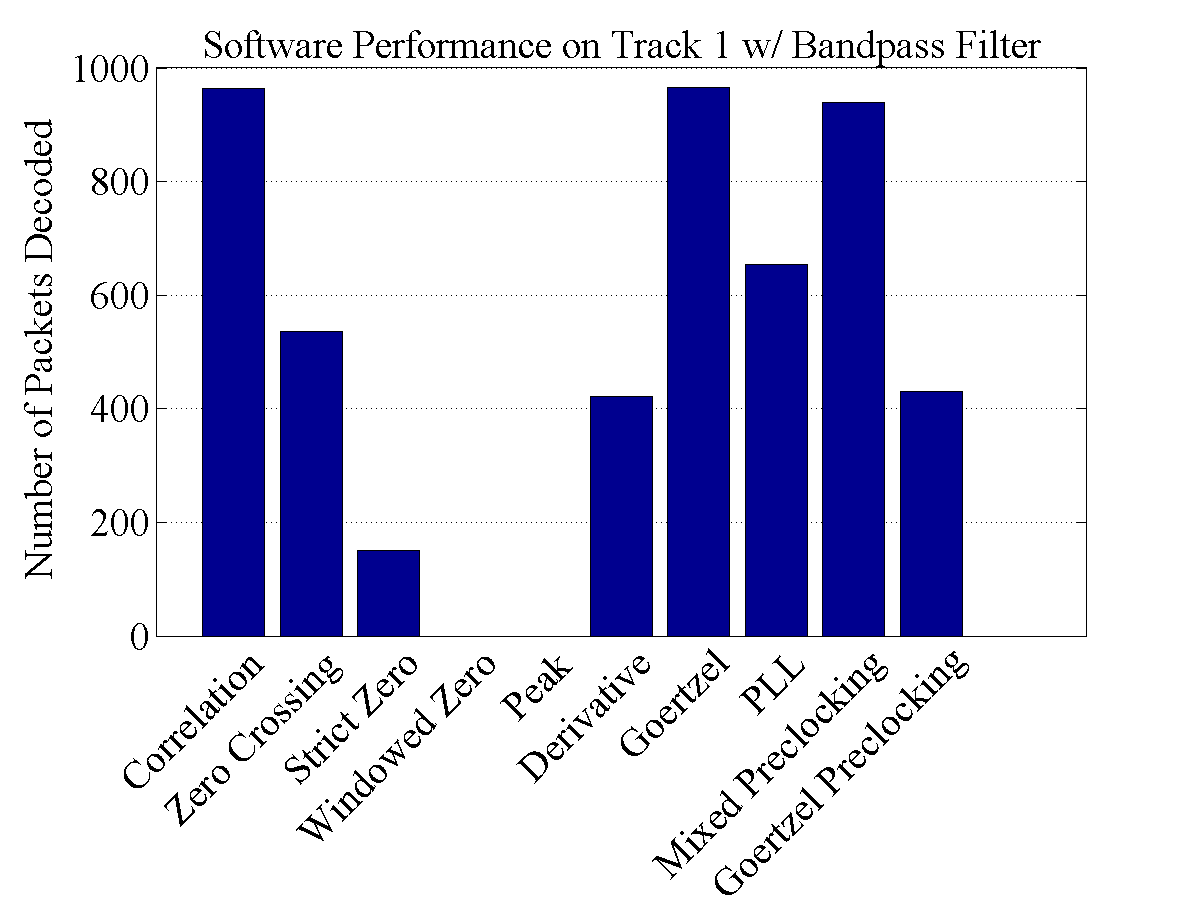
\includegraphics[width=0.75\linewidth]{images/SoftwarePerformanceonTrack1wBandpassFilter.png} 
	\caption{Performance of software on Track 1 with a bandpass filter.}
   \label{T1Filt0}
\end{figure}
\begin{figure}
  \centering
	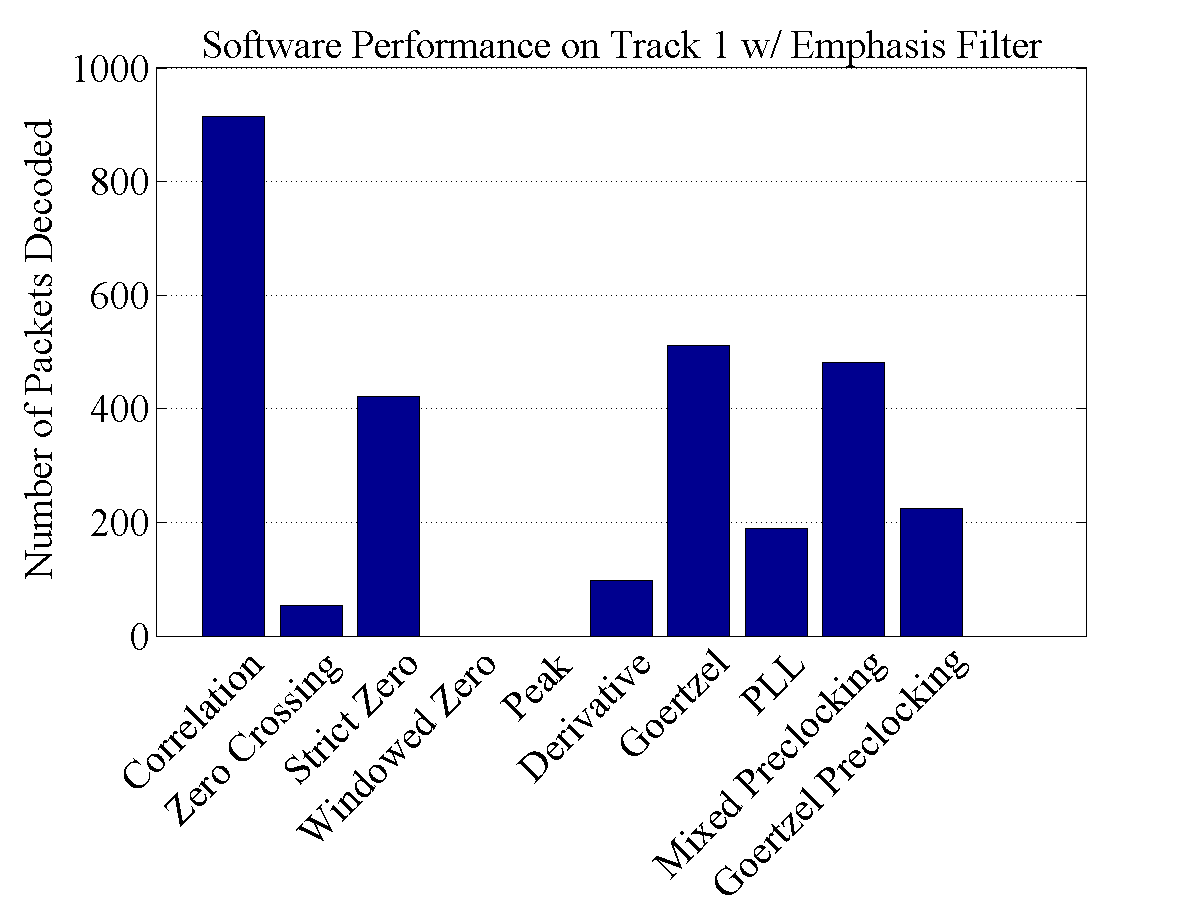
\includegraphics[width=0.75\linewidth]{images/SoftwarePerformanceonTrack1wEmphasisFilter.png} 
	\caption{Performance of software on Track 1 with an emphasis filter.}
   \label{T1Filt6}
\end{figure}
\begin{figure}
  \centering
	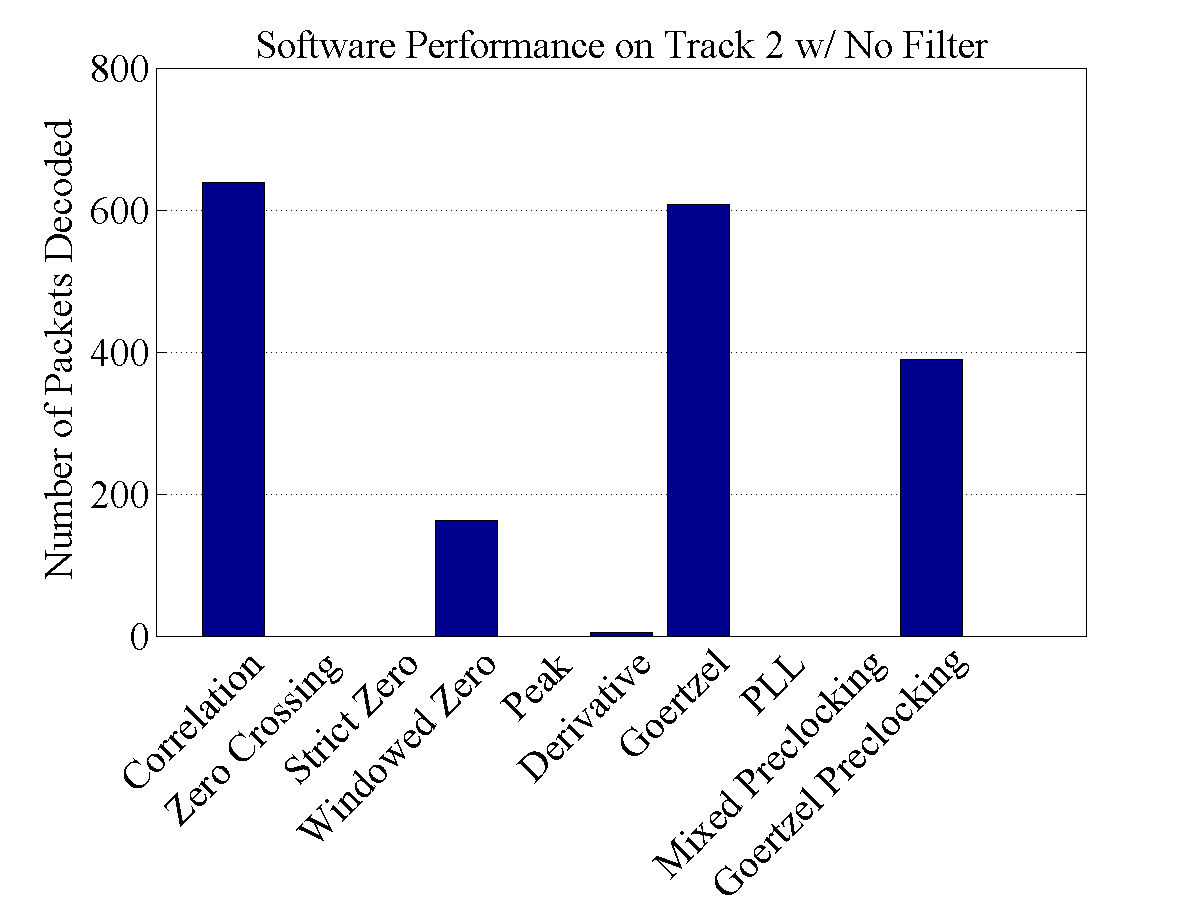
\includegraphics[width=0.75\linewidth]{images/SoftwarePerformanceonTrack2wNoFilter.png} 
	\caption{Performance of software on the raw signal from Track 2.}
   \label{T2FiltNo}
\end{figure}
\begin{figure}
  \centering
	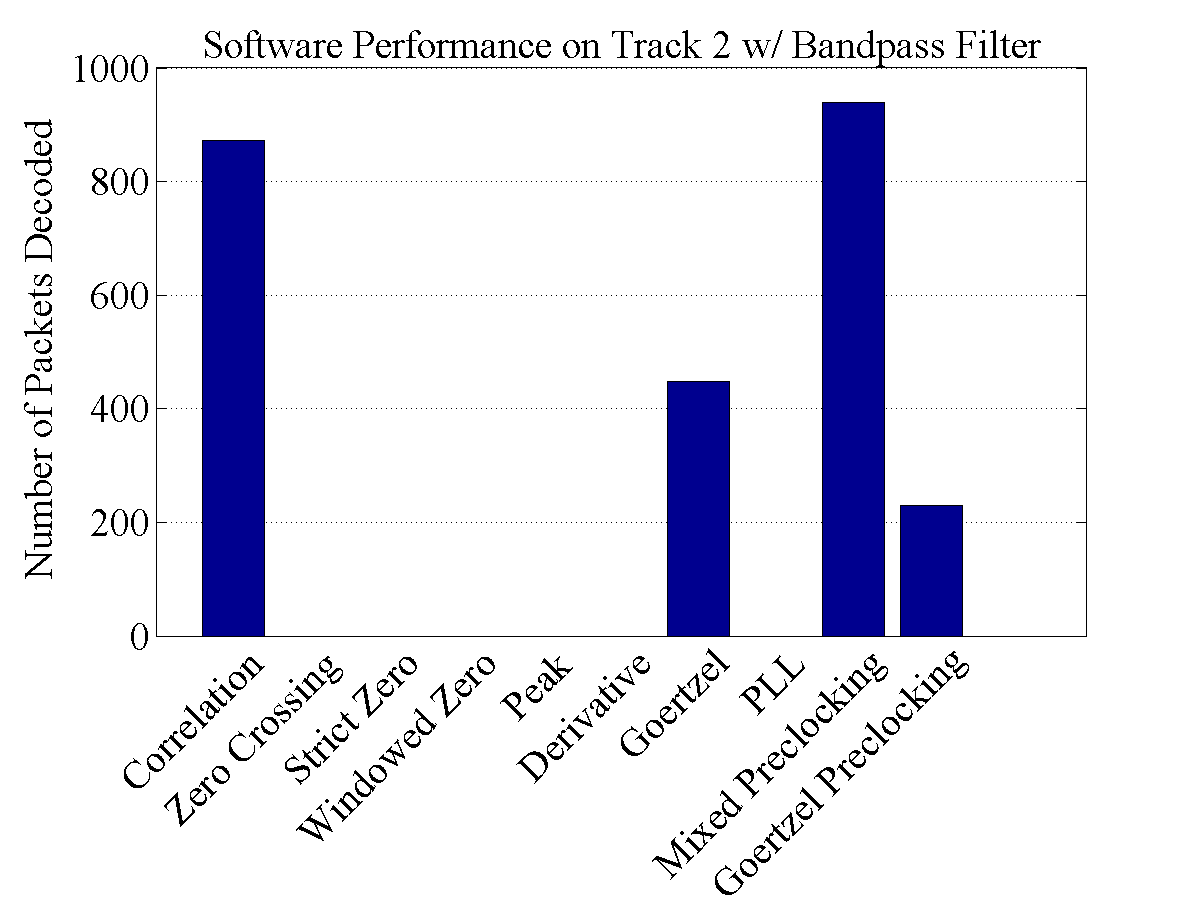
\includegraphics[width=0.75\linewidth]{images/SoftwarePerformanceonTrack2wBandpassFilter.png} 
	\caption{Performance of software on Track 2 with a bandpass filter.}
   \label{T2Filt0}
\end{figure}
\begin{figure}
  \centering
	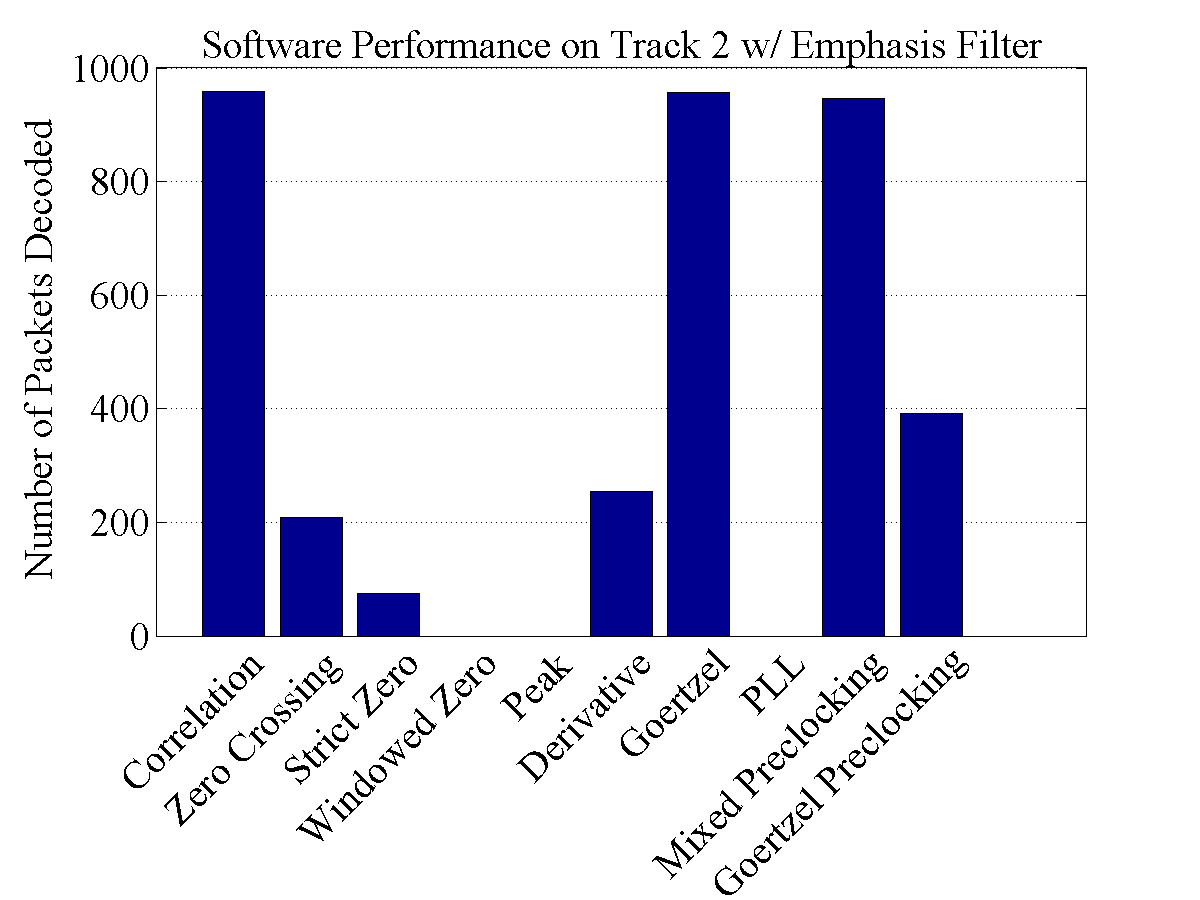
\includegraphics[width=0.75\linewidth]{images/SoftwarePerformanceonTrack2wEmphasisFilter.png} 
	\caption{Performance of software on Track 2 with an emphasis filter.}
   \label{T2Filt6}
\end{figure}


\subsection{Hardware and Software Comparisons}
It is now time to actually compare the new software implementations to the old ones as well as to the hardware. The first thing to notice is that the Goertzel Filter did very well, and in some cases better than the original correlation. Secondly, the complicated preclocking algorithm was also able to hold its own and still be a top contender. In fact the top three software algorithms were Correlation, Goertzel, and Mixed Preclocking with 964, 965, and 939 packets decoded from Track 1 with the bandpass filter. Even though they all have different number of packets decoded they each still have their expertise with being able to exclusively decode packets that others could not. For instance when the three are run together there is a total of 975 packets decoded due to the fact that Goertzel gets 12 packets that the other two do not, Correlation gets 7 that the others do not, and Preclocking decoded 3 that these other two missed. This could still be a good argument for the use of hardware over software since it is very easy to run multiple demodulators in parallel. Especially since the cost of this is only 5 minutes and 2 seconds on a file that is 25:49 long.

The question is, is the software better than the hardware? Looking at the highest numbers, no, but looking at the bigger picture, maybe. One thing about the hardware is that it is prone to variations and in need of periodic tuning. So, if instead of looking at the best of the breed, the average values are compared under the presumption that this would correspond to the average ham's decoding capabilities, then the software does decode more packets. Additionally, the software does not have any capacitors that will dry up or solder joints that may become brittle and affect the performance. The performance of the software today will be exactly the same in 5, 10, many years. The average number of packets decoded by the hardware on Track 1 was 935. Looking at this value any one of the three algorithms that are the top performers would be considered better.

%\chapter{Future Work}
The sections in this chapter will explain some aspects that this project uncovered that have the potential for future research. There are three main items that I think should be explored in more depth as future work in this area of AX.25 software based demodulation, they are the discrete Short-Time Fourier Transform, the use of the checksum for forward error correction, and to actually integrate these demodulators with live traffic from a radio.

\section{The Discrete Short-Time Fourier Transform}
In a paper by Zhonghui-Chen et. al. methods are outlined to use the discrete short-time Fourier transform (DSTFT) to demodulate a binary frequency shift keyed (BFSK) signal. After a discussion of the DSTFT they go into their specific implementation, but this appears to show promise because of there results section. Granted this was for a simulation buy they showed that the error rate was lower using the DFTFT than traditional coherent demodulation even for lower signal to noise ratios \cite{Chen2008}

\section{Use the CRC for FEC}
Each AX.25 packet contains a checksum that is generated by using a cyclic redundancy check (CRC). This is used by all demodulators in order to determine if the packet that the demodulator thinks it decoded was actually a legitimate packet or just noise that happened to look like a packet. Although the CRC was not intended for forward error correction (FEC), it would be interesting to see the effects of using it as such. With algorithms such as the Goertzel algorithm the power of each symbol is determined and this power could be used to assign a level of confidence on that demodulated bit. If a packet fails the CRC check, but all except for one of the bits has a confidence greater than 80 percent, would the CRC pass if that one bit was flipped to the other symbol? This is a very good argument for the use of software since this meta data about the decoding of the packets can be kept in memory, something that most hardware is very light on. 

\section{Integrations with a Radio}
Finally another area for future work would be to integrate the new algorithms with a radio and use them to decode live data. Although the data used in the testing was a recording of live data, it would be very gratifying to be able to see these algorithms decode audio straight from the radio. Inside of javaAX25 the packages should already support it, so it should be a matter of just setting it up and letting it run. This analysis would allow for verification of the implementations functionalities as well as to be able to see how the different algorithms perform side by side in real time.


%\chapter{Conclusion}
This research set out to try and prove that software could do AX.25 demodulation better than the hardware. Depending on perspective, it may have done so. However, at the very least the research shows that there are many ways to approach the challenge of demodulating these packets and presents the relative performance of over 10 software based approaches and 12 dedicated hardware approaches, whether that hardware is an OpenTracker or TNC.

In the end, the software did do better than the average result using hardware, but in the primary benchmarking file, software was only able to decode 975 packets as opposed to the 1007 that the best piece of hardware detected. Exploring some of the items in the future work section such as using the checksum for forward error correction may be able to get software to the same level as hardware, as it is close.

\end{document}
